% !TeX spellcheck = en_US
% !TeX encoding = UTF-8
% !TEX program = pdflatex

% VSCODE word wrap: ALT + Z
% COMPILE WITH:
% `latexmk`
% latexmk -pdf main.tex
% You need pdflatex and biber (in all TeXLive distributions)

\documentclass[11pt]{book} % text width
\usepackage[utf8]{inputenc} % encode text to utf8

% paragraph formatting: https://www.overleaf.com/learn/latex/Paragraph_formatting
\setlength{\parindent}{1em}
\setlength{\parskip}{1em}

% better language support
\usepackage[english]{babel}

% use pdflatex
\usepackage[T1]{fontenc} % font encoding
\usepackage[a4paper, margin=2cm, head=18.0pt]{geometry} % set margins to 1.5 cm
\usepackage{graphicx}% for graphics
\usepackage[onehalfspacing]{setspace}
\usepackage{tocbasic}
\usepackage{booktabs}
\usepackage{multicol}
\usepackage{multirow}
\usepackage[]{scrlayer-scrpage}
\usepackage[titletoc]{appendix}
\usepackage{comment}

\usepackage{dirtree} % directory tree
\usepackage{float} % float images
\usepackage{microtype} % better text formatting, avoid one word on a new line for example
\usepackage{mathtools} % math tools
\usepackage{amssymb} % math symbols
\usepackage{algorithm} % algorithm
% \usepackage{algorithmic}  % old, use algorithmicx from algpseudocode
\usepackage{algpseudocode} % pseudocode

% fix Font shape `T1/fve/m/sc' undefined on \Procedure
\renewcommand{\algorithmicprocedure}{\textbf{Procedure}}

\usepackage{tikz} % for drawing graphs
%\usetikzlibrary{positioning} % for relative positioning of nodes

% quotes and bibliography: https://www.overleaf.com/learn/latex/Typesetting_quotations
\usepackage{csquotes}
\usepackage[
    % Use the french style of quotes, which are more visibly distinct
    left = \flqq{},% 
    right = \frqq{},% 
    leftsub = \flq{},% 
    rightsub = \frq{} %
]{dirtytalk}
\DeclareQuoteStyle{english}{\glqq}{\grqq}{\glq}{\grq}

% \usepackage[
%     backend=biber,
%     style=numeric,
%     sorting=none
% ]{biblatex}
%\usepackage[backend=biber, style=numeric, defernumbers=true, language=american]{biblatex}
\usepackage[backend=biber, style=numeric, sorting=none, defernumbers=true, language=american]{biblatex}
% add commands for automatic cite/uncite distinction
\DeclareBibliographyCategory{cited}
\AtEveryCitekey{\addtocategory{cited}{\thefield{entrykey}}}
\addbibresource{biblio.bib} % bibliography
\nocite{*} % all references

\newcommand{\ts}{\textsuperscript} % superscript for 2nd or XIXème

\pagenumbering{roman} % set page numbering of front matter sections

% use acronyms and glossaries
% toc: add glossary to table of contents
\usepackage{hyperref}
\usepackage{xurl}
\usepackage[acronym, toc]{glossaries} 
\makeglossaries
\newglossaryentry{memgraph}
{
  name=memory graph,
  description={A memory graph, or \textit{memgraph} is a graph representation of a memory dump. This graph can be a graph of blocks, where each node in the graph corresponds to a block of 8 bytes in the heap dump and each edge corresponds to a pointer from one block to another, or describes which blocks are part of a chunk whose root note is a Chunk Header Node. It can also be a graph of objects, where each node in the graph corresponds to a chunk in heap dump and each edge corresponds to a pointer from one object to another.}
}

\newglossaryentry{nodes}
{
  name=nodes,
  description={A node is an entity in a graph, it can be a person, a place, a thing, or any other entity.}
}
\newglossaryentry{chn}{
  name={CHN},
  description={Chunk Header Node. This is a node whose bytes have been identified as a data structure header. In the graph, this node is the root node of an malloc-allocated memory chunk.}
}

\newglossaryentry{pn}{
  name={PN},
  description={Pointer Node. This is a node whose bytes have been identified as a pointer.}
}

\newglossaryentry{kn}{
  name={KN},
  description={Key Node. This is a node whose bytes have been identified as a key. This identification relies both on the annotations and some verification checks.}
}

\newglossaryentry{vn}{
  name={VN},
  description={Value Node. These are all blocks that have not been identified. It is the default node type.}
}

\newacronym{kg}{KG}{Knowledge Graph}
\newacronym{foss}{FOSS}{Free and Open Source Software}
\newacronym{rdf}{RDF}{Resource Description Framework}
\newacronym{rdfs}{RDFS}{Resource Description Framework Schema}
\newacronym{owl}{OWL}{Web Ontology Language}
\newacronym{ml}{ML}{Machine Learning}
\newacronym{dl}{DL}{Deep Learning}
\newacronym{fe}{FE}{Feature Evaluation}
\newacronym{nlp}{NLP}{Natural Language Processing}
\newacronym{ke}{KE}{Knowledge Engineering}
\newacronym{del}{DEL}{Directed Edge-labelled Graphs}
\newacronym{er}{ER}{Entity Resolution}
\newacronym{qa}{QA}{Quality Assurance}
\newacronym{sparql}{SPARQL}{SPARQL Protocol and RDF Query Language}
\newacronym{ssh}{SSH}{Secure Shell Protocol}
\newacronym{os}{OS}{Operating System}
\newacronym{vm}{VM}{Virtual Machine}
\newacronym{ddos}{DDoS}{Distributed Denial of Service}
\newacronym{ess}{ESS}{Estimated Security Strength}
\newacronym{vmi}{VMI}{Virtual Machine Introspection}
\newacronym{smote}{SMOTE}{Synthetic Minority Over-sampling Technique}
\newacronym{svm}{SVM}{Support Vector Machine}
\newacronym{knn}{KNN}{K-Nearest Neighbors}
\newacronym{rf}{RF}{Random Forest}
\newacronym{mlp}{MLP}{Multi-Layer Perceptron}
\newacronym{relu}{ReLU}{Rectified Linear Unit}
\newacronym{sgd}{SGD}{Stochastic Gradient Descent}
\newacronym{ai}{AI}{Artificial Intelligence}
\newacronym{pca}{PCA}{Principal Component Analysis}
\newacronym{lda}{LDA}{Linear Discriminant Analysis}
\newacronym{tsne}{t-SNE}{t-distributed Stochastic Neighbor Embedding}
\newacronym{msb}{MSB}{Most Significant Bit}
\newacronym{lsb}{LSB}{Least Significant Bit}

%deep learning
\newacronym{lstm}{LSTM}{Long Short-Term Memory}
\newacronym{gru}{GRU}{Gated Recurrent Units}
\newacronym{rnn}{RNN}{Recurrent Neural Networks}
\newacronym{cnn}{CNN}{Convolutional Neural Networks}
\newacronym{rcnn}{RCNN}{Recurrent Convolutional Neural Network}
\newacronym{gnn}{GNN}{Graph Neural Network}
\newacronym{gcn}{GCN}{Graph Convolutional Networks}
\newacronym{llm}{LLM}{Large Language Model}

%\input{glossaries.tex} % acronyms definitions, failed to make in work on a separate file!!!

% custom commands
% escape char in latex: https://tex.stackexchange.com/questions/34580/escape-character-in-latex
% horizontal spacing: https://tex.stackexchange.com/questions/74353/what-commands-are-there-for-horizontal-spacing/74354
\newcommand{\p}{\texttt{+}} % small unary plus
\newcommand{\doublep}{\texttt{++}} % double small unary plus
\newcommand{\m}{\texttt{-} \space} % small unary minus
\newcommand{\doublem}{\texttt{-}\texttt{-} \space} % double small unary minus

% title and section formatting
\usepackage{titlesec}

\titleclass{\chapter}{straight} % make chapters act like sections
\titleformat{\chapter}
  {\normalfont\Huge\bfseries}{\thechapter}{1em}{}
\titlespacing*{\chapter}{0pt}{\parskip}{\parskip}

\setcounter{tocdepth}{3} % set depth of table of contents
\setcounter{secnumdepth}{3}  % Numbering depth of sections

% ------------------------------ code ------------------------------
\usepackage{listings} % code listings

% code listing style
\usepackage{bera}% optional: just to have a nice mono-spaced font
\usepackage{listings}
\usepackage{xcolor}

\definecolor{eclipseStrings}{RGB}{42,0.0,255}
\definecolor{eclipseKeywords}{RGB}{127,0,85}
\definecolor{punctuationcolor}{rgb}{0.5,0,0}
\definecolor{delimcolor}{rgb}{0,0.5,0}
\definecolor{red}{rgb}{1,0,0}
\colorlet{numb}{magenta!60!black}

\lstset{
  language=bash,
  basicstyle=\ttfamily\small,
  breaklines=true,
  frame=single,
  numbers=left,
  numberstyle=\tiny,
  showstringspaces=false,
  tabsize=4,
  captionpos=b
}

\lstdefinestyle{json}{
  basicstyle=\ttfamily\small,
  breaklines=true,
  postbreak=\mbox{\space},
  columns=fullflexible,
  showstringspaces=false,
  commentstyle=\color{gray},
  keywordstyle=\color{black},
  numberstyle=\tiny\color{gray},
  numbers=left,
  frame=single,
  captionpos=b
}

\lstdefinestyle{text}{
  basicstyle=\ttfamily\small,
  breaklines=true,
  postbreak=\mbox{\space},
  columns=fullflexible,
  showstringspaces=false,
  commentstyle=\color{gray},
  keywordstyle=\color{black},
  numberstyle=\tiny\color{gray},
  numbers=left,
  frame=single,
  captionpos=b
}

\lstdefinestyle{hexdump}{
  basicstyle=\ttfamily\small,
  breaklines=true,
  postbreak=\mbox{\space},
  columns=fullflexible,
  showstringspaces=false,
  commentstyle=\color{gray},
  keywordstyle=\color{black},
  numberstyle=\tiny\color{gray},
  numbers=left,
  frame=single,
  captionpos=b
}

\lstdefinestyle{rust}{
  basicstyle=\ttfamily\small,
  breaklines=true,
  postbreak=\mbox{\space},
  columns=fullflexible,
  showstringspaces=false,
  commentstyle=\color{gray},
  keywordstyle=\color{black},
  numberstyle=\tiny\color{gray},
  numbers=left,
  frame=single,
  captionpos=b
}

\usepackage{hyphenat} % fix "overfull hbox" with slicing words using hyphenation
\hyphenation{hy-phen-a-tion} % indicate all 3 permissible hyphenation points

% where to put all images and figures
\graphicspath{{img/}}

% customize the header and footer of the document
\usepackage{scrlayer-scrpage}
\clearpairofpagestyles
\cfoot[\pagemark]{\pagemark}

% document info
\newcommand{\thetitle}{Predicting SSH keys in Open SSH Memory dumps}
\newcommand{\theauthor}{Rascoussier, Florian Guillaume Pierre}

\title{\thetitle}
\author{\theauthor}
\date{April-Mai 2023}

% document content
\begin{document}

% !TeX spellcheck = en_US
% !TeX encoding = UTF-8
\begin{titlepage}
    \centering
    \begin{onehalfspace}
    	
        	
\includegraphics[width=7cm, height=1.5cm]{uni-logo.png}
			\hspace*{1.0cm}
			\includegraphics*[width=7cm, height=1.5cm]{Logo_INSA.png}\\
        	\vspace{1.0cm}
        	{\Large \bfseries Masterarbeit}\\

        	\vspace{2.5cm}

            \begin{doublespace}
            	{\textsf{\Huge{\thetitle}}}
            \end{doublespace}

        	\vspace{2cm}

            {\Large A report by}\\

        	\vspace{1cm}

        	{\bfseries \large{\theauthor}} \\
			\vspace{0.5cm}
			Matrikelnummer (Passau): 112485 \\
			Matrikelnummer (INSA): 4018543 \\


        	\vfill

        	{\Large
                \textit{Erstpr\"ufer} \\
				Prof. Dr. Harald Kosch \\
				\textit{Zweitpr\"ufer} \\
				Prof. Dr. Michael Granitzer\\
				\vspace{0.5cm}
				\textit{Betreuer} \\
				Christofer Fellicious\\
				Prof. Dr. Pierre-Edouard Portier\\
				Prof. Dr. Elöd Egyed-Zsigmond\\
        	}

        	\vspace{1cm}

        	\parbox{\linewidth}{\hrule\strut}

            \vfill

			{\large \today}
    \end{onehalfspace}
\end{titlepage}

\newpage

%%%%%%%%%%%%%%%%%%%%%%%%%%%%%%%%%%%%%%%%%%%%%%%%%%%%%%%%%%%%%%%%%%%%%%%%%%%%%%%%%%%%%%%%%

% -- ABSTRACT
\section*{Abstract}
As the digital landscape evolves, cybersecurity has become an indispensable focus of IT systems. Its ever-escalating challenges have amplified the importance of digital forensics, particularly in the analysis of heap dumps from main memory. In this context, the Secure Shell protocol (\acrshort{ssh}) designed for encrypted communications, serves as both a safeguard and a potential veil for malicious activities. This research project focuses on predicting SSH keys in OpenSSH memory dumps, aiming to enhance protective measures against illicit access and enable the development of advanced security frameworks or tools like honeypots. 

This Masterarbeit is situated within the broader SmartVMI project, a collaborative research initiative with the objective to advance artificial intelligence-based mechanisms for attack detection and digital forensics. Specifically, this work seeks to build upon existing research on key prediction in OpenSSH heap dumps. Utilizing machine learning algorithms, the study aims to refine feature extraction techniques and explore innovative methods for effective key detection prediction. The objective is to accurately predict the presence and location of SSH keys within memory dumps. This work builds upon, and aims to enhance, the foundations laid by SSHkex \cite{SSHkex22} and SmartKex \cite{SmartKex22}, enriching both the methodology and the results of the original research while exploring the untapped potential of newly proposed approaches.

This report encapsulates the progress of a year-long Master's thesis research project executed between October 2022 and October 2023. Conducted within the framework of the PhDTrack program between the University of Passau and INSA Lyon, the research has been supervised by Christofer Fellicious and Prof. Dr. Michael Granitzer from the University of Passau, as well as Prof. Dr. Pierre-Edouard Portier from INSA Lyon. It offers an in-depth discussion on the current state-of-the-art in key prediction for OpenSSH memory dumps, research questions, experimental setups, programs development as well as discussing potential future directions.

% -- Acknowledgements
\newpage
\section*{Acknowledgements}
A special acknowledgement goes to Christofer Fellicious, my engaged supervisor at the University of Passau, for his guidance, support and feedback during the Masterarbeit. 

I want to express my sincere gratitude to my colleague and friend, Clément Lahoche, whose human and technical skills have been a great source of inspiration and motivation throughout this project;  especially considering that we have been working on closely related subjects. It has been a great pleasure to share our ideas and insights, and to collaborate on the development of several programs necessary for the experimentation. 

Another acknowledgements go to my esteemed supervisors Prof. Dr. Granitzer and Prof. Dr. Portier for their support and feedback during the Masterarbeit. 

I would also like to express my sincere gratitude to all the persons that have helped me, even punctually, during the Masterarbeit with their valuable help, insights, discussions and contributions as well as all the persons involved in the PhDTrack program that made this Masterarbeit possible, including but not limited to: 
\begin{itemize}
    \item Lionel Brunie, Director of CS Department at INSA Lyon, that makes this PhDTrack program possible from the French side.
    \item Harald Kosch, Head of the Chair of Distributed Information Systems at the University of Passau, that makes this PhDTrack program possible from the German side.
    \item Natalia Lucari, PhDTrack coordinator at INSA Lyon, for her support and help during the PhDTrack program.
    \item Ophelie Coueffe, PhDTrack coordinator at the University of Passau, for her support and help during the PhDTrack program.
    \item Elöd Egyed-Zsigmond, PhDTrack coordinator at the University of Passau, for the subject selection and administrative support.
    \item All the other PhDTrack students for the great atmosphere, mutual help and the interesting discussions during almost two years.
\end{itemize}

I cannot forget to 

Finally, my last acknowledgements go to my family and friends for their support and encouragements.

\newpage
% table of content with list of figures & tables
\tableofcontents
%\listoffigures
%\listoftables
\newpage

%%%%%%%%%%%%%%%%%%%%%%%%%%%%%%%%%%%%%%%%%%%%%%%%%%%%%%%%%%%%%%%%%%%%%%%%%%%%%%%%%%%%%%%%%
\pagenumbering{arabic} % reset page numbering of main matter sections

\section{Introduction}\label{chap:introduction}


Motivate your research and outline the research gap in this chapter. Why is your thesis relevant and what do you address, what has not been addressed before. 

General Requirements to the thesis:

\begin{itemize}
	\item 60 pages of content in this format. Content does not include table of content, lists, appendices etc.
	\item Proper scientific referencing
	\item Introduction and Background should be less than 50\% of the thesis
	\item Images should be readable and in the proper size. 
\end{itemize}


\section{Research Questions}

Write down and explain your research questions (2-5)
The initial objective of this thesis is to answer the following research questions:
\begin{itemize}
	\item RQ1: What is the state of the art in the field of security key detection in heap dump memory?
	\item RQ2: What are the challenges in the field of security key detection in heap dump memory?
\end{itemize}

\section{Structure of the Thesis}

Explain the structure of the thesis. 

\section{Example citation \& symbol reference}\label{sec:citation}
For symbols look at \cite{latex_symbols_2017}.


\section{Example reference}
Example reference: Look at chapter~\ref{chap:introduction}, for sections, look at section~\ref{sec:citation}.

\section{Example image}

\begin{figure}
	\centering
	
\includegraphics[width=0.5\linewidth]{uni-logo}
	\caption{Meaningful caption for this image}
	\label{fig:uniLogo}
\end{figure}

Example figure reference: Look at Figure~\ref{fig:uniLogo} to see an image. It can be \texttt{jpg}, \texttt{png}, or best: \texttt{pdf} (if vector graphic).

\section{Example table}

\begin{table}
	\centering
	\begin{tabular}{lr}
		First column & Number column \\
		\hline
		Accuracy & 0.532 \\
		F1 score & 0.87
	\end{tabular}
	\caption{Meaningful caption for this table}
	\label{tab:result}
\end{table}

Table~\ref{tab:result} shows a simple table\footnote{Check \url{https://en.wikibooks.org/wiki/LaTeX/Tables} on syntax}
\section{Background}\label{chap:background}


Introduce the related state-of-the-art and background information in order to understand the method developed in the thesis. 
\chapter{Related Work}\label{chapter:related_work}

% Purpose: To situate your work within the broader academic landscape and to show how your work is different from, or builds upon, previous research.
%
% Content:
%     + Summary and critique of existing research closely related to your own work
%     + Methodologies, results, and conclusions from existing literature
%     + Gaps in the existing research that your work aims to fill
%
% Audience: Assumes the reader understands the basic concepts and is more interested in the nuances and advancements in the specific area of research.

Now that the necessary background has been established, this chapter will present the related work in the field of machine learning for memory forensics in the context of OpenSSH. The chapter is divided into two parts. The first part will present the related work in the field of memory forensics, and the second part will present the related work in the field of machine learning for memory forensics.

\section{SSHKex}\label{sec:background:kex:sshkex}
    
SSHKex is a research project that aims to address the challenges of analyzing encrypted SSH traffic by leveraging \acrfull{vmi} techniques. Developed by \citeauthor{SSHkex22}, the project focuses on extracting SSH keys and decrypting SSH network traffic in a stealthy, non-intrusive manner while maintaining evidence integrity \cite{SSHkex22}. This paper is itself a continuation of the work presented in \citetitle{SarraceniaSSHHoneypot18} \cite{SarraceniaSSHHoneypot18}, which introduced Sarracenia, a high-interaction SSH honeypot. It is also related to a range of other research projects and papers \cite[section 5.6 and 6]{SSHkex22}.

The SSHKex approach combines standard network traffic capturing methods with dynamic SSH session key extraction. It assumes that the SSH implementation running on the server is known, which is crucial for the key extraction process. The project employs VMI tools like LibVMI and Volatility to gain a complete and untainted view of all guest VM's state information. This allows to efficiently locate SSH session keys in the main memory of a Linux machine. 

Here is a summary of the SSHKex methodology for key extraction:
\begin{enumerate}
    \item \textbf{Data Structure Information:} The method leverages detailed knowledge about the data structures used to store the keys. Specific debugging symbols corresponding to the SSH implementation version on the target system provide essential offset values to facilitate the extraction of key material. The structures of interest include \texttt{struct ssh}, \texttt{struct session\_state}, \texttt{struct newkeys}, and \texttt{struct sshenc}. These structures store a range of information such as IP addresses, ports, session states, and encryption keys.

    \item \textbf{Tracing OpenSSH Functions:} Function tracing is employed to identify the precise locations of data structures and to extract keys at the right time. The focus is on two key functions: \texttt{kex\_derive\_keys} (which initiates key generation) and \texttt{do\_authentication2} (which kicks off user authentication).

    \item \textbf{Breakpoints Injection:} Software breakpoints are intentionally placed in the program execution to facilitate debugging. SSHKex utilizes Virtual Machine Introspection (VMI) to inject these breakpoints at the initial points of the two aforementioned key functions.

    \item \textbf{Key Extraction:} Upon calling the \textit{kex\_derive\_keys} function, SSHKex initially stores the address of the \textit{ssh struct}. The actual keys are extracted from memory when the \textit{do\_authentication2} function is subsequently called, adhering to the known structures. 

    \item \textbf{Key Indexing:} OpenSSH stores client-to-server and server-to-client keys in distinct indices of the \texttt{newkeys} structure. SSHKex extracts keys based on these specific indices.

    \item \textbf{Handling Multiple Connections:} To manage multiple SSH connections, OpenSSH spawns child processes. SSHKex extends its key extraction strategy to each child process by identifying them through their unique process IDs.
\end{enumerate}

One of the key strengths of SSHKex is its focus on stealthiness, preservation, and evidence integrity. The approach aims to be as unobtrusive as possible, avoiding any modifications to the system under investigation. This is particularly important in forensic contexts, where the integrity of the evidence is crucial \cite{SSHkex22}.

\section{SmartKex}

SmartKex is a direct followup project that focuses on the extraction of SSH keys from heap memory dumps. Its primary objective is to automate the process of SSH key extraction from heap memory dumps. The project introduces a machine learning-assisted methodology that significantly improves the efficiency and accuracy of key extraction compared to traditional brute-force methods. This method is also significantly more straightforward to implement compared to the previous SSHKex approach, which requires detailed knowledge of the SSH implementation and the ability to inject breakpoints into the program execution.

SmartKex discusses two distinct methods for SSH key extraction:
\begin{itemize}
    \item \textbf{Brute-Force Baseline Method:} This is a traditional approach that scans through the heap memory to identify potential keys based on known patterns.
    \item \textbf{Machine Learning-Assisted Method:} This  approach uses a Random Forest algorithm trained on a highly imbalanced dataset using \acrshort{smote} balancing. The machine learning model is designed to identify SSH keys with high precision and recall rates, but is not exact as compared to the brute-force method since it is based on a probabilistic model.
\end{itemize}

    \subsection{Baseline brute-force method}

    Here is a summary of SmartKex's brute-force method for SSH key extraction from heap dumps \cite{SmartKex22}:
    \begin{enumerate}
        % complete the following with information from Christopher
        %   * how (which tool) was used to generate the dataset
        %   * what architecture from 
        \item \textbf{Heap Dump Generation:} Heap dump binary files of OpenSSH server process have been generated (ASK HOW) and serves as the input for the key extraction process. The exact process and architecture is not described in SmartKex paper, but we suppose it was done on a \textit{linux-x86\_64} architecture.
        
        \item \textbf{Data Reduction:} To minimize the heap size, the method removes memory pages that are irrelevant (empty) based on Hamming distance.
        
        \item \textbf{Brute-force key search:} Starting from the first byte, a key length of 128 bytes is taken from the heap dump as the potential key. The algorithm iterates over the entire heap, continuously updating the potential key until the heap's end is reached.
        
        \item \textbf{Decryption Attempt:} For every potential key, an attempt is made to decrypt network packets. If decryption fails, the process is repeated with a new potential key.
    \end{enumerate}
    
    Although the brute-force approach is exact, it is computationally expensive. It performs poorly especially when keys are located at the end of the heap dump \cite[section 6.2]{SmartKex22}.

    \subsection{SmartKex machine-learning method}

    The real innovation of SmartKex is its machine learning-assisted methodology for SSH key extraction. At the cost fo exactness, this approach is significantly faster than the brute-force method and has a high degree of accuracy in identifying encryption keys. It also allows for the heap size to be reduced to less than 2\% of its original size, further optimizing the extraction process.

    Here is a summary of SmartKex's machine learning-assisted method for SSH key extraction from heap dumps \cite{SmartKex22}:

    \begin{enumerate}
        \item \textbf{Heap Dump inputs:} Similarly to the brute-force method, heap dump binary files of OpenSSH also serve as inputs for the key extraction process.
        \item \textbf{Preprocessing:} The raw heap dump is resized into an $N \times 8$ matrix. High entropy parts of the heap dump, which are likely to be encryption keys, are identified using the logical AND operation on the vertical and horizontal differences of adjacent bytes. This creates an array that flags potential key locations.
        \item \textbf{Training:} A Random Forest algorithm is trained on 128-byte slices of the preprocessed heap. The dataset is imbalanced, with the slices that contain keys being rare. A stacked classifier approach is used, comprising a high precision classifier and a high recall classifier.
        \item \textbf{Key Identification:} The machine learning model is used to predict which 128-byte slices of the heap dump are likely to contain encryption keys. These slices are then subjected to a brute-force method to actually extract the keys.
    \end{enumerate}
    
SmartKex is significantly faster than the brute-force method alone and has a high degree of accuracy in identifying encryption keys. It also allows for the heap size to be reduced to less than 2\% of its original size, further optimizing the extraction process.

SmartKex has broad applications in the field of cybersecurity, particularly in memory forensics. Its machine learning-assisted methodology can be adapted for other types of sensitive data extraction, making it a versatile tool for researchers and practitioners alike. The project is open-source, with the code available on GitHub \footnote{\url{https://github.com/smartvmi/Smart-and-Naive-SSH-Key-Extraction}}.

\section{Objectives of the present work}
This Masterarbeit can be seen as a direct followup to the paper \citetitle{SmartKex22}. The present work aims to improve the SmartKex methodology by exploring new machine learning architectures and algorithms. The goal is to improve the accuracy of the machine learning model and to reduce the computational complexity of the overall process.

To do so, this work has significantly broaden the research area by exploring entirely new ways to deal with the dataset by leveraging memory graph representation, feature engineering, new machine learning and deep learning model architectures, and new training strategies. A range of different tools and script, with a focus on code quality and reproducibility with careful packaging using Nix ensure that the present research can be easily extended and reproduced by other researchers.

\chapter{Methods}\label{chap:methods}

% Describe the method/software/tool/algorithm you have developed here

In the preceding chapters, all the necessary background knowledge to understand the methods have been introduced. In this chapter, we will present an overview of the challenges, the methods, and the tools we have developed for this thesis. We will first describe the dataset we have used. Then, we will describe the programs developed for this thesis. Finally, we will describe how we have packaged and deployed our programs with Nix.


% * collaboration between clément and I
% * timeline of the project
% * the architecture for computations, personal machine, remote server
% * packaging and deployment with Nix

\section{Hardware and software architecture}
    Throughtout this thesis, we have used a variety of hardware and software architectures. 
    
    \subsection{Hardware development and testing environment}
    In this section, as a reference for the reader, we will describe shortly the hardware development environment. All environments are running some Linux \texttt{x86\_64} distribution.

    At the start of the project, around the end of 2022, the project started on a old laptop \textit{HP EliteBook Folio 1040 G2}, running \texttt{Ubuntu 22.04 LTS (Jammy Jellyfish)} with the following specifications:

    \begin{itemize}
        \item \textbf{CPU:} 5th Generation Intel Core i7-5600U 2.6 GHz (max turbo frequency 3.2-GHz), 4 MB L3 Cache, 15W
        \item \textbf{GPU:} Intel HD Graphics 5500
        \item \textbf{RAM:} 8GB DDR3L SDRAM (1600 MHz, 1.3v)
    \end{itemize}

    This device was used for the first experiments, and for the development of the first programs. However, it was not powerful enough to run the experiments on the whole dataset, and especially working on \acrshort{ml} part. As such, we have moved to a more powerful machine, a \textit{TUXEDO InfinityBook Pro 16 - Gen7} with the following specifications:

    \begin{itemize}
        \item \textbf{CPU:} 12th Gen Intel i7-12700H (20) @ 4.600GHz
        \item \textbf{GPU:} NVIDIA Geforce RTX 3070 Ti Laptop GPU
        \item \textbf{RAM:} 64GB DDR5 4800MHz Samsung
    \end{itemize}

    For the Operating System, we have switched from \texttt{Fedora 37} to \texttt{NixOS 23 (Tapir)}. This change was motivated by the fact that \texttt{NixOS} is a Linux distribution that uses a purely functional package management system \cite{NixOS08}. This means that the operating system is built by the Nix package manager, using a declarative configuration language. This allows to have a reproducible development environment, and to easily switch between different development environments. This has proved to be very useful in many areas like work environment isolation, on work collaboration with Clément Lahoche, and for software deployment to the server.
    
    Unfortunatly, the \textit{TUXEDO InfinityBook Pro 16 - Gen7} laptop was not powerful enough to run the experiments on the whole dataset. Running the python script would have taken more than a week for some simple \acrshort{ml} experiments to run on the whole dataset, and even reprogrammed and better optimized programs in Rust that we have tested would take more that 10 hours to process the dataset. Small bash and python scripts have been run on this laptop, but all the main experiments have been run on the server.
    
    In that context, we were provided a development server towards the end of the thesis, around august 2023. This server is a \textit{AS-4124GS-TNR} with the following specifications:

    \begin{itemize}
        \item \textbf{CPU:} 2x AMD EPYC 7662 (256) @ 2.000GHz
        \item \textbf{GPU:} NVIDIA Geforce RTX 3090 Ti
        \item \textbf{RAM:} 512GB DDR4 3200MHz
    \end{itemize}

    This server is running \texttt{Ubuntu 20.04.6 LTS} and is used to run the \acrshort{ml} experiments on the dataset, as it is much more powerful than the laptop. This server has be provided by the Department of Computer Science of Universität Passau, and especially the Chair of Data Science of Prof. Dr. Michael Granitzer. We would like to thank them for their support.

    \subsection{Software, languages and tools}
    In Computer Sciences, it does't take long to realize that testing hypotheses, diving deeper in problems and finding solutions to them is a very iterative process that requires a lot of experimentation. As such, the development of scripts and programs has been a substantial part of this thesis, from the very beginning to the very end. In this process, we have used a variety of tools and programming languages, such as Rust, Python, Bash, or Nix just to name the programming language used.

    In this section, as a reference for the reader, we will describe the software architectures, languages and tools that have been used throughout this thesis.

    Throughtout the project, we have come to use a range of programming languages. Initial tests have been done using shell and bash command and simple scripts. However, as the project grew, we quickly moved to more powerful programming languages. 

    Python version 3.11 has been the main language for high level data science and \acrshort{ml} development. This new version of python features many improvements over the previous version, and especially in terms of performance. Better error messages, exception groups, improved support for f-strings, support for TOML configuration files, variadic generics, improved support for asyncio, and new modules for working with cryptography and machine learning are just some of the new features of this new version of python. While relatively new, this is why we have decided to use this version of python for the development of the \acrshort{ml} part of the project.

    Although Python is a popular and powerful language, it is not the most efficient language. As such, we have used Rust for some parts of the project, especially when no high level library is needed and when performances are critical to be able to parse efficiently the dataset. Rust is a systems programming language that runs blazingly fast, prevents segfaults, and guarantees thread safety. It is a very powerful language, and is especially useful for low-level programming. We have used it for the development of the algorithms that are used to extract the data from the dataset.

    \subsubsection{Packaging and deployment}
    We made an extensive use of git repositories for version control, with GitHub as a main platform for hosting the repositories. An ever growing number of script and programs have been developed for this thesis. As such, we have needed a way to easily deploy those programs on different machines.

    Rust comes with a handful of tools for managing packages and dependencies. Cargo is Rust's build system and package manager. Cargo downloads your Rust project's dependencies, compiles your project, makes executables, and runs the tests. It is a powerful tool that allows to easily manage Rust projects. However, it is not the best tool for deploying programs on different machines. 

    On Python's side of things, things are a bit more complicated. For a long time, we have relied on virtual environments using the \texttt{conda} package manager. However, it is heavy to use, and it doesn't allow to easily export an environment from one linux distribution to the other. This was especially a problem when development was done on a Fedora system but the server was running Ubuntu. 

    An example is the library \texttt{pygraphviz}. This library relies on third parties system libraries, that have different names depending on the linux distribution:
    
    \begin{itemize}
        \item \textbf{Ubuntu:} \lstinline[language=bash]|sudo apt-get install graphviz graphviz-dev| is needed before a correct install of the Python \texttt{pygraphviz} library. 
        \item \textbf{Fedora:} \lstinline[language=bash]|sudo dnf install graphviz graphviz-devel| is needed before installing \texttt{pygraphviz}
    \end{itemize}

    Although it can be seen as a minor issue, this is just one example among dozens of libraries. This is real problem with \texttt{conda}. This is why we have decided to use Nix for managing python packages and dependencies. Nix is a purely functional package manager \cite{NixOriginalThesis06}. It allows to easily manage packages and dependencies, and to easily deploy programs on different machines as it guarantees reproducible builds. It is also very useful for development, as it allows to easily create isolated environments for development. This is why we have used Nix for managing the python packages and dependencies. Gradually, Nix has become a superset of other package managers like pip, conda, or cargo. 
    
    Any Nix project comes with either a \textit{shell.nix} or a more modern \textit{flake.nix}. Those files are used to describe the project, and to list all necessary dependencies. Since we are developping on NixOS, the integration of Nix with the operating system is very good, and can be easily setup.
    
    Nix is however really straightforward to install on any other distribution through the use of a single script available online. It can be install in as little as one command.


%\section{Programs development}
% describe the programs developped for the Masterarbeit
% * mem2graph

% In Computer Sciences, it does't take long to realize that testing hypotheses, diving deeper in problems and finding solutions to them is a very iterative process that requires a lot of experimentation. As such, the development of scripts and programs has been a substantial part of this thesis, from the very beginning to the very end. In this process, we have used a variety of tools and programming languages, such as Rust, Python, Bash, or Nix just to name the programming language used. In this section, we will do a general overview of the programs we have developed for this thesis. More details about the programs will be discussed further in their respective chapters.


% In this section, we will describe the programs we have developed for this thesis. We will first describe the program we have developed to explore the dataset. Then, we will describe the program we have developed to extract the data from the dataset. Finally, we will describe the program we have developed to analyze the data.

\section{OpenSSH memory dumps dataset}\label{sec:background:kex:dataset}

    SmartKex has contributed to the research community by generating a comprehensive annotated dataset of OpenSSH heap memory dumps \cite{SmartKex22}. The dataset is publicly available on Zenodo \footnote{\url{https://zenodo.org/record/6537904}}. 

    \begin{minipage}{\dimexpr\linewidth-20pt}
        The dataset is organized into two top-level directories: $Training$ and $Validation$ with an additional $Performance\_Test$. The first two main directories are further divided based on the SSH scenario, such as immediate exit, port-forward, secure copy, and shared connection. Each of these subdirectories is then categorized by the software version that generated the memory dump. Within these, the heaps are organized based on their key lengths, providing a multi-layered structure that aids in specific research queries.

        \begin{figure}[H]
            \centering
            \caption{Illustration of the Dataset Directory Structure}
            \label{fig:dataset_structure}
            \begin{minipage}{0.6\textwidth}
            \dirtree{%
            .1 /.
            .2 Performance\_Test.
            .3 V\_7\_1\_P1.
            .4 16.
            .4 24.
            .4 32.
            .3 ....
            .2 Training.
            .3 basic.
            .4 V\_6\_0\_P1.
            .5 16.
            .5 24.
            .5 32.
            .4 ....
            .3 ....
            .2 Validation.
            .3 basic.
            .4 V\_6\_0\_P1.
            .5 16.
            .5 24.
            .5 32.
            .4 ....
            .3 ....
            }
        \end{minipage}
        \end{figure}
    \end{minipage}

    Two primary file formats are used to store the data: JSON and RAW. The JSON files contain meta-information like the encryption method, virtual memory address of the key, and the key's value in hexadecimal representation. The RAW files, on the other hand, contain the actual heap dump of the OpenSSH process.

    \begin{minipage}{\dimexpr\linewidth-20pt}
        Here is an example of content of a RAW memory dump file, displayed using \textit{vim} and \textit{xdd} commands:

        \begin{lstlisting}[style=hexdump, caption={16 bytes per line visualization of a Hex Dump from \textit{Training/basic/V\_7\_8\_P1/16/5070-1643978841-heap.raw}}]
            00000000: 0000 0000 0000 0000 5102 0000 0000 0000  ........Q.......
            00000010: 0607 0707 0707 0303 0200 0006 0401 0206  ................
            00000020: 0200 0001 0100 0107 0604 0100 0000 0203  ................
            00000030: 0103 0101 0000 0000 0000 0000 0000 0002  ................
            00000040: 0001 0000 0000 0000 0000 0100 0000 0001  ................
            00000050: 8022 1a3a 3456 0000 007f 1a3a 3456 0000  .".:4V.....:4V..
            00000060: f040 1a3a 3456 0000 9032 1a3a 3456 0000  .@.:4V...2.:4V..
            00000070: 608b 1a3a 3456 0000 9047 1a3a 3456 0000  `..:4V...G.:4V..
        \end{lstlisting}
    \end{minipage}

    The original file contains the raw byte content of the heap dump of a specific version of OpenSSH. It is a binary file, which means that it is not human-readable. However, it can be converted to a human-readable format using the \textit{xxd} command. The first column to the left represents the offset in hexadecimal. The last column represents the actual content of the bytes, in ASCII format. The columns in between represent the content of the bytes in hexadecimal format.

    Since hexadecimal is a base-16 number system, each byte is represented by two hexadecimal digits. The ASCII representation of the bytes is displayed on the right, and is only used for reference, as it is not always possible to convert the bytes to ASCII. For instance, the bytes at offset 0x10 are not printable characters, and thus cannot be converted to ASCII. Each line represents 16 bytes, and the offset is incremented by 16 for each line.

    For the purpose of this thesis, it will be more interesting to visualize the content of the heap dump as 8 bytes lines. This can be achieved by using the \textit{xxd} command with the \textit{-c} option, as shown in the following example:

    \begin{minipage}{\dimexpr\linewidth-20pt}
        The same example as before, a memory dump file, displayed using \textit{vim} and \textit{xdd -c 8} commands:

        \begin{lstlisting}[style=hexdump, caption={8 bytes per line visualization of a Hex Dump from \textit{Training/basic/V\_7\_8\_P1/16/5070-1643978841-heap.raw}}, label={lst:hexdump-8bytes}]
            00000000: 0000 0000 0000 0000  ........
            00000008: 5102 0000 0000 0000  Q.......
            00000010: 0607 0707 0707 0303  ........
            00000018: 0200 0006 0401 0206  ........
            00000020: 0200 0001 0100 0107  ........
            00000028: 0604 0100 0000 0203  ........
            00000030: 0103 0101 0000 0000  ........
            00000038: 0000 0000 0000 0002  ........
            00000040: 0001 0000 0000 0000  ........
            00000048: 0000 0100 0000 0001  ........
            00000050: 8022 1a3a 3456 0000  .".:4V..
            00000058: 007f 1a3a 3456 0000  ...:4V..
            00000060: f040 1a3a 3456 0000  .@.:4V..
            00000068: 9032 1a3a 3456 0000  .2.:4V..
            00000070: 608b 1a3a 3456 0000  `..:4V..
            00000078: 9047 1a3a 3456 0000  .G.:4V..
        \end{lstlisting}
    \end{minipage}

    This example shows the exact content of the preceding one. 

    To this RAW file is associated a JSON file, which contains its annotations.  

    \begin{minipage}{\dimexpr\linewidth-20pt}
         Here is a example of content of a JSON annotation file that comes with the previous RAW file:

        %\begin{lstlisting}[language=json, , ]
        \begin{lstlisting}[style=json, caption={Complete JSON example, from \textit{Training/basic/V\_7\_8\_P1/16/5070-1643978841.json}}, label={lst:json-annotation-ex-1}]
            {
                "SSH_PID": "5070",
                "SSH_STRUCT_ADDR": "56343a1a4800",
                "session_state_OFFSET": "0",
                "SESSION_STATE_ADDR": "56343a1a8d30",
                "newkeys_OFFSET": "344",
                "NEWKEYS_1_ADDR": "56343a1aaa40",
                "NEWKEYS_2_ADDR": "56343a1aab40",
                "enc_KEY_OFFSET": "0",
                "mac_KEY_OFFSET": "48",
                "name_ENCRYPTION_KEY_OFFSET": "0",
                "ENCRYPTION_KEY_1_NAME_ADDR": "56343a1a9db0",
                "ENCRYPTION_KEY_1_NAME": "aes128-gcm@openssh.com",
                "ENCRYPTION_KEY_2_NAME_ADDR": "56343a1a3fb0",
                "ENCRYPTION_KEY_2_NAME": "aes128-gcm@openssh.com",
                "key_ENCRYPTION_KEY_OFFSET": "32",
                "key_len_ENCRYPTION_KEY_OFFSET": "20",
                "iv_ENCRYPTION_KEY_OFFSET": "40",
                "iv_len_ENCRYPTION_KEY_OFFSET": "24",
                "KEY_A_ADDR": "56343a1a3170",
                "KEY_A_LEN": "12",
                "KEY_A_REAL_LEN": "12",
                "KEY_A": "feb5fd4ef0759b034d69b858",
                "KEY_B_ADDR": "56343a1a33e0",
                "KEY_B_LEN": "12",
                "KEY_B_REAL_LEN": "12",
                "KEY_B": "f50b988297fa19709445c4ee",
                "KEY_C_ADDR": "56343a1aa1b0",
                "KEY_C_LEN": "16",
                "KEY_C_REAL_LEN": "16",
                "KEY_C": "f5b53280e944db0fe196668d877cd4c0",
                "KEY_D_ADDR": "56343a1a4010",
                "KEY_D_LEN": "16",
                "KEY_D_REAL_LEN": "16",
                "KEY_D": "ac4f18a963d9e72c857497b7dc9d088d",
                "KEY_E_ADDR": "56343a1a7d90",
                "KEY_E_LEN": "0",
                "KEY_E_REAL_LEN": "0",
                "KEY_E": "",
                "KEY_F_ADDR": "56343a1a2f60",
                "KEY_F_LEN": "0",
                "KEY_F_REAL_LEN": "0",
                "KEY_F": "",
                "HEAP_START": "56343a198000"
            }
        \end{lstlisting}
    \end{minipage}

    Those annotation files contain the meta-information about the heap dump, such as the encryption method, virtual memory address of the key, and the key's value in hexadecimal representation. Those annotations are invaluable for the development of machine learning models for key extraction. 

    The dataset is not just limited to SSH key extraction; it also serves as a resource for identifying essential data structures that hold sensitive information. This makes it a versatile tool for various research applications, including but not limited to machine learning models for key extraction and malware detection. 

    \subsection{Assumptions}\label{sec:methods:dataset:assumptions}
    Before we dive in, let's make some assumptions about the dataset. We will use these assumptions to guide our exploration of the heap dump file. 

    \begin{itemize}
        \item \textbf{Heap dump file size:} We will assume that the heap dump file size is a multiple of 8 bytes. This is because the heap dump file is a memory dump, and memory is allocated in chunks that are multiples of 8 bytes. This means that we can expect the heap dump file to be composed of a sequence of 8 bytes blocks. If this assumption is not met, we will assume that padding the last block with 0s will not change the results of our exploration.
        \item \textbf{Chunk chaining:} We will assume that all the heap dump files have been generated using the same \lstinline[language=c]|malloc| implementation from GlibC. It means that we can expect to find the same patterns in all the heap dump files. Especially, we expect all the heap dump files to start by a first allocated in-use chunk. We can then follow the malloc header chaining to explore the heap dump file allocated memory chunks \cite{MallocInternalsWiki2023}.
        \item \textbf{Dataset key annotation format:} We will assume that the JSON annotation files have been generated using the same program. This means that we can expect the same format for all the JSON annotation files. This is important, as we will use the JSON annotation files to get the key addresses for annotating memory graphs used for the embedding step. If the format is not the same, we will assume that the JSON annotation file is corrupted, and we will skip it.
    \end{itemize}

    The \textbf{chunk chaining assumption} is absolutely crucial for the exploration of the heap dump file. It allows us to follow the malloc header chaining to explore the heap dump file allocated memory chunks. This assumption is supported by the code where we can find a comment stating that: \say{since chunks are adjacent to each other in memory, if you know the address of the first chunk (lowest address) in a heap, you can iterate through all the chunks in the heap by using the size information, but only by increasing address, although it may be difficult to detect when you've hit the last chunk in the heap} \cite{MallocGLIBC2001}.

    In the scripts and programs that have been developped for the following thesis, we have implemented a number of checks and tests to ensure that these assumptions are met. If not, the programs will raise an error, log the problem and generally skip the data. This behavior is implemented to ensure that the programs are robust to unexpected data, and to ensure that the results are reliable. These assumptions, and related problems will be discussed and measured at several locations in the following sections.

    \subsection{Dataset production system information}\label{sec:methods:dataset:production_system_information}
    Neither the paper \citetitle{SmartKex22} nor the dataset itself provide information about the hardware and software used for its generation. This is important since we will be exploring allocated raw bytes which depend on the system and C library used. We obtained some information about the dataset generation by contacting the authors of the paper. 

    As specified in a mail from Reiser, Hans, the dataset was generated on a system with the following command output:

    \begin{minipage}{\dimexpr\linewidth-20pt}
    \begin{lstlisting}[language=bash, caption={Command and logs of the C-library version used for the dataset generation}]
        root@debian10:~# ldd --version
        ldd (Debian GLIBC 2.28-10) 2.28
        Copyright (C) 2018 Free Software Foundation, Inc.
        This is free software; see the source for copying conditions.  There is NO
        warranty; not even for MERCHANTABILITY or FITNESS FOR A PARTICULAR PURPOSE.
        Written by Roland McGrath and Ulrich Drepper.
    \end{lstlisting}
    \end{minipage}

    \begin{minipage}{\dimexpr\linewidth-20pt}
    \begin{lstlisting}[language=bash, caption={Command and logs of the Linux Standard Base Release used for the dataset generation}]
        root@debian10:~# lsb_release -a
        No LSB modules are available.
        Distributor ID:     Debian
        Description:        Debian GNU/Linux 10 (buster)
        Release:            10
        Codename:           buster
    \end{lstlisting}
    \end{minipage}

    \begin{minipage}{\dimexpr\linewidth-20pt}
    \begin{lstlisting}[language=bash, caption={Command and logs of the OS and kernel version used for the dataset generation}]
        root@debian10:~# uname -a
        Linux debian10 4.19.0-16-amd64 #1 SMP Debian 4.19.181-1 (2021-03-19) x86_64 GNU/Linux
    \end{lstlisting}
    \end{minipage}

    He also precise that the CPU used was an Intel Xeon CPU, either a E5-2609 or a E3-1230. From those commands, we can deduce the following crucial system related information:

    \begin{itemize}
        \item \textbf{CPU architecture:} \lstinline[language=bash]|x86_64|
        \item \textbf{OS version:} \lstinline[language=bash]|Debian GNU/Linux 10 (buster)|
        \item \textbf{Kernel version:} \lstinline[language=bash]|4.19.0-16-amd64|
        \item \textbf{C library version:} \lstinline[language=bash]|Debian GLIBC 2.28-10|
    \end{itemize}

    \subsection{Conventions and vocabulary}
    It's important to define some conventions and vocabulary that will be used in the following sections, since many concepts can be ambiguous depending on the context.

    \begin{itemize}
        \item \textbf{memory graph:} A memory graph is our particular directed graph that represents the memory of a heap dump file. The memory graph is the main data structure used for the embedding step.
        \item \item \textbf{block:} In the following, we will refer to a block as a sequence of 8 bytes. This is because the heap dump file is a memory dump, and memory is allocated in chunks that are multiples of 8 bytes. This means that we can expect the heap dump file to be composed of a sequence of 8 bytes blocks.
        \item \textbf{chunk:} A chunk is a sequence of blocks bytes. This concepts directly comes from the \lstinline[language=c]|malloc| implementation. At its core, a chunk has a user data body composed of blocks and a malloc header block. A chunk can be in-use or free.
    \end{itemize}

    \subsection{Estimating the dataset balancing for key prediction}
    First, let's quickly estimate what the dataset is composed about. This will later be used to estimate the balancing of data for our key prediction goal. Some quick linux commands can be used to get a general overview of the dataset.
    
    A first command can quickly give us an idea of the number of files in the dataset:
    \begin{lstlisting}[caption={Count all dataset files}, label=methods:code:count_all_dataset_files, language=bash]
        find /path/to/dataset -type f | wc -l
    \end{lstlisting}

    Another command can be used to get the total size of the dataset:
    \begin{lstlisting}[caption={Get the total size of the dataset}, label=methods:code:get_total_size_dataset, language=bash]
        du -sb /path/to/dataset
    \end{lstlisting}

    The first command indicates that the dataset contains $ 208749 $ files, which represents, according to second one, a total of $ 18203592048 $ bytes, or around 18 Gigabytes.

    We could just divide the number of files by the size of the dataset to get an average size of the files. However, this would not be accurate, as we are only interested in the size of the RAW files. Since JSON files are much smaller than RAW files, they would skew the average size of the files. Since we are only considering RAW files, we will use improved commands in order to determine the size of the RAW file only.

    The following command can be used to get a better understanding of the dataset, concerning the number of RAW files and their size:

    \begin{lstlisting}[caption={Find the number of RAW files in the dataset}, language=bash]
        find /path/to/dataset -type f -name "*.RAW" | wc -l
    \end{lstlisting}

    And the next one can be used to get the number of bytes of RAW files in the dataset:

    \begin{lstlisting}[caption={Find the number of bytes of RAW files in the dataset}, language=bash]
        find /path/to/dataset -type f -name "*.raw" -exec du -b {} + \
            | awk '{s+=$1} END {print s}'
    \end{lstlisting}

    Where:
    \begin{itemize}
        \item \lstinline[language=bash]!find phdtrack_data/ -type f -name "*.raw"! finds all the files in the dataset that have the extension \lstinline[language=bash]!.raw!.
        \item \lstinline[language=bash]!-exec du -b {} + | awk '{s+=$1} END {print s}'! executes the command \lstinline[language=bash]!du -b! on each file found by the previous command, and sums the size of each file.
    \end{itemize}

    Theses commands indicate that the dataset contains $ 103595 $ RAW files, which represents a total of $ 18067001344 $ bytes, or around 18 Gigabytes. This shows that the vast majority of the data is contained in RAW files, with JSON files representing less than a percent of the dataset in term of byte size. As such, the average size for every RAW file is around 170 Kilobytes. 

    Now, considering that a given heap dump file is expecting to have only 6 keys (see \ref{sec:background:ssh:ssh_keys}), with keys maximal possible size being of 64 bytes, we can estimate that we have at maximum $ 39780480 $ or around 40 Megabytes of positively labeled samples. This, considering the total useful size of around 18 Gigabytes, means that our dataset is very imbalanced, with an expected upper-bounded ratio of $ 0.0022\% $ of positively labeled samples or around $ 2:1000 $.

    Considering that, a frontal \acrshort{ml} binary classification approach will not work. This is why the present report will discuss feature engineering and graph-based memory representation. The idea is to embed more information to our keys so as to be able to fight effectively the imbalanceness of the raw data.

    \subsection{Dataset validation}
    The dataset is mearly a collection of heap dump RAW files for different use cases and versions of OpenSSH. Each heap dump file goes along a JSON annotation file that has been generated by the creators of the dataset to provide additional information about the heap dump, and especially encryption keys.
    
    However, it is worth noting that the dataset is not perfect. The use of the dataset for machine learning has revealed some issues. For instance, some of the JSON annotation files are not valid JSON files, and cannot be loaded as such. Some of the JSON annotation files are also not complete, with some crucial information missing. This is a problem, as we will use the JSON annotation files to get the key addresses for annotating memory graphs used for the embedding step. If the format is not the same, we will assume that the JSON annotation file is corrupted, and we will skip it.
    
    This is probably due to the fact that the annotations were generated automatically. For instance, in \textit{Training/basic/V\_7\_8\_P1/16/}, literally the first file of the dataset contains an incomplete annotation file, as some of the keys are missing. This is a limitation of the dataset that should be kept in mind when using it for research purposes.

    \begin{minipage}{\dimexpr\linewidth-20pt}
        Here is an example of content of a JSON annotation file with missing keys, and with missing annotations (like address or lenght) for the keys that are present:

        \begin{lstlisting}[style=json, caption={Missing keys in JSON annotation file \textit{Training/basic/V\_6\_0\_P1/16/24375-1644243522.json}}]
            {
                "ENCRYPTION_KEY_NAME": "aes128-ctr",
                "ENCRYPTION_KEY_LENGTH": "16",
                "KEY_C": "689e549a80ce4be95d8b742e36a229bf",
                "KEY_D": "76788e66a56d2b61eec294df37422fcb",
                "HEAP_START": "5589d41e0000"
            }
        \end{lstlisting}
    \end{minipage}

    \subsubsection{Automatic annotation validation}
    So as to determine really how much of the dataset can be really for machine learned, we have developped a script that checks the validity of thoses annotations. This script called \texttt{check\_annotations.py}, is used to verify the quality, completeness, consistency and coherence of the annotations.

    Files are regroup under the following categories:

    \begin{itemize}
        \item \textbf{Correct and Complete Files:} Files that have no missing keys, and that have all the keys with correct values.
        \item \textbf{Broken Files:} Files that are not valid JSON files, and cannot be loaded as such.
        \item \textbf{Incorrect Files:} Files that have contradictory information in their annotation file.
        \item \textbf{Missing key Files:} Files that have missing keys in their annotation file. A typical example is a JSON file with \lstinline[style=json]!"KEY_E": ""!. This means that the key E is missing, and that the key E address is not present in the annotation file, which is a problem for the machine learning since it means that we cannot label correctly the key E.
        \item \textbf{Incomplete key Files:} Files that have incomplete keys in their annotation file. A typical example is a JSON file with \lstinline[style=json]!"KEY_E": "689e549a80ce4be95d8b742e36a229bf"!. This means that the key E is present, but that the key E address is not present in the annotation file, which is a problem for the machine learning since it means that we cannot label correctly the key E.
    \end{itemize}

    The script is used to validate each JSON file using the following process:

    \begin{algorithm}[H]
        \caption{Json Annotation Validation}
        \begin{algorithmic}[1]
        \Procedure{ValidateJson}{$\text{json\_data}$}
            \State \textbf{Initialize} errors = Dictionnary\{\} \Comment{Serve as collection for counted errors}
            \State \textbf{Initialize} mandatory\_json\_keys = ['HEAP\_START', 'SSH\_STRUCT\_ADDR', 'SESSION\_STATE\_ADDR']
            \State \textbf{Initialize} key\_names = \{\}
            \State \textbf{Initialize} incorrect\_keys, missing\_keys, incomplete\_keys = 0
            
            \For{mandatory\_json\_key \textbf{in} mandatory\_json\_keys} \Comment{Check if some expected json keys are missing}
                \If{mandatory\_json\_key \textbf{not in} json\_data \textbf{or not} \text{correct hex address}}
                    \State errors[mandatory\_json\_key] = False
                \Else
                    \State errors[mandatory\_json\_key] = True
                \EndIf
            \EndFor
            
            \For{json\_key \textbf{in} json\_data.keys()} \Comment{Get all the keys names, like A, B, C, D, E, F}
                \If{json\_key.startswith("KEY\_")}
                    \State key\_name = GetLetterOfSSHKeyFromJSONKeyName(json\_key)
                    \State key\_names.add(key\_name)
                \EndIf
            \EndFor
            
            \For{key\_letter \textbf{in} key\_names}
                \State base\_key = "KEY\_" + key\_letter
                \State \textbf{PerformSSHKeyAnnotationValidationAndCompleteness}(base\_key, json\_data) that counts incorrect\_keys, missing\_keys, incomplete\_keys
            \EndFor
            
            \State Store counters in errors
            \State \Return errors
        \EndProcedure
        \end{algorithmic}
    \end{algorithm}

    The counting error algorithm done on each SSH key annotation by is described in the following:

    \begin{algorithm}[H]
        \caption{SSH Key Annotation Validation}
        \begin{algorithmic}[1]
        \Procedure{PerformSSHKeyAnnotationValidationAndCompleteness}{base\_key, json\_data}
            \State \textbf{Initialize} incorrect\_keys, missing\_keys, incomplete\_keys = 0
            \If{length(json\_data[base\_key]) == 0} 
                \State missing\_keys += 1 \Comment{missing key}
            \Else
                \State is\_key\_len\_present = exists(json\_data[base\_key\_LEN])
                \State is\_key\_addr\_present = exists(json\_data[base\_key\_ADDR])
                \State is\_key\_real\_len\_present = exists(json\_data[base\_key\_REAL\_LEN])
                
                \If{not is\_key\_len\_present \textbf{or} not is\_key\_addr\_present \textbf{or} not is\_key\_real\_len\_present} 
                    \State incomplete\_keys += 1 \Comment{Incomplete keys}
                    \State Generate and store error message about missing annotations
                \ElsIf{not is\_hex\_address\_correct(json\_data[base\_key\_ADDR])} 
                    \State incorrect\_keys += 1 \Comment{Incorrect address}
                    \State Generate and store error message about incorrect address
                \ElsIf{json\_data[base\_key\_LEN] is not a number or is negative} 
                    \State incorrect\_keys += 1 \Comment{Incorrect length}
                    \State Generate and store error message about incorrect length
                \Else
                    \State Validate key value length based on annotation length
                    \If{json\_data[base\_key\_LEN] == 0}
                        \State missing\_keys += 1 \Comment{missing key}
                    \ElsIf{length(json\_data[base\_key]) \textbf{!=} json\_data[base\_key\_LEN] * 2}
                        \State incorrect\_keys += 1 \Comment{contradictory length}
                        \State Generate and store error message about incorrect key value length
                    \EndIf
                \EndIf
            \EndIf
            \State \Return incorrect\_keys, missing\_keys, incomplete\_keys
        \EndProcedure
        \end{algorithmic}
    \end{algorithm}

    Note that I have simplified this algorithm. The \texttt{is\_hex\_address\_correct} function requires other manipulations to be called, since it checks that the given value is in the range of the heap dump addresses. To do so, it requires handling potentially missing \texttt{HEAP\_START} annotation, hexadecimal conversion with correct endianness, and other manipulations like determining the size of the heap dump. The full code is available in the \texttt{check\_annotations.py} file.

    The script runs in a few seconds on all the $103595$ JSON annotation files, and give the following results:

    \begin{itemize}
        \item \textbf{Number of Correct and Complete Files:} $ 26196 $ files 
        \item \textbf{Number of Broken Files:} $ 6 $ files are broken. A direct look at those files shows that they are empty files.
        \item \textbf{Number of Incorrect Files:} $ 0 $ files
        \item \textbf{Number of Missing key Files:} $ 58643 $ files have missing keys.
        \item \textbf{Number of Incomplete key Files:} $ 18750 $ files have incomplete keys.
    \end{itemize}

    We can also directly look at the the keys in general:

    \begin{itemize}
        \item \textbf{Number of SSH keys:} $546534$ keys
        \item \textbf{Number of missing (empty) SSH keys:} $157244$ keys
        \item \textbf{Number of incompletly annotated SSH keys:} $37500$ keys
        \item \textbf{Number of incorrectly annotated SSH keys:} $0$ keys
    \end{itemize}

    \subsection{Dataset cleaning}\label{sec:methods:dataset:cleaning}
    We need to ensure that the subset of the original dataset that will be used for machine learning is correct and consistent. This means that we need to remove the broken files, and the files that have missing or incomplete keys. 

    In the new cleaned subset of the dataset, we kept only the files identified as correct and complete. This way, we are left with $26196$ RAW files.

    From this, we need to remove the raw files that do not respect the \textbf{Chunk chaining assumption} \ref{sec:methods:dataset:assumptions}. This cleaning process involves the chunk chaining algorithm that will be introduced later. During this process, out of the $26196$ RAW files, $ 5 $ of them have been detected to have 0 sized chunks. Those files have been removed from the cleaned dataset. This leaves us with $26191$ RAW files.

    \begin{lstlisting}[language=bash, caption={Command and logs of counting the number of RAW files in the cleaned dataset.}]
    $ find ~/code/phdtrack/phdtrack_data_clean/ -type f -name "*-heap.raw" | wc -l
    26191
    $ find ~/code/phdtrack/phdtrack_data_clean/ -type f -name "*.json" | wc -l
    26191
    \end{lstlisting}

    In total, this means that only $25.3\% $ of the RAW files with their JSON files are actually usable (correct, complete, with valid chunk chaining), and can be used for machine learning. This is because we don't have access to the packets that have been used to generate the dataset, and thus we cannot regenerate the annotations. Since the machine learning relies entirely on those annotation, we cannot afford to use partially annotated files. 
    
    This is a limitation of the dataset that should be kept in mind when using it for research purposes, and especially for supervised machine learning.

    \subsection{Exploring patterns in RAW heap dump files}
    Before diving into programming, we need to gain a better understanding of how to retreive useful information from heap dump raw file. For that matter, we will continue to experiment with simple commands in RAW heap dump files. Note that in the following, number bases are indicated, since endianness and conversions can get confusing.

    Let's start by looking back at the RAW file we already presented in \ref{lst:hexdump-8bytes}.

    \subsubsection{Detecting potential pointers}
    The paper \citetitle{SmartKex22} indicates that the keys are 8-bytes aligned. In fact, this is the case for the whole heap dump file. This is why we have choosen to split the study of heap dump files in chunks or blocks of 8 bytes. The term \textit{block} in code is always refering to this, unless specified otherwise. The precision is important, since these blocks should not be confused with \textit{memory blocks} like the ones that are allocated by the \lstinline[language=c]|malloc()| function in C.

    \begin{minipage}{\dimexpr\linewidth-20pt}
        Let's re-open the heap dump file in vim, and let's use the following vim commands to explore the example heap dump file:

        \begin{itemize} 
            \item \lstinline[language=bash]!:%!xxd -c 8  5070-1643978841-heap.raw!: This vim command converts the opened file to a hex dump. The \lstinline[language=bash]!-c 8! option indicates that we want to display 8 bytes per line.
            \item \lstinline[language=bash]!:set hlsearch!: This vim command highlights the search results.
            \item \lstinline[language=bash]!:%s/\s\+//g!: This vim command removes all the whitespaces in the file.
            \item \lstinline[language=bash]!:%s/\v([0-9a-f]{8}:)/\1\ ! This vim command adds a whitespace after each 8 byte addresses.
            \item \lstinline[language=bash]!:%s/\v(([0-9a-f]{8}: )([0-9a-f]{16}))/\1\ ! This vim command adds a whitespace after each heap dump byte line.
        \end{itemize}
    \end{minipage}

    To find potential pointers, we can use the following command in vim:
    \begin{lstlisting}[language=bash, caption={Vim command to find potential pointers}]
        :/[0-9a-f]\{12}0\{4}
    \end{lstlisting}

    This is a search that looks for 12 hexadecimal digits followed by 4 zeros. This is because, the maximum possible addresses in the heap dump file have a size of around 12 hexadecimal digits, and because pointer addresses are in little-endian format, meaning that the last 4 bytes of the address are also the Most Significant Bytes (MSB) of the address. 
    
    The result is illustrated below:

    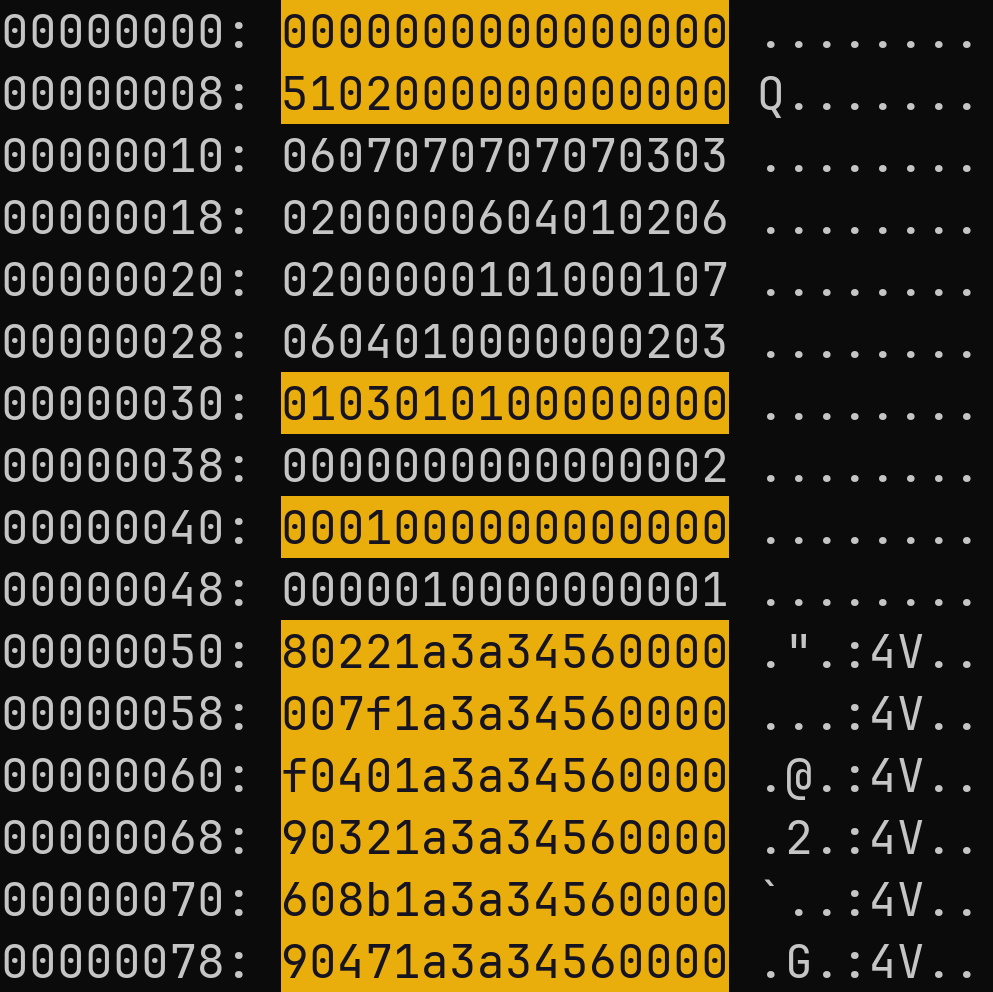
\includegraphics[width=16cm]{dataset/pointer_examples_1010-1644391327-heap_potential_pointer_highlight.png}

    We have information about the starting address of the heap using \lstinline[style=json]!"HEAP_START": "56343a198000"!. Considering that the example heap dump file contains $ 135169 $ bytes, this means that for this given heap dump file, the pointer addresses range from value $ 94782313037824_{10} $ and $ 94782313172993_{10} $. Note that the little-endian hexadecimal representation of the heap end address is \lstinline[language=c]!0x01901b3a3456! which is 12 character long, or 6 bytes long.

    Note that conversions here can get confusing, since potential pointer strings extracted from the heap dump file are given in little-endian hexadecimal format, but the heap start address from the JSON annotation file is given in big-endian hexadecimal format.

    \begin{minipage}{\dimexpr\linewidth-20pt}
        That way, we can refine the detection of potential pointers by only considering the bytes that are in the range of the heap. Potential pointers are highlighted with "<<<" in the following hex dump:

        \begin{lstlisting}[language=python, caption={Conversions function from hex strings to decimal $ int $ values}.]
        # conversion from hex to decimal
        def hex_str_to_int(hex_str: str) -> int:
            """
            Convert a normal (big-endian) hex string to an int.
            WARNING: HEAP_START in JSON is big-endian.
            """
            bytes_from_str = bytes.fromhex(hex_str)
            return int.from_bytes(
                bytes_from_str, byteorder='big', signed=False
            )
        
        def pointer_str_to_int(hex_str: str) -> int:
            """
            Convert a pointer hex string to an int.
            WARNING: Pointer hex strings are little-endian.
            """
            bytes_from_str = bytes.fromhex(hex_str)
            return int.from_bytes(
                bytes_from_str, byteorder='little', signed=False
            )
        \end{lstlisting}
    \end{minipage}

    Using the functions above, we can check which potential pointers are indeed within the heap dump range.

    \begin{minipage}{\dimexpr\linewidth-20pt}
        That way, we can refine the detection of potential pointers. In the following, pointers are highlighted with \lstinline[style=hexdump]!<<<! in the following hex dump:

        \begin{lstlisting}[style=hexdump, caption={8 bytes per line visualization of a Hex Dump from \textit{Training/basic/V\_7\_8\_P1/16/5070-1643978841-heap.raw}}]
            00000000: 0000000000000000 ........
            00000008: 5102000000000000 Q.......
            00000010: 0607070707070303 ........
            00000018: 0200000604010206 ........
            00000020: 0200000101000107 ........
            00000028: 0604010000000203 ........
            00000030: 0103010100000000 ........
            00000038: 0000000000000002 ........
            00000040: 0001000000000000 ........
            00000048: 0000010000000001 ........
            00000050: 80221a3a34560000 .".:4V.. <<<
            00000058: 007f1a3a34560000 ...:4V.. 
            00000060: f0401a3a34560000 .@.:4V.. <<<
            00000068: 90321a3a34560000 .2.:4V.. <<<
            00000070: 608b1a3a34560000 `..:4V.. <<<
            00000078: 90471a3a34560000 .G.:4V.. <<<
        \end{lstlisting}
    \end{minipage}

    \begin{minipage}{\dimexpr\linewidth-20pt}
        One last check we can do, is verify if the potential pointers are  8-bytes aligned. This can be done by checking if the last 3 bits of the potential address are 0, or using a modulo 8 operation. A simple python function can be used to check that:

        \begin{lstlisting}[language=python, caption={Python function to check if a potential pointer is 8-bytes aligned}]
            def is_pointer_aligned(pointer: int) -> bool:
                """
                Check if a pointer is 8-bytes aligned.
                """
                return pointer % 8 == 0
        \end{lstlisting}
    \end{minipage}

    Using this function on the potential pointers we have found so far, we can see that all of them are indeed 8-bytes aligned. This is a good sign for pointer detection, as we now have a range of tests that can be used to detect potential pointers from other potentially random values.

    Here is the pseudo-code for the pointer detection algorithm. This algorithm is presented for a full heap dump file:

    \begin{algorithm}
        \caption{Pointer Detection Algorithm}
        \begin{algorithmic}[1]
        \Procedure{PointerDetection}{$\text{heapDumpFile, HEAP\_START}$}
            \State $\text{heapStart} \gets \text{hex\_str\_to\_int}(HEAP\_START)$
            \State $\text{heapEnd} \gets \text{heapStart} + \text{FileSize}(\text{heapDumpFile})$
            \State $\text{position} \gets 0$
            \State $\text{potentialPointers} \gets []$
            \While{$\text{position} < \text{FileSize}(\text{heapDumpFile})$}
                \State $\text{block} \gets \text{Read8Bytes}(\text{heapDumpFile, position})$
                \If{$\text{block} \neq 0$}
                    \State $\text{pointer} \gets \text{pointer\_str\_to\_int}(\text{block})$
                    \If{$\text{heapStart} \leq \text{pointer} \leq \text{heapEnd}$}
                        \If{$\text{is\_pointer\_aligned}(\text{pointer})$}
                            \State $\text{Append}(\text{pointer}, \text{potentialPointers})$
                        \EndIf
                    \EndIf
                \EndIf
                \State $\text{position} \gets \text{position} + 8$
            \EndWhile
            \State \Return $\text{potentialPointers}$
        \EndProcedure
        \end{algorithmic}
    \end{algorithm}

    This pseudo-code outlines the steps for detecting potential pointers in the heap dump file. It starts by reading the heap dump file 8 bytes at a time. For each 8-byte block, it checks if the block is non-zero and within the heap range. If so, it checks if the potential pointer is 8-bytes aligned using the \texttt{is\_pointer\_aligned} function we described before. If all conditions are met, the potential pointer is added to the list of potential pointers. The algorithm returns this list at the end.
    
    \subsubsection{Detecting potential keys}
    % speak about SmartKex22 brute force approach
    % describe the algorithm to detect potential keys

    Encryption key prediction is the main focus of the present thesis. As such, we will now focus on how to detect potential keys in heap dump files. The paper \citetitle{SmartKex22} introduces 2 algorithms for key detection. The first one is a brute force approach that consists in trying all the possible keys in the heap dump file. The second one is a more sophisticated approach that uses a set of rules to detect potential keys.
    
    The first brute-force algorithm is given by:

    \begin{algorithm}[H]
    \caption{SSH keys brute-force algorithm from \citetitle{SmartKex22} \cite{SmartKex22}}
    \begin{algorithmic}[1]
    \Procedure{FindIVAndKey}{$\text{netPacket}, \text{heapDump}$}
        \State $\text{ivLen} \gets 16$ \Comment{Based on the encryption method}
        \State $\text{keyLen} \gets 24$ \Comment{Based on the encryption method}
        \State $i \gets \text{sizeof(cleanHeapDump)}$
        \State $r \gets 0$
        \While{$r < i$}
            \State $\text{pIV} \gets \text{heapDump}[r : r + \text{ivLen}]$
            \State $x \gets 0$
            \While{$x < i$}
                \State $\text{pKey} \gets \text{heapDump}[x : x + \text{keyLen}]$
                \State $f \gets \text{decrypt}(\text{netPacket}, \text{pIV}, \text{pKey})$
                \If{$f$ is TRUE}
                    \State \textbf{return} $\text{pIV}, \text{pKey}$
                \EndIf
                \State $x \gets x + 8$ \Comment{The IV is 8-bytes aligned}
            \EndWhile
            \State $r \gets x + 8$ \Comment{The key is 8-bytes aligned}
        \EndWhile
    \EndProcedure
    \end{algorithmic}
    \end{algorithm}
    
    Algorithm~1 outlines the brute-force approach for finding the Initialization Vector (IV) and the key. Initially, the lengths \(\text{ivLen}\) and \(\text{keyLen}\) are set based on the encryption method used for the heap. The algorithm then takes the first \(\text{ivLen}\) bytes from the heap dump to serve as the potential IV (\(pIV\)). Subsequently, \(\text{keyLen}\) bytes are extracted from the heap dump, starting from the first byte, to act as the potential key (\(pKey\)). The algorithm iterates through this potential key until it reaches the end of the heap dump. If decryption of the network packet is unsuccessful, the process is repeated by reading the next potential IV and the subsequent potential key \cite{SmartKex22}. 

    This algorithm is fairly straightforward, and can be implemented in a few lines of code. However, it is also very inefficient, as it tries all the possible keys in the heap dump file. It also needs some encrypted network packets to be able to test the keys, which are not included in the dataset. As such, we will not implement this algorithm.
    
    This is why the authors of the paper have also developed a more sophisticated algorithm that uses a set of rules to detect potential keys.

    No pseudo-code is given for the second algorithm, but the paper \citetitle{SmartKex22} gives a description of the algorithm. It rely on the high-entropy assumption of encryption keys. The algorithm is inspired by image processing techniques, and can be described as follows:

    \begin{algorithm}
        \caption{Image-processing inspired Preprocessing Algorithm, as described in \citetitle{SmartKex22} \cite{SmartKex22}}
        \begin{algorithmic}[1]
        \Procedure{Preprocessing}{$\text{heapData}$}
            \State \textbf{Reshape} $\text{heapData}$ into $N \times 8$ matrix $X$
            \For{$i = 0$ to $N-1$}
                \For{$j = 0$ to $7$}
                    \State $Y[i][j] = |X[i][j] - X[i][j+1]| \& |X[i][j] - X[i+1][j]|$
                    \State $Z[i] = \text{count}(Y[i][k] == 0) \geq 4$
                    \If{$i < N-1$}
                        \State $R[i] = Z[i] \& Z[i+1]$
                    \EndIf
                \EndFor
            \EndFor
            \State \textbf{Extract} 128-byte slices from $R$ for training
        \EndProcedure
        \end{algorithmic}
    \end{algorithm}
    
    This Preprocessing Algorithm serves as a crucial step in adapting the heap data for machine learning models. The algorithm begins by reshaping the raw heap data into an \(N \times 8\) matrix \(X\), since keys are 8-bytes aligned \cite{SmartKex22}. Here, \(N \times 8\) is the size of the original heap data in bytes. It then calculates the discrete differences of the bytes in both vertical and horizontal directions, storing the results in matrix \(Y\). The algorithm employs a logical AND operation on these differences to identify high-entropy regions, which are likely candidates for encryption keys. Each 8-byte row in \(Y\) is examined for randomness, and if at least half of its bytes differ from adjacent bytes, it is marked as a potential part of an encryption key. The algorithm then filters out isolated rows that are unlikely to be part of an encryption key, resulting in an array \(R\). Finally, 128-byte slices are extracted from \(R\) for training the machine learning model. This preprocessing step not only adapts the data for machine learning but also narrows down the search space for potential encryption keys, thereby enhancing the efficiency of the subsequent steps. 

    However, this algorithm is not as efficient as it could be. It rely on using a kind of sliding window, which is not easily parallelizable. Also, the entropy-inspired computation is not as straightforward as it could be. That why we propose a new algorithm that is more efficient and more easily parallelizable.

    In order to perform some \acrshort{ml} techniques, and because the keys we are looking for can have a range of possible lengths (16, 24, 32, or 64 bytes), we shift the focus from detecting the full key, to just be able to predict the address of the key. That way, we can deal with keys of different sizes, and we can also use the same algorithm to detect the IV. This is why we will focus on detecting potential keys addresses, and not the full keys.

    We thus introduce a new algoritm for narrowing the search space for potential keys. This algorithm is inspired by the paper \citetitle{SmartKex22}, but is more efficient and more easily parallelizable, as it focuses on producing pairs of blocks of 8 bytes with high entropy. It uses directly the Shannon entropy formula, with each entropy computation being independent from the others.

    \begin{algorithm}
        \caption{Entropy Based Detection of Potential Key blocks}
        \begin{algorithmic}[1]
        \Procedure{EntropyDetection}{$\text{heapData}$}
            \State \textbf{Pad} $\text{heapData}$ with 0s to be 8-bytes aligned
            \State \textbf{Reshape} $\text{heapData}$ into $N \times 8$ matrix $X$
            \For{$i = 0$ to $N-1$,}
                \State $entropy[i] = \text{ShannonEntropy}(X[i])$ \Comment{Independents, compute in parallel.}
            \EndFor
            \State \textbf{Add} $entropy$ 2 by 2 pairs into $entropy\_pairs$ \Comment{Keep block indexes in resulting tuples.}
            \State \textbf{Sort} $entropy\_pairs$ by entropy as $sorted\_pairs$
            \State \Return $\text{SortedPairs}(\text{sorted\_pairs})$
        \EndProcedure
        \end{algorithmic}
    \end{algorithm}

    The \textit{Entropy Based Detection of Potential Key blocks} algorithm takes a raw heap dump, represented by the variable \texttt{heapData}, as input. The data is first padded with zeros to align it to 8-byte blocks and then reshaped into an $N \times 8$ matrix $X$. The Shannon entropy is computed for each 8-byte block in parallel, resulting in an array \texttt{entropy}. Subsequently, the entropy values of adjacent blocks are summed to form pairs, which are stored in \texttt{entropy\_pairs} along with their block indexes. These pairs are then sorted by their entropy sums to produce \texttt{sorted\_pairs}. The idea of using pairs of blocks instead of a single block or more that two blocks is related to the minimim key size, which is 16 bytes. This means that we need at least 2 blocks to be able to detect a potential key. The algorithm returns sorted pairs, so that we can easily extract the ones with the highest entropy sums. Given the index of a block, its actual memory address can be recomputed using the \texttt{HEAP\_START} address available in annotations.
    
    Using this algorithm, let's continue to explore our example heap dump file from \ref{lst:hexdump-8bytes}. We will use the following python function to compute the Shannon entropy of a given block of 8 bytes:

    \begin{minipage}{\dimexpr\linewidth-20pt}
    \begin{lstlisting}[language=python, caption={Python function to compute the Shannon entropy of a given block of 8 bytes}]
        def get_entropy(data: bytes):
            """
            Computes the entropy of a byte array, using Shannon's formula.
            """

            if len(data) == 0:
                return 0.0
            
            # Count the occurrences of each byte value
            _, counts = np.unique(data, return_counts=True)
            
            # Calculate the probabilities
            prob = counts / len(data)
            
            # Calculate the entropy using Shannon's formula
            entropy = -np.sum(prob * np.log2(prob))
            
            return entropy
    \end{lstlisting}
    \end{minipage}

    This function used np array function for efficient computation. We can now use this function to compute the entropy of each block of 8 bytes in the heap dump file. We can then sort the pair of blocks by their entropy, and keep the ones with the highest entropy.
    
    When applied to the file \textit{Training/basic/V\_7\_8\_P1/16/5070-1643978841-heap.raw}, the algorithm produced $ 16896 $ entropy pairs, with $ 631 $ pairs having the maximum entropy sum. Another test using the index to address conversion and the JSON annotation file also indicate that all of the 6 key addresses are within the $ 631 $ pairs with the highest entropy sum.
    
    This allows to reduce significantly the search space for potential keys, to already less that 4\% of the original heap dump file, which is significantly better that the 30\% reduction obtained by the preprocessing algorithm described in the paper SmartKex \cite{SmartKex22}, but less that the 2\% reduction obtained by the \acrshort{ml}-based processing algorithm described in the paper \cite{SmartKex22}. However the same paper indicated that it was tested only for Key A and Key C, whereas this algorithm is tested for all the keys. Keep in mind that this is just an example for a single random file in the dataset, as a way to introduce the subject. In-depth experiments will be done in the dedicated chapter on \acrlong{ml}.

    Indeed, it is important to mention that we can rely on the JSON annotation files for providing labelling for key address prediction. Using this, we do not need to decrypt the network packets to be able to train our \acrshort{ml} models. This is a huge advantage, and is also required since we don't have the encrypted network packets in the dataset. Since we don't have those, and since the keys are already given, that is why we will focus on key address prediction, and not on key prediction.

    \subsection{Data structure exploration}
    Since the dataset contain whole heap dump file, we can also try to detect allocated chunks in those heap dumps. This can be done by looking for patterns in the heap dump file, in a similar fashion as we have done for potential pointers. However for data structure, we can rely on our knowledge of the C library used to know exactly what to look for.
    
    Since OpenSSH is written in C, we can expect to find some C memory chunks in the heap dump files. C uses the \lstinline[language=c]|malloc| function to allocate memory. This function is used to allocate memory for a given data structure. It takes as input the size of the data structure to allocate, and returns a pointer to the allocated memory. We know that the dataset has been produced using \texttt{GLIBC 2.28} \ref{sec:methods:dataset:production_system_information}. Looking directly at the code for \lstinline[language=c]|malloc| in \texttt{GLIBC 2.28}, we can read in the comments that \say{Minimum overhead per allocated chunk: 4 or 8 bytes. Each malloced chunk has a hidden word of overhead holding size and status information} \cite{MallocGLIBC2001}. This is what we refer to as the \textit{malloc header}. This means that we can expect to find some 8-bytes aligned blocks in the heap dump file, that are not pointers, but that are the result of a \lstinline[language=c]|malloc| call. Detecting and using those \textit{malloc headers} is how we will try to detect memory chunks in heap dump files.

    In Linux on a \texttt{x86\_64} architecture, the malloc function typically uses a block (chunk) header to store metadata about each allocated block. This header is placed immediately before the block of memory returned to the user. The exact layout can vary depending on the implementation of the C library (e.g., glibc, musl), but generally, it contains the following:

    \begin{itemize}
        \item \textbf{Size of the Block}: The size of the allocated block, usually in bytes. This size often includes the size of the header itself and may be aligned to a multiple of 8 or 16 bytes.
        \item \textbf{Flags}: Various flags that indicate the status of the block, such as whether it is free or allocated, or whether the previous block is free or allocated. These flags are often stored in the least significant bits of the size field, taking advantage of the fact that the size is usually aligned, leaving the least significant bits zeroed.
    \end{itemize}

    \subsubsection{How \texttt{malloc} handles Heap Allocation}

    The \texttt{malloc} function in GLIBC 2.28 uses a boundary tag method to manage chunks of memory. Each chunk contains metadata that helps in the allocation and deallocation of memory \cite{MallocGLIBC2001} \cite{MallocInternalsWiki2023}. Below are the key components of a chunk:

    A chunck is a contiguous section of memory, in our case composed of several blocks of 8 bytes, that is handled by \texttt{malloc}. It contains the following components \cite{MallocInternalsWiki2023} \cite{StackExchangeMalloc2023}:

    \begin{enumerate}
        \item \textbf{Size of Previous Chunk}: This field exists only if the previous chunk is unallocated and its \texttt{P} (PREV\_INUSE) bit is clear. It helps in finding the front of the previous chunk.
        
        \item \textbf{Size of Chunk}: This field contains the size of the chunk in bytes along with three flags: \texttt{A} (NON\_MAIN\_ARENA), \texttt{M} (IS\_MMAPPED), and \texttt{P} (PREV\_INUSE). These flags are in the last 3 \acrshort{lsb}s of the size field. This precise block is considered in the following report as the \textit{malloc header} block. Note that the size of the chunk include the size of the \textit{malloc header}, chunk user data and \textit{footer} blocks.
        
        \item \textbf{User Data}: This is the actual memory space that is returned to the user.
        
        \item \textbf{Footer}: This is the same as the size of the chunk but is used for application data. Depending on how the chunk is represented, this is exactly the same as the \textbf{Size of Chunk} field. This is a more intuitive representation and is the one choosen in the schematical representation below.
        
        \item \textbf{Flags}:
        \begin{itemize}
            \item \texttt{A} (NON\_MAIN\_ARENA): Indicates if the chunk is in the main arena or a thread-specific arena.
            \item \texttt{M} (IS\_MMAPPED): Indicates if the chunk is allocated via \texttt{mmap}.
            \item \texttt{P} (PREV\_INUSE): Indicates if the previous chunk is in use. If false, it means the previous chunk is free.
        \end{itemize}
    \end{enumerate}

    The chunck allocation process involves the following concepts: 

    \begin{enumerate}
        \item \textbf{Initialization}: The very first chunk allocated always has the \texttt{P} bit set to prevent access to non-existent memory.
        
        \item \textbf{Free Chunks}: Free chunks are stored in circular doubly-linked lists. They contain forward and backward pointers to the next and previous chunks in the list.
        
        \item \textbf{Mmapped Chunks}: These chunks have the \texttt{M} bit set in their size fields and are allocated one-by-one.
        
        \item \textbf{Fastbins}: These are treated as allocated chunks and are consolidated only in bulk. These \textit{bins} are used to speed up the allocation process.
        
        \item \textbf{Top Chunk}: This is a special chunk that always exists. If it becomes less than \texttt{MINSIZE} bytes long, it is replenished.
    \end{enumerate}

    As explained directly in the code comments, an allocated chunck of 8 byte blocks can be described by the diagram below \cite{MallocGLIBC2001}. Note that is representation is personal to better suit the needs of our forensic annalysis. The slight difference resides in the fact that the \texttt{footer} with the size of the considered chunk is represented as being part of the next chunk and not the current chunk. The footer of the previous chunk is actually the \texttt{mchunkptr} address. As stated in the GlicC wiki: \say{within the malloc library, a "chunk pointer" or \texttt{mchunkptr} does not point to the beginning of the chunk, but to the last word in the previous chunk - i.e. the first field in mchunkptr is not valid unless you know the previous chunk is free} \cite{MallocInternalsWiki2023}. Due to consideration of free/allocated chunks, it's actually easier to just consider the footer as being part of the next chunk, and not the current chunk. This is why the diagram below is slightly different from the one in the GLIBC wiki. This is just a difference in schematical representation, and does not change the actual data structure.

    \begin{figure}[H]
    \centering
    \begin{tikzpicture}[scale=0.99, every node/.style={scale=0.8}]
        % image from (0,0) to (16,12)
        
        % Draw rectangles
        \draw (4,1) rectangle (12,2);
        \draw (4,2) rectangle (12,3); % chunk-> Size of previous chunk
        \draw (4,3) rectangle (12,4); % malloc header (size of chunk)
        \draw (4,4) rectangle (12,5); %  mem-> user data starts here
        \draw (4,5) rectangle (12,6);
        \draw (4,6) rectangle (12,7);
        \draw (4,7) rectangle (12,8);
        \draw (4,8) rectangle (12,9); % nextchunk-> (app size of chunk)
        \draw (4,9) rectangle (12,10); % Size of next chunk
        \draw (4,10) rectangle (12,11);

        \draw[dashed] (3,3) rectangle (13,9);
        
        % after the rectangle step, the coordinates of the y axis are reversed ???
        % Dotted lines for user data
        \draw[dotted] (0,8) -- (16,8);
        \draw[dotted] (0,4) -- (16,4);

        % Dotted lines for memory band of 8 byte blocks
        \draw[dashed] (4,0) -- (4,12);
        \draw[dashed] (12,0) -- (12,12);
        
        % Labels
        \node[anchor=west] at (0,9.5) {-last-footer-};
        \node[anchor=west] at (0,8.5) {-malloc-header-};
        \node[anchor=west] at (0,7.5) {-chunk-user-data-};
        \node[anchor=west] at (0,3.5) {-chunk-footer-};
        \node[anchor=west] at (0,2.5) {-next-malloc-header-};

        \node[anchor=west] at (14,8.5) {in-use chunk};
        
        % Text inside rectangles
        \node[text width=14cm, align=center] at (8,9.5) {Size of previous chunk. If unallocated, next P=0};
        \node[text width=14cm, align=center] at (8,8.5) {Malloc header block: Size of chunk, in bytes |A|M|P};
        \node[text width=14cm, align=center] at (8,7.5) {User data starts here...};
        \node[text width=14cm, align=center] at (8,3.5) {(size of chunk, but used for application data)};
        \node[text width=14cm, align=center] at (8,2.5) {Size of next chunk, in bytes |A|0|1};
    \end{tikzpicture}
    \caption{Diagram of an allocated chunk in GLIBC 2.28 \cite{MallocGLIBC2001}.}
    \label{fig:allocated_chunk}
    \end{figure}

    The \texttt{malloc} function in GLIBC 2.28 uses a boundary tag method to manage chunks of memory. Each chunk contains metadata that helps in the allocation and deallocation of memory \cite{MallocGLIBC2001} \cite{MallocInternalsWiki2023}. The library stores available free chunks in circular doubly-linked lists called \say{bins}. This allows to quickly find a free chunk of memory of a given size. The problem is that we don't have access to those bins in the heap dump file. So to detect if a given chunk is in-use or free, we can rely on several methods. The first one is to look at the \texttt{P} bit of the malloc header. If it is set to 1, it means that the chunk is in use. If it is set to 0, it means that the chunk is free. 

    I also remarked that sometimes, the given heap dump file is cropped and the last block is only composed of zeros and not complete. This is for instance the case with the last chunk of \textit{Training/basic/V\_7\_1\_P1/24/17016-1643962152-heap.raw}.

\begin{lstlisting}[language=bash, caption={Logs from chunk exploration script, related to the last chunk of the file \textit{Training/basic/V\_7\_1\_P1/24/17016-1643962152-heap.raw}. }]
WARN: Chunk [94022266975200] Chunk(block_index=10876, size=48176, flags=[A=False, M=False, P=True]) is out of bounds. Last block index: 16895 Iteration index: 16896 
WARN: Chunk [94022266975200] Chunk(block_index=10876, size=48176, flags=[A=False, M=False, P=True]) is out of bounds. Last block index: 16895 Iteration index: 16897
Chunk(block_index=10876, size=48176) is only composed of zeros.
\end{lstlisting}

    A free chunk contains the pointers of the next and previous free chunks in the heap, for its given bin. A representation of a free chunk, based directly on the code documentation \cite{MallocGLIBC2001}, is given below:

    \begin{figure}[H]
        \centering
        \begin{tikzpicture}[scale=0.99, every node/.style={scale=0.8}]
            % image from (0,0) to (16,12)
            
            % Draw rectangles
            \draw (4,1) rectangle (12,2);
            \draw (4,2) rectangle (12,3); % chunk-> Size of previous chunk
            \draw (4,3) rectangle (12,4); % malloc header (size of chunk)
            \draw (4,4) rectangle (12,5); %  mem-> user data starts here
            \draw (4,5) rectangle (12,6);
            \draw (4,6) rectangle (12,7);
            \draw (4,7) rectangle (12,8);
            \draw (4,8) rectangle (12,9); % nextchunk-> (app size of chunk)
            \draw (4,9) rectangle (12,10); % Size of next chunk
            \draw (4,10) rectangle (12,11);
    
            \draw[dashed] (3,3) rectangle (13,9);
            
            % after the rectangle step, the coordinates of the y axis are reversed ???
            % Dotted lines for user data
            \draw[dotted] (0,8) -- (16,8);
            \draw[dotted] (0,4) -- (16,4);
    
            % Dotted lines for memory band of 8 byte blocks
            \draw[dashed] (4,0) -- (4,12);
            \draw[dashed] (12,0) -- (12,12);
            
            % Labels
            \node[anchor=west] at (0,9.5) {-last-footer-};
            \node[anchor=west] at (0,8.5) {-malloc-header-};
            \node[anchor=west] at (0,3.5) {-chunk-footer-};
            \node[anchor=west] at (0,2.5) {-next-malloc-header-};

            \node[anchor=west] at (0,7.5) {-forward-bin-pointer-};
            \node[anchor=west] at (0,6.5) {-backward-bin-pointer-};
    
            \node[anchor=west] at (14,8.5) {free chunk};
            
            % Text inside rectangles
            \node[text width=14cm, align=center] at (8,9.5) {Size of previous chunk. If unallocated, next P=0};
            \node[text width=14cm, align=center] at (8,8.5) {Malloc header block: Size of chunk, in bytes |A|0|P};
            \node[text width=14cm, align=center] at (8,7.5) {Forward pointer to next chunk in list};
            \node[text width=14cm, align=center] at (8,6.5) {Back pointer to previous chunk in list};
            \node[text width=14cm, align=center] at (8,5.5) {Unused space (may be 0 bytes long)};
            \node[text width=14cm, align=center] at (8,3.5) {(size of chunk, but used for application data)};
            \node[text width=14cm, align=center] at (8,2.5) {Size of next chunk, in bytes |A|0|0};
        \end{tikzpicture}
        \caption{Diagram of a free chunk in GLIBC 2.28 \cite{MallocGLIBC2001}.}
        \label{fig:free_chunk}
    \end{figure}

    \subsubsection{Chunk chaining}
    The chunk chaining algorithm relies on the \textbf{chunck chaining assumption} \ref{sec:methods:dataset:assumptions}. This assumption states that the allocator allocates chunks after chunks, and that the chunks are contiguous in memory. This means that we can expect to find the malloc header of the next chunk at the address $ \text{current\_malloc\_header\_chunk\_address} + \text{current\_chunk\_size} + 8 $, where 8 is the size of the malloc header block, or $ \text{current\_chunk\_user\_data\_address} + \text{current\_chunk\_size} $. This is the case for both free and allocated chunks. This is why we can use this assumption to detect chunks in the heap dump file. 
    
    This necessitates to understand malloc header blocks, and how they are represented in the heap dump file. In the specific case of \texttt{GLIBC 2.28}, the malloc header is defined as follows:

    \begin{minipage}{\dimexpr\linewidth-20pt}
        \begin{lstlisting}[language=c, caption={Malloc header definition in \texttt{GLIBC 2.28}}]
            #define SIZE_BITS (PREV_INUSE | IS_MMAPPED | NON_MAIN_ARENA)
        \end{lstlisting}
    \end{minipage}
    
    Since the malloc header respects the endianness of the system, we can expect to find the malloc header in little-endian format in the heap dump file. Using vim on \textit{Training/basic/V\_7\_8\_P1/16/5070-1643978841-heap.raw}, we can use the following command to find some potential malloc headers:

    \begin{lstlisting}[language=bash, caption={Vim command to find potential malloc headers}]
        :/[0-9a-f]\{4}0\{12}
    \end{lstlisting}
    
    This gives something like the following:

    \begin{figure}[H]
        \centering
        
\includegraphics[width=16cm]{dataset/structure_examples_1010-1644391327-heap_potential_malloc_header_highlight_heap_start.png}
        \caption{Attempt at malloc header detection in \textit{Training/basic/V\_7\_8\_P1/16/5070-1643978841-heap.raw}, at heap start.}
    \end{figure}

    Indeed, after a first zero block of 8 bytes (potential previous chunk footer), we expect a first data structure to be allocated at the start of the heap. Here this data structure is of size $ 5102000000000000_{16LE} $ (little-endian hex format) or $ 593_{10} $ bytes. The fact that it is an odd number is due to the \acrshort{lsb} being set to 1, to indicate that the preceding chunk is allocated (P flag). This means that the real size of the structure is actually $ 593_{10} - 1_{10} = 592_{10} $. This value is 8-byte aligned.

    Since we know that the allocator allocates chunks after chunks, we can expect the next chunk to be allocated at the address $ 5102000000000000_{16LE} + 592_{10} + 8_{10} = 5882193a34560000_{16LE} =  $. Note that we need to add 8 to the size to account for the malloc header block.
    
    In vim, since the address start at 0, we have to look at $ 592_{10} + 8_{10} = 258_{16} $. Let's have a look there:

    \begin{figure}[H]
        \centering
        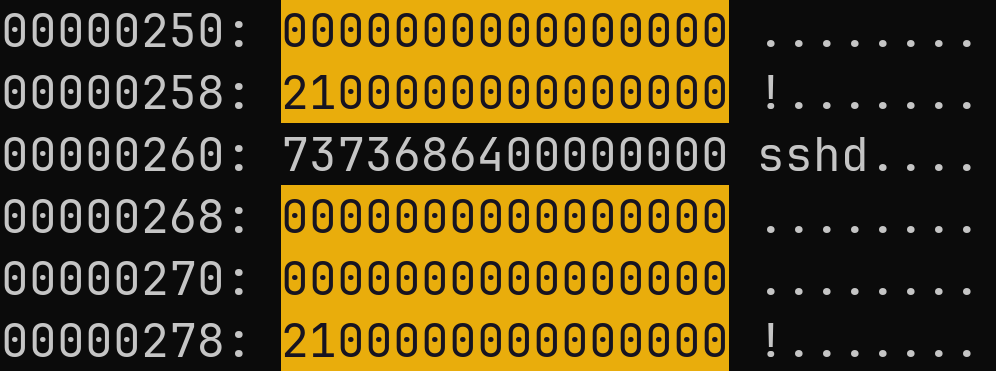
\includegraphics[width=16cm]{dataset/structure_examples_1010-1644391327-heap_potential_malloc_header_highlight_0x250.png}
        \caption{Attempt at malloc header detection in \textit{Training/basic/V\_7\_8\_P1/16/5070-1643978841-heap.raw}, at index $ 592_{10} = 250_{16} $.}
    \end{figure}

    There, we can see a zero block, followed by what we can expect to be another malloc header at address $ 258_{16} $. By doing the same process, we can thus propose an algorithm to detect the malloc headers, and thus the structures in the heap dump file.

    First, here is a simple algorithm to extract all the necessary information from a malloc header block:

    \begin{algorithm}[H]\label{alg:malloc_header_parsing}
        \caption{Malloc Header Parsing Algorithm}
        \begin{algorithmic}[1]
            \Procedure{MallocHeaderParsing}{$block$}
            \Require $block$ is a block of 8 bytes
            \Ensure $MallocHeader$ object
            \Ensure $Flags$ object
            \State \textbf{Note:} In this algorithm, $\&$ represents bitwise AND, and $\sim$ represents bitwise negation.
            \State $size\_and\_flags \leftarrow \text{ConvertBytesToInteger}(block, \text{'little-endian'})$
            \State $size \leftarrow size\_and\_flags \; \& \; (\sim 0x07)$ \Comment{Clear the last 3 bits to get the size}
            \State $Flags.a \leftarrow \text{bool}(size\_and\_flags \; \& \; 0x04)$
            \State $Flags.m \leftarrow \text{bool}(size\_and\_flags \; \& \; 0x02)$
            \State $Flags.p \leftarrow \text{bool}(size\_and\_flags \; \& \; 0x01)$
            \State \Return $MallocHeader\{size, Flags\}$
        \EndProcedure
        \end{algorithmic}
    \end{algorithm}

    We can also isolate the size parsing algorithm into a handy function:

    \begin{algorithm}[H]\label{alg:convert_to_size}
        \caption{Malloc Header block to size conversion Algorithm}
        \begin{algorithmic}[1]
            \Procedure{ConvertToSize}{$block$}
            \Require $block$ is a block of 8 bytes
            \State \textbf{Note:} In this algorithm, $\&$ represents bitwise AND, and $\sim$ represents bitwise negation.
            \State $size\_and\_flags \leftarrow \text{ConvertBytesToInteger}(block, \text{'little-endian'})$
            \State $size \leftarrow size\_and\_flags \; \& \; (\sim 0x07)$ \Comment{Clear the last 3 bits to get the size}
            \State \Return $size$
        \EndProcedure
        \end{algorithmic}
    \end{algorithm}

    Based on those algorithms, and in a similar fashion as what we have done manually by exploring the heap dump file with vim, we can propose the following algorithm to detect the malloc headers in a heap dump file:

    \begin{algorithm}[H]\label{alg:malloc_header_chaining}
        \caption{Malloc Header Chaining Algorithm}
        \begin{algorithmic}[1]
        \Procedure{MallocHeaderDetection}{$heapDumpFile$}
            \State \textbf{Note:} ConvertToSize is equivalent to MallocHeaderParsing($block$).size \Comment{See \ref{alg:convert_to_size}}
            \State \textbf{Initialize} malloc\_header\_list to empty list
            \State $position \gets 0$
            \While{$position < \text{FileSize}(heapDumpFile)$}
                \State $block \gets \text{Read8Bytes}(heapDumpFile, position)$
                \If{$\text{block} \neq 0$}
                    \State $size \gets \text{ConvertToSize}(block)$ \Comment{Be careful with flags}
                    \State \textbf{Assert} $size != 0$
                    \State \textbf{Assert} $size \mod 8 = 0$ \Comment{Check if the size is 8-bytes aligned}
                    \State $position \gets position + size$ \Comment{Leap over data structure.}
                \Else
                    \State $position \gets position + 8$
                \EndIf
            \EndWhile
            \State \Return $malloc\_header\_list$
        \EndProcedure
        \end{algorithmic}
    \end{algorithm}

    The idea behing the malloc header detection algorithm is simple. We start at the beginning of the heap dump file, and we look for the first non-zero block. We then assume that the next block is a malloc header. We convert it to a size, and then leap over the user data and the footer up to the next chunk malloc header block index. The process is repeated until reaching the end of the heap dump file.

    Note that in case of a problem, like when the size obtained from malloc header parsing is equal to 0, this means that the heap dump chaining is broken. This has been handled in the dataset cleaning section \ref{sec:methods:dataset:cleaning}. 

    \subsubsection{Chunk chaining example}
    The program \texttt{chunk\_algorithms.py} has been developped specifically to test the chunk parsing and refine the associated algorithms.

    We can test our chunk parsing algorithm on a test file in the cleaned dataset.

    \begin{lstlisting}[language=bash, caption={Testing chunk parsing on \textit{Training/basic/V\_7\_1\_P1/24/17016-1643962152-heap.raw}. Partial log output. }]
$ python src/data_structure_detection.py --input /home/onyr/code/phdtrack/phdtrack_data_clean/Training/Training/basic/V_7_1_P1/24/17016-1643962152-heap.raw --debug
    Datetime: 2023_09_27_17_08_23_157209
    Chunk [1]: Chunk(block_index=2, size=592, flags=[A=False, M=False, P=True])
    Chunk [2]: Chunk(block_index=76, size=32, flags=[A=False, M=False, P=True])
    Chunk [3]: Chunk(block_index=80, size=32, flags=[A=False, M=False, P=True])
    Chunk [4]: Chunk(block_index=84, size=32, flags=[A=False, M=False, P=True])
    Chunk [5]: Chunk(block_index=88, size=32, flags=[A=False, M=False, P=True])
    Chunk [6]: Chunk(block_index=92, size=192, flags=[A=False, M=False, P=True])
    Chunk [7]: Chunk(block_index=116, size=32, flags=[A=False, M=False, P=True])
    Chunk [8]: Chunk(block_index=120, size=32, flags=[A=False, M=False, P=True])
    Chunk [...]: ...
    Chunk [911]: Chunk(block_index=10194, size=128, flags=[A=False, M=False, P=True])
    Chunk [912]: Chunk(block_index=10210, size=256, flags=[A=False, M=False, P=True])
    Chunk [913]: Chunk(block_index=10242, size=160, flags=[A=False, M=False, P=True])
    Chunk [914]: Chunk(block_index=10262, size=512, flags=[A=False, M=False, P=True])
    Chunk [915]: Chunk(block_index=10326, size=1296, flags=[A=False, M=False, P=True])
    Chunk [916]: Chunk(block_index=10488, size=1552, flags=[A=False, M=False, P=True])
    Chunk [917]: Chunk(block_index=10682, size=1552, flags=[A=False, M=False, P=True])
    Chunk [918]: Chunk(block_index=10876, size=48176, flags=[A=False, M=False, P=True])
    -----------> Statistics:
    Total number of files: 1
    Total number of chunks: 918
    Total number of blocks: 16896
    Total number of chunks with P=1: 903
    Total number of chunks with M=1: 0
    Total number of chunks with A=1: 0
    Total number of chunks only composed of zeros: 1
    \end{lstlisting}

    Looking at the first allocated chunks, we recognize what we had seen manually with vim for the file \textit{Training/basic/V\_7\_8\_P1/16/5070-1643978841-heap.raw}. The first chunk is of size 592, and the next one is of size 32. This is exactly what we had seen manually. It is a good sign that our algorithm is working as expected. We can also see that the last chunk is of size 48176, which is significantly bigger than the other chunks. This chunk is only composed of zeros, and is truncated, meaning that its size if bigger than the actual size of the heap dump file. 
    
    \subsubsection{Distinguishing between free and allocated chunks}
    The malloc header chaining algorithm allows to detect memory chunks in the heap dump file. However, it does not allow to distinguish between free and allocated chunks. This is a problem, since we want to be able to distinguish between free and allocated chunks, to be able to detect potential data structures and filter out useless blocks.
    
    Considering the structural differences between a free and in-use block, it's possible to try distinguishing free blocks by their \textit{forward} and \textit{backward} pointers. The issue is that the head dump raw file are not provided with any \textit{bins} information. As such, distinguishing between two normal pointers and the ones expected inside a free block is a non-trivial task. Hence, the tests performed on this idea are inconclusive. A more straightforward technique is to rely on the \texttt{P} malloc header flags. 
    
    \begin{figure}[H]
        \centering
        \begin{tikzpicture}[scale=0.99, every node/.style={scale=0.8}]
            % Dotted lines for memory band of 8 byte blocks
            \draw[dashed] (4,0) -- (4,15);
            \draw[dashed] (12,0) -- (12,15);

            % ... Ellipses to represent continuation
            \node[anchor=east] at (8.5,14.5) {...in-use...};

            % Chunk - In-use
            \draw (4,13) rectangle (12,14);
            \node[anchor=west] at (0,13.5) {Chunk 0: In-use};
            \node[anchor=west] at (6.5,13.5) {header has P=1};

            % Chunk - In-use
            \draw (4,12) rectangle (12,13);
            \node[anchor=west] at (0,12.5) {Chunk 1: In-use};
            \node[anchor=west] at (6.5,12.5) {header has P=1};
            
            % Chunk - Free
            \draw (4,11) rectangle (12,12);
            \node[anchor=west] at (0,11.5) {Chunk 2: Free};
            \node[anchor=west] at (6.5,11.5) {header has P=1};

            % Chunk - In-use
            \draw (4,10) rectangle (12,11);
            \node[anchor=west] at (0,10.5) {Chunk 3: In-use};
            \node[anchor=west] at (6.5,10.5) {header has P=0};
    
            % Chunks - from top to bottom (inverted order)
            % ... Ellipses to represent continuation
            \node[anchor=east] at (8.5,9.5) {...in-use...};

            % Chunk - In-use
            \draw (4,8) rectangle (12,9);
            \node[anchor=west] at (0,8.5) {Chunk 100: In-use};
            \node[anchor=west] at (6.5,8.5) {header has P=1};
            
            % Chunk - Free
            \draw (4,7) rectangle (12,8);
            \node[anchor=west] at (0,7.5) {Chunk 101: Free};
            \node[anchor=west] at (6.5,7.5) {header has P=1};
            
            % Chunk - In-use, P=0
            \draw (4,6) rectangle (12,7);
            \node[anchor=west] at (0,6.5) {Chunk 103: In-use};
            \node[anchor=west] at (6.5,6.5) {header has P=0};
            
            % ... Ellipses to represent continuation
            \node[anchor=east] at (8.5,5.5) {...in-use...};
            
            % Chunk - In-use
            \draw (4,4) rectangle (12,5);
            \node[anchor=west] at (0,4.5) {Chunk 1000: In-use};
            \node[anchor=west] at (6.5,4.5) {header has P=1};
            
            % Chunk - Free
            \draw (4,3) rectangle (12,4);
            \node[anchor=west] at (0,3.5) {Chunk 1001: Free};
            \node[anchor=west] at (6.5,3.5) {header has P=1};
            
            % Chunk - In-use, P=0
            \draw (4,2) rectangle (12,3);
            \node[anchor=west] at (0,2.5) {Chunk 1002: In-use};
            \node[anchor=west] at (6.5,2.5) {header has P=0};

            % Chunk - In-use,
            \draw (4,1) rectangle (12,2);
            \node[anchor=west] at (0,1.5) {Chunk 1002: In-use};
            \node[anchor=west] at (6.5,1.5) {header has P=1};
            
            % ... Ellipses to represent continuation
            \node[anchor=east] at (8.5,0.5) {...in-use...};
    
        \end{tikzpicture}
        \caption{Heap dump showing a mix of free and in-use chunks. Note: each chunk immediately after a free chunk has a P flag set to 0. Each rectangle represents a chunk.}
        \label{fig:heap_dump}
    \end{figure}
    
    For a given chunk, the follow-up chunk in ascending address number, contains such a flag in its header block. If the flag value is 0, then the current chunk is free. If the flag value is 1, then the current chunk is in use by the program. This is the technique that has been used in the final implementation of the chunk chaining algorithm. 

    \begin{algorithm}[H]
        \caption{Chunk Parsing Algorithm}
        \begin{algorithmic}[1]
        \Procedure{ChunkParsing}{$heapDumpFile, HEAP\_START$}
            \State \textbf{Note:} ConvertToSize is equivalent to MallocHeaderParsing($block$).size
            \State \textbf{Note:} Get8BytesBlocks returns a list of 8 bytes blocks from the heap dump file.
            \Ensure $MallocHeader$ object
            \Ensure $Flags$ object
            \Ensure $Chunk$ object
            \Ensure $HEAP\_START$ provided from annotation file is a correct address.
            \State \textbf{Note:} In this algorithm, $\&$ represents bitwise AND, and $\sim$ represents bitwise negation.
            \State \textbf{Initialize} $chunk\_list$ to empty list
            \State $blocks \gets \text{Get8BytesBlocks}(heapDumpFile)$
            \State \textbf{Initialize} $index \gets 0$
            \While{$index < lenght(blocks)$}
                \State $block \gets blocks[index]$
                \State \textbf{Initialize} $Chunk$ to empty object
                \If{$\text{block} \neq 0$}
                    \State $Chunk.header : \{size, Flags\} \gets \text{MallocHeaderParsing}(block)$ \Comment{See \ref{alg:malloc_header_parsing}}
                    \State \textbf{Assert} $Chunk.header.size \geq 2 $ \Comment{Must contains at least header and footer}
                    \State \textbf{Assert} $Chunk.header.size \mod 8 = 0$ \Comment{Check if the size is 8-bytes aligned}
                    \State $Chunk.block\_index \gets index$ \Comment{Index of the first block of the chunk after header}
                    \State $Chunk.address \gets HEAP\_START + (index * 8)$ \Comment{Address of $block\_index$}
                    \State $footer\_index \gets index + Chunk.header.size - 1$ \Comment{Index of the footer block}
                    \If{$footer\_index < lenght(blocks)$}
                        \State $footer \gets blocks[footer\_index]$
                        \If{$\text{ConvertToSize}(footer) = Chunk.footer.size$}
                            \State $Chunk.correct_footer \gets True$
                        \Else
                            \State $Chunk.correct_footer \gets False$
                        \EndIf
                    \Else
                        \State $Chunk.correct_footer \gets False$
                    \EndIf
                    \State $next\_chunk\_header\_index \gets index + Chunk.header.size$ \Comment{Index of the next chunk header block}
                    \If{$next\_chunk\_header\_index < lenght(blocks)$}
                        \State $next\_chunk\_header \gets blocks[next\_chunk\_header\_index]$
                        \State $Chunk.is\_in\_use \gets \text{MallocHeaderParsing}(next\_chunk\_header).flags.p$
                    \Else
                        \State $Chunk.is\_in\_use \gets False$ \Comment{See \footnote{Experiments shows that last chunk can be cropped and in that case, is only composed of zeros. We can thus consider it as free.}}
                    \EndIf
                    \State $index \gets index + Chunk.header.size$ \Comment{Leap over chunk.}
                \Else
                    \State $index \gets index + 8$ \Comment{Leap over zero block.}
                \EndIf
            \EndWhile
            \State \Return $malloc\_header\_list$
        \EndProcedure
        \end{algorithmic}
    \end{algorithm}

    Note that this algorithm is based on the malloc header chaining algorithm \ref{alg:malloc_header_chaining}. The main difference is that we now have access to the malloc header flags from the following chunk, and that we can thus distinguish between free and allocated chunks. The algorithm also includes the footer parsing technique discussed briefly in the following section.

    \subsubsection{Chunk footer}
    The documentation of the \texttt{malloc} function of GLIBC  states that the footer of a chunk is the same as the size of the chunk considered. In the current report, we represent the footer as being part of the chunk itself.

    Below are two chunks content of similar size:

    \begin{lstlisting}[language=bash, caption={Printing some free and in-use chunks from \textit{Training/basic/V\_7\_1\_P1/24/17016-1643962152-heap.raw}.}]
Printing Chunk [addr:0x80a2d1438355] [status:in-use] [footer:incorrect] Chunk(block_index=80, size=32, flags=[A=False, M=False, P=True])
        Block [79]: 	b'!\x00\x00\x00\x00\x00\x00\x00' 		33 		-malloc-header-
        Block [80]: 	b'\xa0\xa2\xd1C\x83U\x00\x00' 		94022266888864 		
        Block [81]: 	b'\xc0\xa2\xd1C\x83U\x00\x00' 		94022266888896 		
        Block [82]: 	b'\x00\x00\x00\x00\x00\x00\x00\x00' 		0 		-footer-
Printing Chunk [addr:0xa09fd2438355] [status:free] [footer:correct] Chunk(block_index=8180, size=32, flags=[A=False, M=False, P=True])
        Block [8179]: 	b'!\x00\x00\x00\x00\x00\x00\x00' 		33 		-malloc-header-
        Block [8180]: 	b'\xb0\xbc\xe1\xeeS\x7f\x00\x00' 		139998466784432 		
        Block [8181]: 	b'\xb0\xbc\xe1\xeeS\x7f\x00\x00' 		139998466784432 		
        Block [8182]: 	b' \x00\x00\x00\x00\x00\x00\x00' 		32 		-footer-
    \end{lstlisting}

    Here, the status of the chunk has been detected using the \texttt{P} flag technique. At first sight, those two blocks seems similar. The first 2 blocks in the user data space of the chunks both seems to contain what look like pointers. As one can see, the first chunk in this example, with a \texttt{block\_index=80} has clearly a malloc header and footer as expected. Note that here, the value $33$ represents the size of the block ($32$ bytes which correspond to 4 blocks) with the \acrshort{lsb} being set to 1 meaning the preceding chunk is in use. However, the in-use block footer doesn't correspond to the value we expect. This difference of behavior is observed throughout the cleaned dataset. 

    \subsection{Discussing chunk parsing for problem scale reduction}
    Now that we have presented all the necessary knowledge and algorithms used to be able to parse the dataset, we can discuss the results of those algorithms and their uses and limitations. Many tests have been needed in order to develop the final algorithms. This testing process has also unveiled some interesting properties of the dataset that will be used as basis for the semantic embedding of the memory graph representation and subsequent machine learning steps.

    The program \texttt{chunk\_algorithms.py} has been developped specifically to test the chunk parsing and refine the associated algorithms on the cleaned dataset. Below are presented the global statistics produced by the final version of the program:

    \begin{lstlisting}[language=bash, caption={Printing cleaned dataset chunk parsing global statistics.}]
        Input is directory: /home/onyr/code/phdtrack/phdtrack_data_clean/
        Found 26191 files in /home/onyr/code/phdtrack/phdtrack_data_clean/.
        Processing files: 100%|\blacksquare \blacksquare \blacksquare \blacksquare \blacksquare | 26191/26191 [12:11<00:00, 35.81it/s, file=7091-1650972335]
        ------> Statistics:
        Total number of parsed files: 26191
        Total number of skipped files: 0
        Total number of chunks: 37682063
        Total number of blocks: 674232832
        Total number of chunks with P=1: 37346373
        Total number of chunks with M=1: 0
        Total number of chunks with A=1: 0
        Total number of free chunks: 354410
        Total number of chunks only composed of zeros: 18720
        Total number of blocks in free chunks: 183331224
        Total number of chunks with correct footer value: 1009522
        Total number of chunks both free and with correct footer value: 335690
        Total number of chunks free and annotated: 0
        Total number of potential footers with annotations (should be 0): 0
        Total number of annotated chunks: 209528
        Total number of chunks in used, with correct footer, and annotated: 7668
        Total number of chunks in used, with correct footer, and key annotated: 7668
        Percentage of free chunks: 0.9405270619074121%
        Percentage of blocks in free chunks: 27.19108523033183%
        Percentage of free chunks with correct footer value: 94.71798199825061%
        Percentage of in-use chunks with correct footer value: 1.8051818044922352%
        Average number of annoted chunks per file: 8.0
        Average number of chunks in use with correct footer and annotated per file: 0.2927723263716544
    \end{lstlisting}

    The cleaned dataset contains 26191 RAW files and their corresponding annotation files. The program has been able to parse all those files, and has been able to detect 37682063 chunks, which represents 674232832 blocks. This is a huge number of blocks. The goal being to be able to predict which of those blocks are first key blocks, we need to be able to filter out the useless blocks as much as possible to both optimize computations and scale down the problem. 

    Using the \texttt{P} flag technique, we can see that 37346373 chunks are in use, and 354410 chunks are free. Although the proportion of free chunks is only 0.94\%, there are 27.19\% of the blocks that are in free chunks. More importantly, we can see that no free chunk is annotated. This means we can filter out all free chunks and their blocks. This allows a huge reduction of the scale of the problem. 
    
    The average number of annotated chunks per file being a perfect 8 value, this means that all the parsed files indeed contains the 6 key annotations with the additional \texttt{SSH\_STRUCT} and \texttt{SSH\_KEY} annotations. The dataset is very imbalanced since we have only 6 keys times the number of RAW files as positive labels and the rest as negative, thus the need for advanced reduction techniques. 
    
    The exact code to annotate the chunks can be as simple as the following:

    \begin{algorithm}[H]
        \caption{Annotate Chunk Algorithm}
        \begin{algorithmic}[1]
        \Procedure{AnnotateChunk}{$chunk, keys\_addresses, ssh\_struct\_addr, session\_state\_addr$}
            \Ensure $chunk$ object
            \Ensure $keys\_addresses$ list of integers
            \Ensure $ssh\_struct\_addr$ integer
            \Ensure $session\_state\_addr$ integer
            \State \textbf{Note:} Annotations should be done after free chunk detection.
            
            \Procedure{AssertChunkUsedThenAnnotate}{$chunk, annotation$}
                \State \textbf{Assert} $chunk.is\_in\_use$ \Comment{Make sure we don't annotate free chunks}
                \State $chunk.annotations.append(annotation)$
            \EndProcedure
            
            \If{$chunk.address \in keys\_addresses$}
                \State \textsc{AssertChunkUsedThenAnnotate}($chunk, ChunkAnnotation.ChunkContainsKey$)
            \ElsIf{$chunk.address = ssh\_struct\_addr$}
                \State \textsc{AssertChunkUsedThenAnnotate}($chunk, ChunkAnnotation.ChunkContainsSSHStruct$)
            \ElsIf{$chunk.address = session\_state\_addr$}
                \State \textsc{AssertChunkUsedThenAnnotate}($chunk, ChunkAnnotation.ChunkContainsSessionState$)
            \EndIf
        \EndProcedure
        \end{algorithmic}
    \end{algorithm}
    
    This algorithm in itself and the results observed is an important discovery. The annotations are actually always given for the \texttt{chunk.address} which corresponds to the address of the first block after the malloc header block. This means that the annotations are actually given for the beginning of the user data space of a chunk. This is crucial discovery, since it means that we can filter out the malloc header and footer blocks, and only keep the first block of the user data space of the chunks we want to embed. There are $674232832 - 183331224 = 490901608$ blocks in use. But there is only $37346373$ chunks in use. This means that we can reduce the number of blocks to embed from $490901608$ to $37346373$ which is an additional reduction applied after the previous filtering that reduces the scale of the problem by a factor of 13. 
    
    Now let's look at the footer parsing. We can see in the logs that 94.72\% of free chunks are said to have a correct footer value. But this value is misleading. Since the last chunk of a heap dump is often cropped, it means it has no footer. But we consider those special last chunks as free chunks. In fact, in the $354410$ free chunks, we have $18720$ or around 5.28\% of them that are those special last cropped chunks only composed of zeros. With this perspective, we understand that 100\% of the free chunks should be considered with correct footer value. In contrast, only 1.81\% of in-use chunks have a correct footer value. It's tempting to think that maybe, those few chunks could maybe be actually empty too and removed. But this is not the case since a few chunks are actually both in-use, with a key annotation and a correct footer value. This means that we need to keep those chunks. 

    After all those extensive analysis and tests, we have gained invaluable knowledge about how we can reduce the scale of the problem and parse the files. Now, we need a way to create meaninglful embeddings for the blocks we want to perform machine learning on. This is the goal of the next section.

\section{Graph-based memory dumps embedding}\label{chap:mem_2_graph}
Now that we have a decent understanding of the dataset as well as the low level memory dump format, we can start to think about how to convert the memory dumps into graphs. As a recall, we want to be able to convert a memory dump into a graph representation that can be used for machine learning, since we want to be able to create a memory modelization as a basis for efficient embedding and feature engineering later. This is inherently due to the imbalanceness of the dataset, as we want to add more information to each memory block that just its raw bytes. The goal is to have a graph representation of the memory dump that can be used for efficient machine learning.

This section will be dedicated to describe the methods developped around this problem. We will first describe the design of the graph representation, then the implementation of the graph construction process. Finally, we will discuss the semantic embedding built from this graph representation.

\subsection{Initial work from Python to Rust}

Initially, we have been working and manipulating the code provided by SmartKex\footnote{SmartKex GitHub repository: \url{https://github.com/smartvmi/Smart-and-Naive-SSH-Key-Extraction}} for key detection. Our first explorations of the dataset quickly gave birth to some Jupyter Notebooks, which were used to explore the dataset and to understand the code, like \texttt{search\_in\_heap\_mem.ipynb}. Rapidly, we decided to rebuild a complete Python 3.11 version of the code. This was done for several reasons:

\begin{itemize}
    \item The provided code had no type hinting, which makes it hard to read and understand.
    \item We wanted to explore the dataset and learn by doing.
    \item The original code was not designed to be used as a library, but rather as a standalone script.
    \item The original code was just a few hundred lines of code and was not designed to be easily extensible, nor to be able to handle a large number of memory dumps.
    \item We wanted to modernize code by using the latest stable version of Python.
\end{itemize}

We decided to build a memory graph representation at that moment because we wanted to be able to add more information to the memory blocks than just their raw bytes. This new program was called \texttt{ssh\_key\_discover}, and relied on a number of Python libraries to work, like \texttt{graphviz}. This was a all-in-one library, composed of 2 sections, \texttt{mem\_graph} and \texttt{ml\_discovery}. The first one was devoted to build memory graphs, while the second one was dedicated to the data science and machine learning part.

This initial program was already capable of handling several data processing pipelines, including machine learning pipelines with models like Random Forest, a grid search for hyperparameter optimization, and a cross validation pipeline, several balancing strategies and of course, a memory graph representation and semantic embedding. As an early development version, this program was not optimized for performance, and just loading a given heap dump file and its annotation, and then building the memory graph representation, could take from 30 seconds to a minute (on the TUXEDO machine), depending on the size of the heap dump file. As the original dataset comprises more than $ 10^{6} $ files, a rapid estimation of the time needed just for the semantic embedding of the memory graph representation was above a month. In this regard, this initial program was just used on a bunch of files as a way to develop the semantic embedding model, algorithm and start working on feature engineering and machine learning. But it could not be used to produce final results on the whole dataset due to the performance issues described above.

This optimization issue was clearly not acceptable, and we decided to rewrite the graph part in Rust. This is a compiled language that leverages zero-cost abstractions, and thus, is several order of magnitude faster than Python. This was also a good opportunity to learn Rust, which is a language that is gaining more and more popularity, especially in the security community. This new program was called \texttt{mem2graph}. Switching from Rust to Python and doing a proper use of multithreading allowed us to reduce the time needed to build the memory graph representation from 30 seconds to less than 1 second. In out case, and comparing using only the TUXEDO laptop, this represent an estimated minimum of a 130x speedup. But this is even much better on the server, where the multithreading can really be leverage. This was a significant improvement which allowed us to build the memory graph representation for the whole original dataset in a just a few hours.

\subsection{Memory Graph Representation}
Now, let's describe the memory graph representation. The goal is to be able to represent a memory dump as a graph. This modelization makes sense since the heap dump can be considered as having memory chunks as nodes, being connected by pointers acting as arrows. This is a very natural way to represent a memory dump. However in our cases, and since the goal is to make predictions on raw bytes, we will not use the chunks as nodes, but rather the memory blocks directly. This is because we want to be able to make predictions on raw blocks of bytes, and not on chunks. 

% introduce the type of the graph, the nodes and edge
Our memory graph representation is composed of a directed graph, where each node is a memory block of bytes, and each edge is either indicative of a pointer link or a chunk membership relationship. This second representation is directly inspired by collection representation in \acrlong{kg} ontologies. In the case of \acrshort{rdf}, this could be equivalent to a \textbf{rdf:Bag}, which is an unordered container \cite{OrderedDataInRDF20} (see \ref{sec:background:ontology}). The graph is directed because the pointers are directed. We will also consider the relationship of belonging to a chunk as oriented from the data structure header block to the data structure member blocks.

Our memory graph representation is inherently a property graph. Each node and edge can have properties. The properties of an edge are the type of the edge, which can be either a pointer or a structure membership relationship.

\begin{itemize}
    \item \textbf{dts:} Data Structure Membership Relationship
    \item \textbf{ptr:} Pointer Relationship (direction is from the source to the target)
\end{itemize}

In our case, the properties of a node are at minimum the address and the byte block.  The graph is also heterogeneous since our nodes can have different types corresponding to their infered characteristics. 

\begin{itemize}
    \item \textbf{PN:} Pointer Node. This is a node whose bytes have been identified as a pointer.
    \item \textbf{DTN:} Data Structure Node. This is a node whose bytes have been identified as a data structure header. In the graph, this node is the root node of an allocated structure.
    \item \textbf{KN:} Key Node. This is a node whose bytes have been identified as a key. This identification relies both on the annotations and some verification checks.
    \item \textbf{VN:} Value Node. These are all blocks that have not been identified. It is the default  node type.
\end{itemize}

These nodes and edges form the base of the memory graph representation. Below is a simplified (truncated) example of a memory graph representation. The full example is available in \ref{appendix:mem_graph:17016-1643962152:full}. For clarity, the addresses are not displayed in this simplified version. Another version of this graph with real addresses is available in \ref{appendix:mem_graph:17016-1643962152:truncated}.

\begin{figure}[H]\label{appendix:mem_graph:17016-1643962152:simplified}
    \centering
    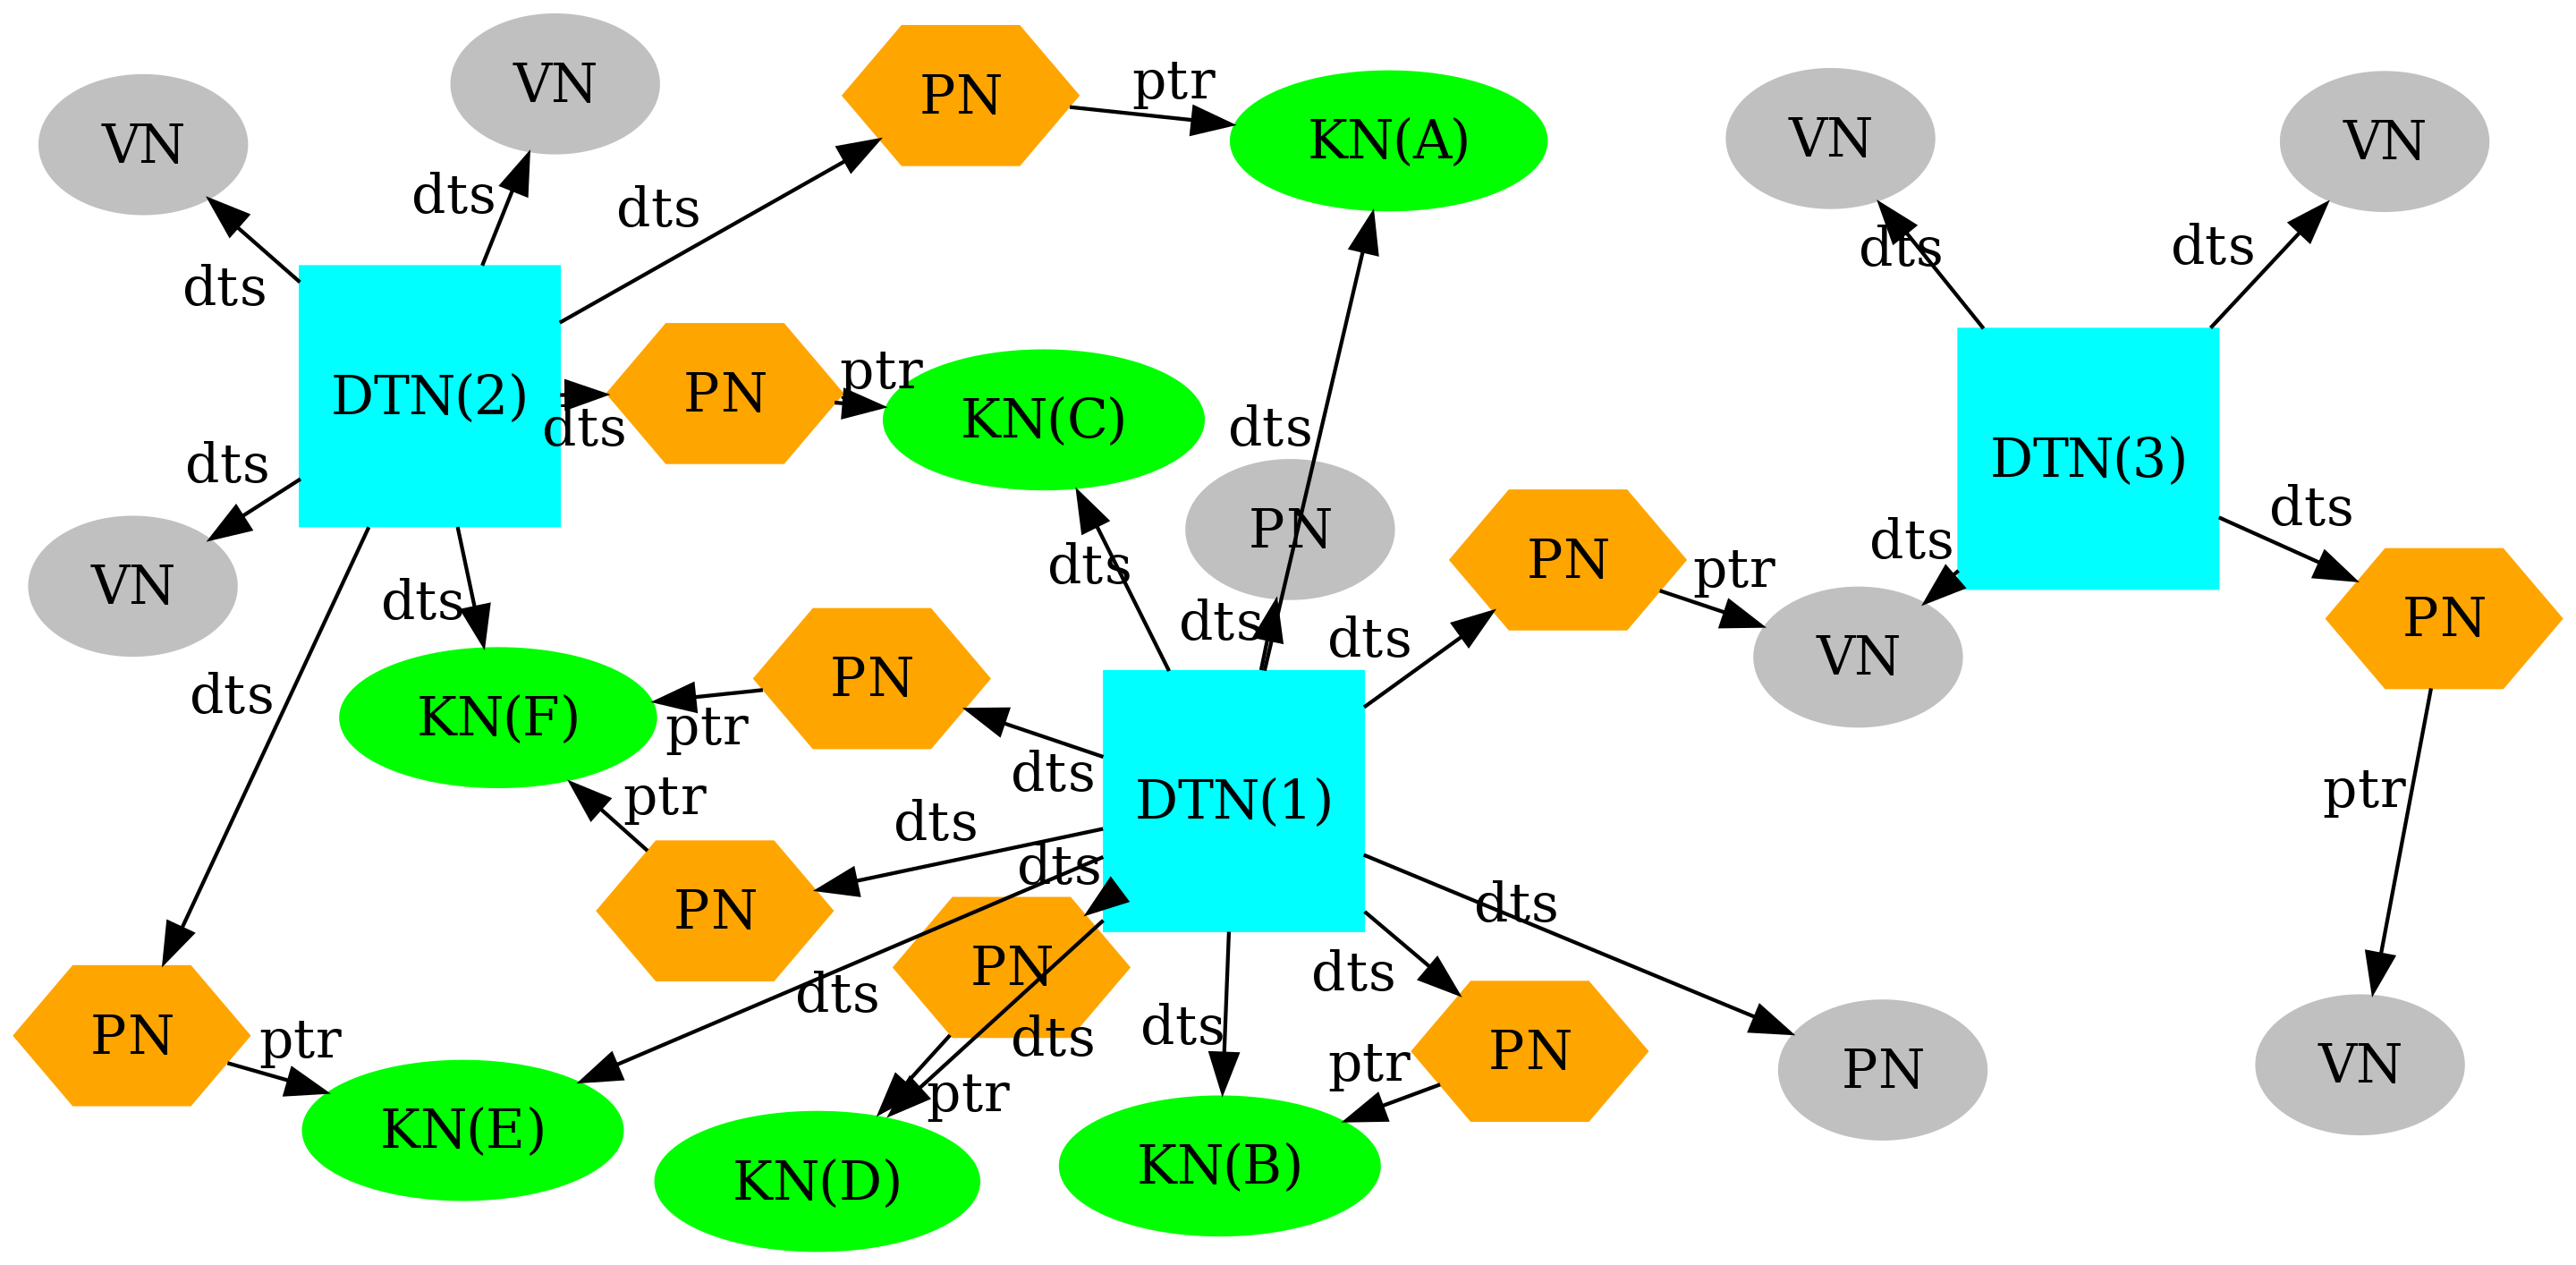
\includegraphics[width=16cm]{graphs/17016-1643962152_truncated_no_addresses.png}
    \caption{Visualization of a truncated memory graph generated from \textit{Training/basic/V\_7\_1\_P1/24/17016-1643962152-heap.raw}. The addresses are not displayed for imploved readability. Version with addresses here \ref{appendix:mem_graph:17016-1643962152:truncated}.}
\end{figure}

The given graph represents a memory layout with various types of nodes, each serving a specific purpose. The graph contains \gls{dtn} nodes, which act as the root nodes for allocated structures and are colored in cyan. These DTN nodes are connected to \gls{kn} nodes, which are identified as keys and are colored in green. The \gls{pn} nodes, colored in orange, are pointers and can be connected to value nodes or key nodes. Finally, the graph includes \gls{vn} nodes, which are the default node types and are colored in grey. These nodes have not been identified as any specific type and may contain arbitrary values.

The idea behind this representation will be to try to make predictions on the \gls{kn} nodes, which are the nodes that have been identified as keys. Using the graph, we can build an embedding of the nodes and as such, add more information to a given byte block than just its raw bytes. This is the basis of the semantic embedding, which will be discussed later.

This example is based on the heap dump file \textit{Training/basic/V\_7\_1\_P1/24/17016-1643962152-heap.raw} and has been generated using \texttt{mem2graph}, and the \textbf{sfdp} layout algorithm from \texttt{graphviz} using the following command:

\begin{lstlisting}[language=bash, caption={Command used to generate the memory graph visualization of \textit{Training/basic/V\_7\_1\_P1/24/17016-1643962152-heap.raw}}]
    sfdp -Gsize=30! -Goverlap=voronoi -Tpng 17016-1643962152_truncated_no_addresses.gv > 17016-1643962152_truncated_no_addresses.png
\end{lstlisting}

\subsection{Graph Construction}
Now that the basis of the memory graph representation has been described, let's dive in the graph construction process. 

\subsubsection{Graph Construction steps}
The graph construction process is composed of several steps:

\begin{comment}
1. graph initialization
* loading a given heap dump file and its associated annotation file
* perform some checks on the annotation file, like checking if the annotation file is valid, that all annotations are present

2. graph building
* build the graph from heap dump byte blocks
* perform data structure detection step
* perform pointer detection step

3. graph annotation
* replace VN by KN from annotation file
* add other annotations like SSH_STRUCT
After this step, its possible to export the graph to a file, like a \texttt{.dot} file or a \texttt{.gv} file for visualization or other purposes.

4. Generate embedding from graph
different embedding are possible. We will focus on the semantic embedding which is a general way to embed the graph by addind the related graph structure and vicinity information to each node.
\end{comment}

\subsubsection{Graph Construction Algorithms}


% graph construction algorithm
% graph annotation algorithm

\subsection{Exporting the Graph}
% the DOT format


\begin{minipage}{\dimexpr\linewidth-20pt}
    Here are the constants define for memory format conversion in the Rust code:

   %\begin{lstlisting}[language=json, , label={lst:json}]
   \begin{lstlisting}[style=rust, caption={Rust memory format constants in \textit{mem2graph}}]
    pub const BLOCK_BYTE_SIZE: usize = 8; // 64-bit, ex: C0 03 7B 09 2A 56 00 00
    pub const PTR_ENDIANNESS: Endianness = Endianness::Little;
    pub const MALLOC_HEADER_ENDIANNESS: Endianness = Endianness::Little;
   \end{lstlisting}
\end{minipage}

\subsection{Semantic Embedding}\label{sec:mem_2_graph:semantic_embedding}
% semantic embedding algorithm
% the CSV embedding format



%\section{Packaging and deployment with Nix}
\section{Feature engineering}
% describe the feature engineering process

\section{ML for key prediction}
% this is composed of the classical ML pipelines and of the GCN pipelines

The chapter has been an overview of the dataset, development environment, and tools used for this thesis. In the next chapter, we will dive deeper into the graph memory representation and associated algorithms and programs.


\chapter{Results}\label{chap:results}

The following section describes the experimental setup, the used and generated datasets as well as parameters to conclude with the experimental results achieved.

\section{Developped programs}
Many programs have been developped for the need of the present thesis. Early data exploration scripts have paved the way towards efficient highly parallel programs in both Rust and Python for data analysis, graph and embedding generation of ML and DL tested on different models and contexts. All the necessary concepts and methods have been introduced previously, so it is now time to present those main program in details.

\subsection{Mem2Graph}
The present report has already presented the \textit{Mem2Graph} program throughout the heap dump memory parsing algorithm, graph construction and embeddings. This program has been developped in Rust and is an active collaboration between the author and Clément Lahoche, another PhDTrack student at Passau. The program is available on GitHub at \url{https://github.com/passau-masterarbeit-2023/mem2graph}. 

The program is composed of several layers than bruild on top of each other. The first layer is dedicated into loading a RAW heap dump file with its annotation JSON file, performs some checks and prepare the data for further analysis. The next one performs the graph construction following the algorithms introduced in the Methods section. Another layer performs some annotations of the nodes. The final layer is more versatile and dependent on the input program parameters. For the need of this report, several pipelines of memgraph with and without embeddings haved been added, namely \texttt{graph} and \texttt{graph-with-embedding-comments}. The first pipeline doesn't perform any embedding and export the memory graph to a text file following the DOT format \cite{DotFormat15}. The second pipeline performs the same operations, but also exports the memory graph with the embeddings as comments in the DOT file. 

Since the prediction effort is focused on memory chunks, this embedding is generally called with the \texttt{--no-value-node} parameter, which transform the memory graph from a graph of blocks of 8 bytes, into a memory graph of memory chunks, connected by their pointers inside their respective user data space. Several chunk node embeddings have been implemented, and the user can choose which one to use. The chunk node embeddings are the following: \texttt{chunk-semantic-embedding}, \texttt{chunk-statistic-embedding}, and \texttt{chunk-start-bytes-embedding}.

\subsection{Machine Learning Pipelines Runner}

When working with machine learning, Python is a dominant language, benefiting from a rich ecosystem of libraries and frameworks.

The project leverages a wide range of Python libraries to build comprehensive machine learning pipelines:
\begin{itemize}
    \item \textit{NetworkX} for graph-based data structures and algorithms.
    \item \textit{PyGraphviz} for graph visualization.
    \item \textit{Torch} for tensor computations and building neural networks.
    \item \textit{Scikit-learn} for classical machine learning algorithms.
    \item \textit{Pandas} for data manipulation and analysis.
    \item \textit{NumPy} for numerical computations.
    \item \textit{Matplotlib} for data visualization.
    \item \textit{Torch-Geometric} for Geometric Deep Learning extensions for PyTorch.
\end{itemize}

The program encompasses a variety of machine learning models to compare how different models react to the embeddings and representations developped earlier. It includes classical machine learning models from the Scikit-learn library, such as Random Forest, Stochastic Gradient Descent (SGD), and Logistic Regression. These models serve a point of comparision since they don't rely on graph-based data structures and algorithms. 

The program also includes Graph Convolutional Network (GCN) models built on top of PyTorch and Torch-Geometric. These models are more complex and powerful, leveraging the graph structure and embeddings to achieve better results. Those models specifically leverage graph-based embeddings and input data, generated using the Node2Vec algorithm to create dense and continuous node features that can be used for subsequent analysis or machine learning tasks.

\textbf{Main Pipelines:}
The program is organized around three main pipelines:
\begin{enumerate}
    \item \textit{GCN Pipeline:} For Graph Convolutional Network models, built using libraries such as Torch and Torch-Geometric.
    \item \textit{Classical ML Pipeline:} Leveraging algorithms like Random Forest, SGD, and Logistic Regression from Scikit-learn.
    \item \textit{Feature Evaluation Pipeline:} Primarily aimed at evaluating the quality and importance of generated features or graph embeddings.
\end{enumerate}

\subsection{Other programs}
A lot of other programs have been developped for the need of this thesis, but they are not as important as the ones presented above. Those scripts and short program have been developped for several purpose:

\begin{itemize}
    \item \textbf{Data exploration:} Several scripts have been developped to explore the data, and to understand the structure of the heap dump files, the annotations, and the memory graphs.
    \item \textbf{Heap Dump parsing algorithm testers:} Several scripts have been developped to test the heap dump parsing algorithms, and to ensure that the algorithms are working as intended on all possible situations.
    \item \textbf{Graph and embedding generation testers:} Others have been developped to test the graph and embedding generation algorithms, and to ensure that the algorithms are working as intended on all possible situations.
    \item \textbf{Result visualization, analysis and latex generators:} Later in the report, the results will be presented and discussed. Several scripts have been developped to generate the latex tables and plots, and to analyze the results.
\end{itemize}

All those programs represent a consequent amount of work, and have been invaluable to the success of this thesis.

\begin{table}[h]
    \centering
    \caption{Code Statistics for Masterarbeit}
    \label{tab:cloc_output}
    \begin{tabular}{|l|r|r|r|r|}
        \hline
        Language & Files & Blank Lines & Comments & Code Lines \\
        \hline
        CSV & 867 & 0 & 0 & 158305697 \\
        Text & 25 & 272 & 0 & 50073 \\
        Python & 132 & 2326 & 2682 & 8050 \\
        Rust & 50 & 1343 & 1149 & 6823 \\
        TeX & 28 & 963 & 141 & 6636 \\
        Markdown & 33 & 1016 & 0 & 2375 \\
        JSON & 1345 & 1 & 0 & 1677 \\
        Jupyter Notebook & 2 & 0 & 1811 & 381 \\
        Nix & 12 & 50 & 31 & 290 \\
        TOML & 1 & 2 & 1 & 22 \\
        Bourne Shell & 3 & 8 & 8 & 18 \\
        make & 1 & 8 & 3 & 18 \\
        Dockerfile & 1 & 1 & 0 & 2 \\
        \hline
    \end{tabular}
\end{table}

In the context of this thesis, three programming languages stand out for their specialized roles: Python, Rust, and Nix. Python is predominantly used for the machine learning pipeline, offering ease of use and a rich ecosystem for data science tasks. Rust serves as the backbone for the Mem2Graph program, providing the efficiency required for graph construction and manipulation. Nix is employed for package management and building, ensuring reproducibility across different computing environments. These languages complement each other well, with Python offering high-level abstractions for machine learning, and Rust providing low-level control for performance-critical tasks. Additionally, CSV files are utilized to store model results. TeX is used for generating this report, highlighting the diverse yet complementary set of tools and languages employed in this research. 

\section{Experimental Setup}

The experimental setup serves as the backbone of this research, providing a structured framework for conducting large-scale experiments on the server. This section delves into the intricacies of the setup, detailing the steps involved and the tools used. It also includes selected program output logs to offer a granular view of the program parameters, environment, and usage.

The elements discussed in this section are not merely illustrative; they offer invaluable insights into the challenges encountered during the experiments. These details are particularly crucial when discussing the large-scale experiments, as they provide a comprehensive understanding of the various facets involved.

The final experiments were conducted in a systematic manner, following these steps:

\begin{enumerate}
    \item \textbf{Data Cleaning:} The original Zenodo dataset was cleaned to produce a RAW heap dump dataset, serving as the foundational data for the experiments.
    
    \item \textbf{Graph and Embedding Generation:} The Mem2Graph Rust program was employed to generate graphs along with their embeddings. A Python launcher script facilitated the generation of multiple memgraph datasets, each with varying combinations of program parameters.
    
    \item \textbf{Data Preloading and Validation:} A sanity check Python program was used for data preloading and validation, ensuring the integrity and consistency of the data before proceeding to the experimental phase.
    
    \item \textbf{ML and DL GCN Pipelines:} The main Python program was responsible for the seamless launching of data science tasks, machine learning training, and model evaluation. It was designed to cover a predefined range of parameters and model hyperparameters.
    
    \item \textbf{Result Collection and Evaluation:} The final step involved the collection, evaluation, and visualization of the results. Error handling mechanisms were in place to make necessary corrections and prepare for the next iteration of experiments. This step also facilitated the confrontation of hypotheses and research questions.
\end{enumerate}

Initial small-scale tests were conducted on a laptop to validate the programs and their results. The final, large-scale experiments were carried out on the Drogon server, equipped with 80 threads and 256GB of RAM. The computational resources provided by the University of Passau have been invaluable for conducting these experiments, sometimes running for several days straight.

\subsection{Generation of the memgraph datasets}
Using Mem2Graph powerful features, it is possible to generate several memgraph datasets with different parameters. The following command has been used to generate 6 memgraph datasets, each containing 26202 graphs, for a total of 157212 graphs. Those datasets account for different chunk node embeddings and a potential additional filtering feature. The command is run on the Drogon server, with 80 threads.

\begin{lstlisting}[language=bash, caption={Sample of final logs of the \texttt{Mem2Graph} program, after generating 6 memgraph datasets from the cleaned heap dump dataset.}, literate={_}{\_}{1}]
    [2023-10-24T20:42:44 UTC][INFO mem_to_graph::exe_pipeline::pipeline] OK [t: worker-63] [N*202 / 26202 files] [fid: 8683-1650977906]    (Nb samples: 0)
    [2023-10-24T20:42:44 UTC][INFO mem_to_graph::graph_data::heap_dump_data] FILE heap dump raw file path: "/root/phdtrack/phdtrack_data_clean/Performance_Test/V_8_1_P1/32/8794-1650977906-heap.raw"
    [2023-10-24T20:42:44 UTC][INFO mem_to_graph::exe_pipeline::pipeline] OK [t: worker-63] [N*203 / 26202 files] [fid: 8794-1650977906]    (Nb samples: 0)
    [2023-10-24T20:42:44 UTC][INFO mem_to_graph::exe_pipeline::pipeline] TIME [total pipeline time: 114.84s]
    100%|##############################| 6/6 [1:07:15<00:00, 672.62s/it]
    Finished! Total time: hours: 1, minutes: 7, seconds: 15 (Drogon Server)
\end{lstlisting}

It took a little more than an hour to generate 6 memgraph datasets, each containing 26202 graphs. The total number of graphs generated is 157212. The generated memgraph datasets are stored in the \texttt{data/} directory, as follow:

\begin{figure}[H]
    \centering
    \caption{Illustration of the Data Directory Structure}
    \label{fig:data_structure}
    \begin{minipage}{0.8\textwidth}
        \dirtree{%
            .1 /data.
            .2 0\_graph\_with\_embedding\_comments\_-v\_-a\_chunk-header-node\_-c\_chunk-semantic-embedding\_-e\_none\_-s\_none.
            .2 1\_graph\_with\_embedding\_comments\_-v\_-a\_chunk-header-node\_-c\_chunk-statistic-embedding\_-e\_none\_-s\_none.
            .2 2\_graph\_with\_embedding\_comments\_-v\_-a\_chunk-header-node\_-c\_chunk-start-bytes-embedding\_-e\_none\_-s\_none.
            .2 3\_graph\_with\_embedding\_comments\_-v\_-a\_chunk-header-node\_-c\_chunk-semantic-embedding\_-e\_only-max-entropy\_-s\_activate.
            .2 4\_graph\_with\_embedding\_comments\_-v\_-a\_chunk-header-node\_-c\_chunk-statistic-embedding\_-e\_only-max-entropy\_-s\_activate.
            .2 5\_graph\_with\_embedding\_comments\_-v\_-a\_chunk-header-node\_-c\_chunk-start-bytes-embedding\_-e\_only-max-entropy\_-s\_activate.
        }
    \end{minipage}
\end{figure}

As one can see, the dataset directory names are composed with the most important \texttt{Mem2Graph} program parameters, responsible for some feature and embedding generations. The \texttt{-e} flag, short for \texttt{--entropy-filter} is responsible for the filtering using the Shannon entropy, the \texttt{-s} for \texttt{--chunk-byte-size-filter} for chunk byte size filtering. The \texttt{-c}, \texttt{--graph-comment-embedding-type} controls the custom embedding being save alongside each node in the generated .GV memgraph files.

\subsection{Sanity checking and preloading the generated memgraph datasets}
Loading the graph from DOT files into NetworkX graph in Python is a ressource intensive operation that consumes all the available computing power on all tested platforms (laptop, servers). It takes several dozens of seconds up to a minute to load a memory graph containing only around 1000 chunk nodes. It has been experimented that saving those loaded graphs using the \textit{pickle} python library allows to perform checks while loading the graph, add more information about each graph. The subsequent retrieval of the graph is much faster, and allows to perform the sanity checks before any further processing.. So to verify the memory graph dataset generation as well as transforming DOT files into pre-saved networkx graph, a sanity checking script has been developed.

Below is a sample of the logs generated by the sanity check script:

\begin{lstlisting}[language=bash, caption={Result logs of the \texttt{memory\_graph\_gcn/src/sanity\_check\_gv\_files.py} program.}, literate={_}{\_}{1}]
    * Running program...
   Passed program params:
   param[0]: src/sanity_check_gv_files.py
   param[1]: -k
   Parsed program params:
   keep_old_output: True
   skip_dir_starting_with_number: None
   dry_run: False
    * Now, performing data loading and sanity checks...
    * Looking for Mem2Graph dataset directories in /root/phdtrack/mem2graph/data...
    * Skipping .gitignore...
    * Found 6 Mem2Graph dataset directories.
   [...]
   Loading graphs: 100%|##########| 26201/26202 [3:22:17<00:00,  1.17it/s]
   Loading graphs: 100%|##########| 26202/26202 [3:22:25<00:00,  3.19s/it]
   Loading graphs: 100%|##########| 26202/26202 [3:22:25<00:00,  2.16it/s]
    * Checking embedding length of graphs in /root/phdtrack/mem2graph/data/5_graph_with_embedding_comments_-v_-a_chunk-header-node_-c_chunk-start-bytes-embedding_-e_only-max-entropy_-s_activate...
   -> [x] 26202 graphs in /root/phdtrack/mem2graph/data/5_graph_with_embedding_comments_-v_-a_chunk-header-node_-c_chunk-start-bytes-embedding_-e_only-max-entropy_-s_activate have been loaded and checked.
   -> [_] 0 graphs in /root/phdtrack/mem2graph/data/5_graph_with_embedding_comments_-v_-a_chunk-header-node_-c_chunk-start-bytes-embedding_-e_only-max-entropy_-s_activate have been skipped (deleted).
   [x] 157212 total graphs in the input mem2graph dataset dir paths have been loaded and checked.
   [_] 0 total graphs in the input mem2graph dataset dir paths have been skipped (deleted).
   <END> Program took: 42626.062309 total sec (11h 50m 26s)
\end{lstlisting}

The sanity checking file can be considered very long to run, having taken almost 12 hours straight, but it is a necessary step to ensure the quality of the generated memgraph datasets. It is also a good way to check the validity of the generated embeddings, and to ensure that the graphs are re-exported as \texttt{NetworkX} graphs that can be loaded much faster than the original DOT files.

\subsection{Launching the experiments}
Two pass of experiments have been conducted, with the exact same parameters and input memgraph dataset. Contrary to expectations, the experiments were much faster on the laptop that on the Drogon server. 

\begin{itemize}
    \item \textbf{Time take for the experiments on the laptop:} 12h 31m 53s
    \item \textbf{Time take for the experiments on the Drogon server:} 29h 17m 57s
\end{itemize}

The experiments have been launched using the following command (here, on Drogon server):

\begin{lstlisting}[language=bash, caption={Command used to launch final experiments, on Drogon server.}, label={results:final-launching:run-experiments:command}, literate={_}{\_}{1}]
    nohup python src/main_gcn.py -i /root/phdtrack/phdtrack\_data\_clean/ -p gcn-pipeline classic-ml-pipeline feature-evaluation-pipeline -b 6 -a -q -n 16  > output\_ml\_2023\_10\_27\_16h\_35.log 2>&1 &
\end{lstlisting}
    

Using \texttt{nohup} and redirecting the output to a log file allows the experiments to run in the background and enables the retrieval of the output at a later time. The command specifies the input directory containing the annotated DOT (.gv) graph directory with the \texttt{-i} flag. All three pipelines are chosen: \texttt{gcn-pipeline}, \texttt{classic-ml-pipeline}, and \texttt{feature-evaluation-pipeline}, as indicated by the \texttt{-p} flag. The batch size for parallel processing is set to 6 using the \texttt{-b} flag, and the \texttt{-a} flag indicates the use of all available Mem2Graph datasets. The \texttt{-q} flag enables quiet mode for Node2Vec, and the \texttt{-n} flag specifies the use of 16 input graphs.

\subsection{Dealing with hyperparameter tuning}

In the quest to optimize the performance of both \acrshort{ml} and \acrshort{dl} models, hyperparameter tuning plays a crucial role. This section elaborates on the various strategies and tools employed for hyperparameter tuning in this research.

\begin{itemize}
    \item \textbf{Precise Command Lines for Tuning:} The compute instances and experiment parameters can be finely tuned using precise command-line options. This flexibility allows for a more targeted approach to model optimization, enabling the user to specify various hyperparameters and settings right from the terminal.
    
    \item \textbf{Python Program for Experiment Launch:} A dedicated Python program has been developed to automate the launching of \acrshort{ml}, \acrshort{gcn} and \acrshort{fe} pipelines. This program takes different hyperparameters as input and initiates the corresponding experiments, thereby streamlining the entire process.
    
    \item \textbf{Automatic Logging in CSV:} All the results from each experiment, along with the hyperparameters used, are automatically logged into a CSV file. This facilitates easy tracking and comparison of different model configurations and their corresponding performances.
    
    \item \textbf{Timestamps and Duration Steps:} Each experiment is meticulously logged with precise timestamps and duration steps. This includes the time taken for generating embeddings, as well as the time required for the training and testing phases. Such detailed logging aids in identifying bottlenecks and optimizing the pipeline further.
    
    \item \textbf{Extensive Experimentation:} Over the course of this research, thousands of experiments have been conducted. These experiments span a wide range of parameters, models, and embeddings, providing a comprehensive understanding of the model behaviors and their sensitivities to different hyperparameters.
    
    \item \textbf{Automated Result Analysis and Visualization:} To aid in the interpretation of the extensive experimental results, automated scripts have been developed for result analysis and visualization. These scripts generate various plots and metrics that provide insights into the performance and reliability of the different models and configurations.
\end{itemize}

Of all the parameters, the model types, their respective hyperparameters, the combinations of possible embeddings with their own parameters, and the number of input graphs are the most important. All those parameters explains the large number of experiments that have been conducted, and the need for a precise and automated way to launch them.

\subsubsection{Limited number of input graphs due to compute time and memory usage}

It also explains why the input number of memgraphs has been limited to 16, as it is already a very large number of experiments to run. Each file taking several dozens of seconds to be transformed into an embedding, this represents around 10 minutes just for the embedding generation phase, for each pipeline. With more that 600 pipelines to run, this already represents dozens of hours of compute time. Depending on the context and model, the training and evaluation phases are also time consuming, and the more input graphs there are, the longer it takes to train and test the model. 

The compute time is not the only issue with dealing with a large number of input graphs. The memory usage is also a problem, as the memory usage increases linearly with the number of input graphs. The parallel processing of only 6 pipelines having 16 memgraphs as imputs generally represents between 16 and 50 GB of RAM usage, depending on the model and the embedding used. Due to this, all tests consisting to try to run this already limited number of input graphs on the GPU have failed, as the GPU memory is not sufficient to handle the memory usage of the program. The slowness of the CPU alongside memory bandwidth limitations are the main bottlenecks of the program, and the main reasons why the number of input graphs has been limited to 16.

\subsubsection{Parallel launch of experiments}

To maximize efficiency and expedite the research process, a Python program was developed to launch multiple experiments in parallel. This approach allows for simultaneous testing of various input graphs, machine learning and deep learning models, embedding techniques, and hyperparameters. By leveraging parallel computing, the program significantly reduces the time required for extensive experimentation, thereby accelerating the overall research and development cycle.

Below are the hyperparameters used during the main experiments, as stored in the \texttt{hyperparams.json} file:

\begin{lstlisting}[style=json, caption={JSON hyperparameters used during experiments}, label={results:json-hyperparams-range}, literate={_}{\_}{1}]
        {
            "node2vec_dimensions_range": [128],
            "node2vec_walk_length_range": [16],
            "node2vec_num_walks_range": [50],
            "node2vec_p_range": [0.5, 1.0, 1.5],
            "node2vec_q_range": [0.5, 1.0, 1.5],
            "node2vec_window_range": [10],
            "node2vec_batch_words_range": [8],
            "node2vec_workers_range": [16],
            "randomforest_trees_range": [100, 500, 1000],
            "gcn_training_epochs_range": [20]
        }
\end{lstlisting}

Even though the above JSON file shows the hyperparameters selected for the large scale final experiments, pre-experiments have been previously conducted to find some eusable values. Due to compute time limitations, the ranges of hyperparameters have been limited to a few values, and the number of input graphs has been limited to 16. The following JSON file shows the hyperparameters used during the pre-experiments:

\begin{lstlisting}[style=json, caption={JSON hyperparameters used during experiments}, label={results:json-hyperparams-range}, literate={_}{\_}{1}]
    {
        "node2vec_dimensions_range": [16, 32, 128],
        "node2vec_walk_length_range": [16, 32],
        "node2vec_num_walks_range": [50, 100],
        "node2vec_p_range": [0.5, 1.0, 1.5],
        "node2vec_q_range": [0.5, 1.0, 1.5],
        "node2vec_window_range": [10, 20],
        "node2vec_batch_words_range": [4, 8, 16],
        "node2vec_workers_range": [16, 32],
        "randomforest_trees_range": [100, 500, 1000],
        "gcn_training_epochs_range": [5, 10, 20]
    }
\end{lstlisting}

Several observations were made during the early experiments concerning the impact of different hyperparameters on the model's performance, especially concerning the Node2Vec parameters. The following observations were made:

\begin{itemize}
    \item \textbf{Walk Length and Number of Walks:} Increasing the number of walks and the walk length generally improved the model's performance. However, this came at the cost of significantly increased computational time. The benefits plateaued after reaching a certain threshold.
    
    \item \textbf{Number of Dimensions:} A higher number of dimensions generally led to better results. Lower values were found to be detrimental to the model's performance, indicating the importance of this parameter.
    
    \item \textbf{Impact of \( p \) and \( q \):} The parameters \( p \) and \( q \) had an unpredictable impact on the model's performance. While some combinations seemed to yield better results, no clear pattern was observed, making these parameters challenging to optimize.
    
    \item \textbf{Batch Word Range:} The range of batch words had a minimal impact on the model's performance. As a result, an intermediate value was selected for this parameter to balance computational efficiency and performance.
\end{itemize}

These observations provide valuable insights into the behavior of the models under different hyperparameter settings and serve as a guide for future experiments.

\subsubsection{Description of the \texttt{results.csv} File}

The \texttt{*results.csv} files are used to store the results of machine learning and deep learning classifiers, including Graph Convolutional Networks (GCNs) and classical classifiers like Random Forest. The files are regular CSVs organized with the following headers:

\begin{itemize}
    \item \textbf{system}: The operating system on which the experiment was run. Here, \textit{Linux}.
    \item \textbf{node\_name}: The name of the node in the cluster. Here, either \textit{nixos} (local machine) or \textit{rascoussie} (lab server).
    \item \textbf{release, version}: OS release and version information.
    \item \textbf{machine, processor}: Hardware details.
    \item \textbf{physical\_cores, total\_cores}: Number of physical and total cores.
    \item \textbf{total\_memory, available\_memory}: Total and available memory in bytes.
    \item \textbf{start\_time}: The start time of the experiment.
    \item \textbf{nb\_input\_graphs}: Number of input graphs.
    \item \textbf{duration\_embedding}: Time taken for embedding.
    \item \textbf{subpipeline\_name, index, pipeline\_name}: Information about the pipeline model used, with values like \textit{sgd-classifier} or \textit{gcn-with-dropout}.
    \item \textbf{input\_mem2graph\_dataset\_dir\_path}: Path to the dataset directory.
    \item \textbf{node\_embedding}: Type of node embedding used. Several values are possible, like solo embeddings like \textit{chunk-header-node} or \textit{node2vec}, or combined embeddings like \textit{node2vec-chunk-semantic-embedding}.
    \item \textbf{node2vec\_*}: Parameters for the Node2Vec algorithm, like the number of walks, the walk length, the window size, the number of dimensions, the number of epochs, and the p and q parameters.
    \item \textbf{random\_forest\_*}: Parameters for the Random Forest algorithm, like the number of estimators (trees) or the number of parallel jobs.
    \item \textbf{imbalance\_ratio}: Ratio of the classes in the dataset. For instance, a value of 496.33 means that the dataset contains 496.33 times more negative samples than positive samples. Since no filtering is applied, the ratio is always greater than 1, and generally very high.
    \item \textbf{precision\_class\_*, recall\_class\_*, f1\_score\_class\_*, support\_class\_*}: Metrics for each class.
    \item \textbf{true\_positives, true\_negatives, false\_positives, false\_negatives}: Confusion matrix elements.
    \item \textbf{AUC}: Area under the ROC curve.
    \item \textbf{duration\_train\_test}: Time taken for training and testing.
    \item \textbf{nb\_node\_features}: Number of node features. This value directly depends on the node embedding used, and the input memory graph dataset parameters used during generation.
    \item \textbf{first\_gcn\_training\_epochs}: Number of epochs in GCN training phase.
\end{itemize}

Each row in the \texttt{*results.csv} files represents a single experiment run with a specific configuration and its corresponding results. Keeping a precise track of the parameters used for each experiment is crucial for reproducibility and traceability. They also form the basis for the analysis and visualization of the results.

\subsection{The challenge of ressource optimisation}

\subsection{The challenge of packet management}

\section{Obtained results on feature engineering}

\begin{lstlisting}[language=bash, caption={Command used to count the number of .gv memory graph files generated by \textit{mem2graph} inside one of the servers mem2graph dataset directory.}]
    (py311) root@compute-container-rascoussie-d584d4794-lbm9r:~/onyr_phdtrack/mem2graph# find data/ -type f -name "*.gv" | wc -l
    104808
\end{lstlisting}

\section{Feature Engineering results}

\begin{figure}[H]\label{results:corr_matrices:kendall}
    \centering
    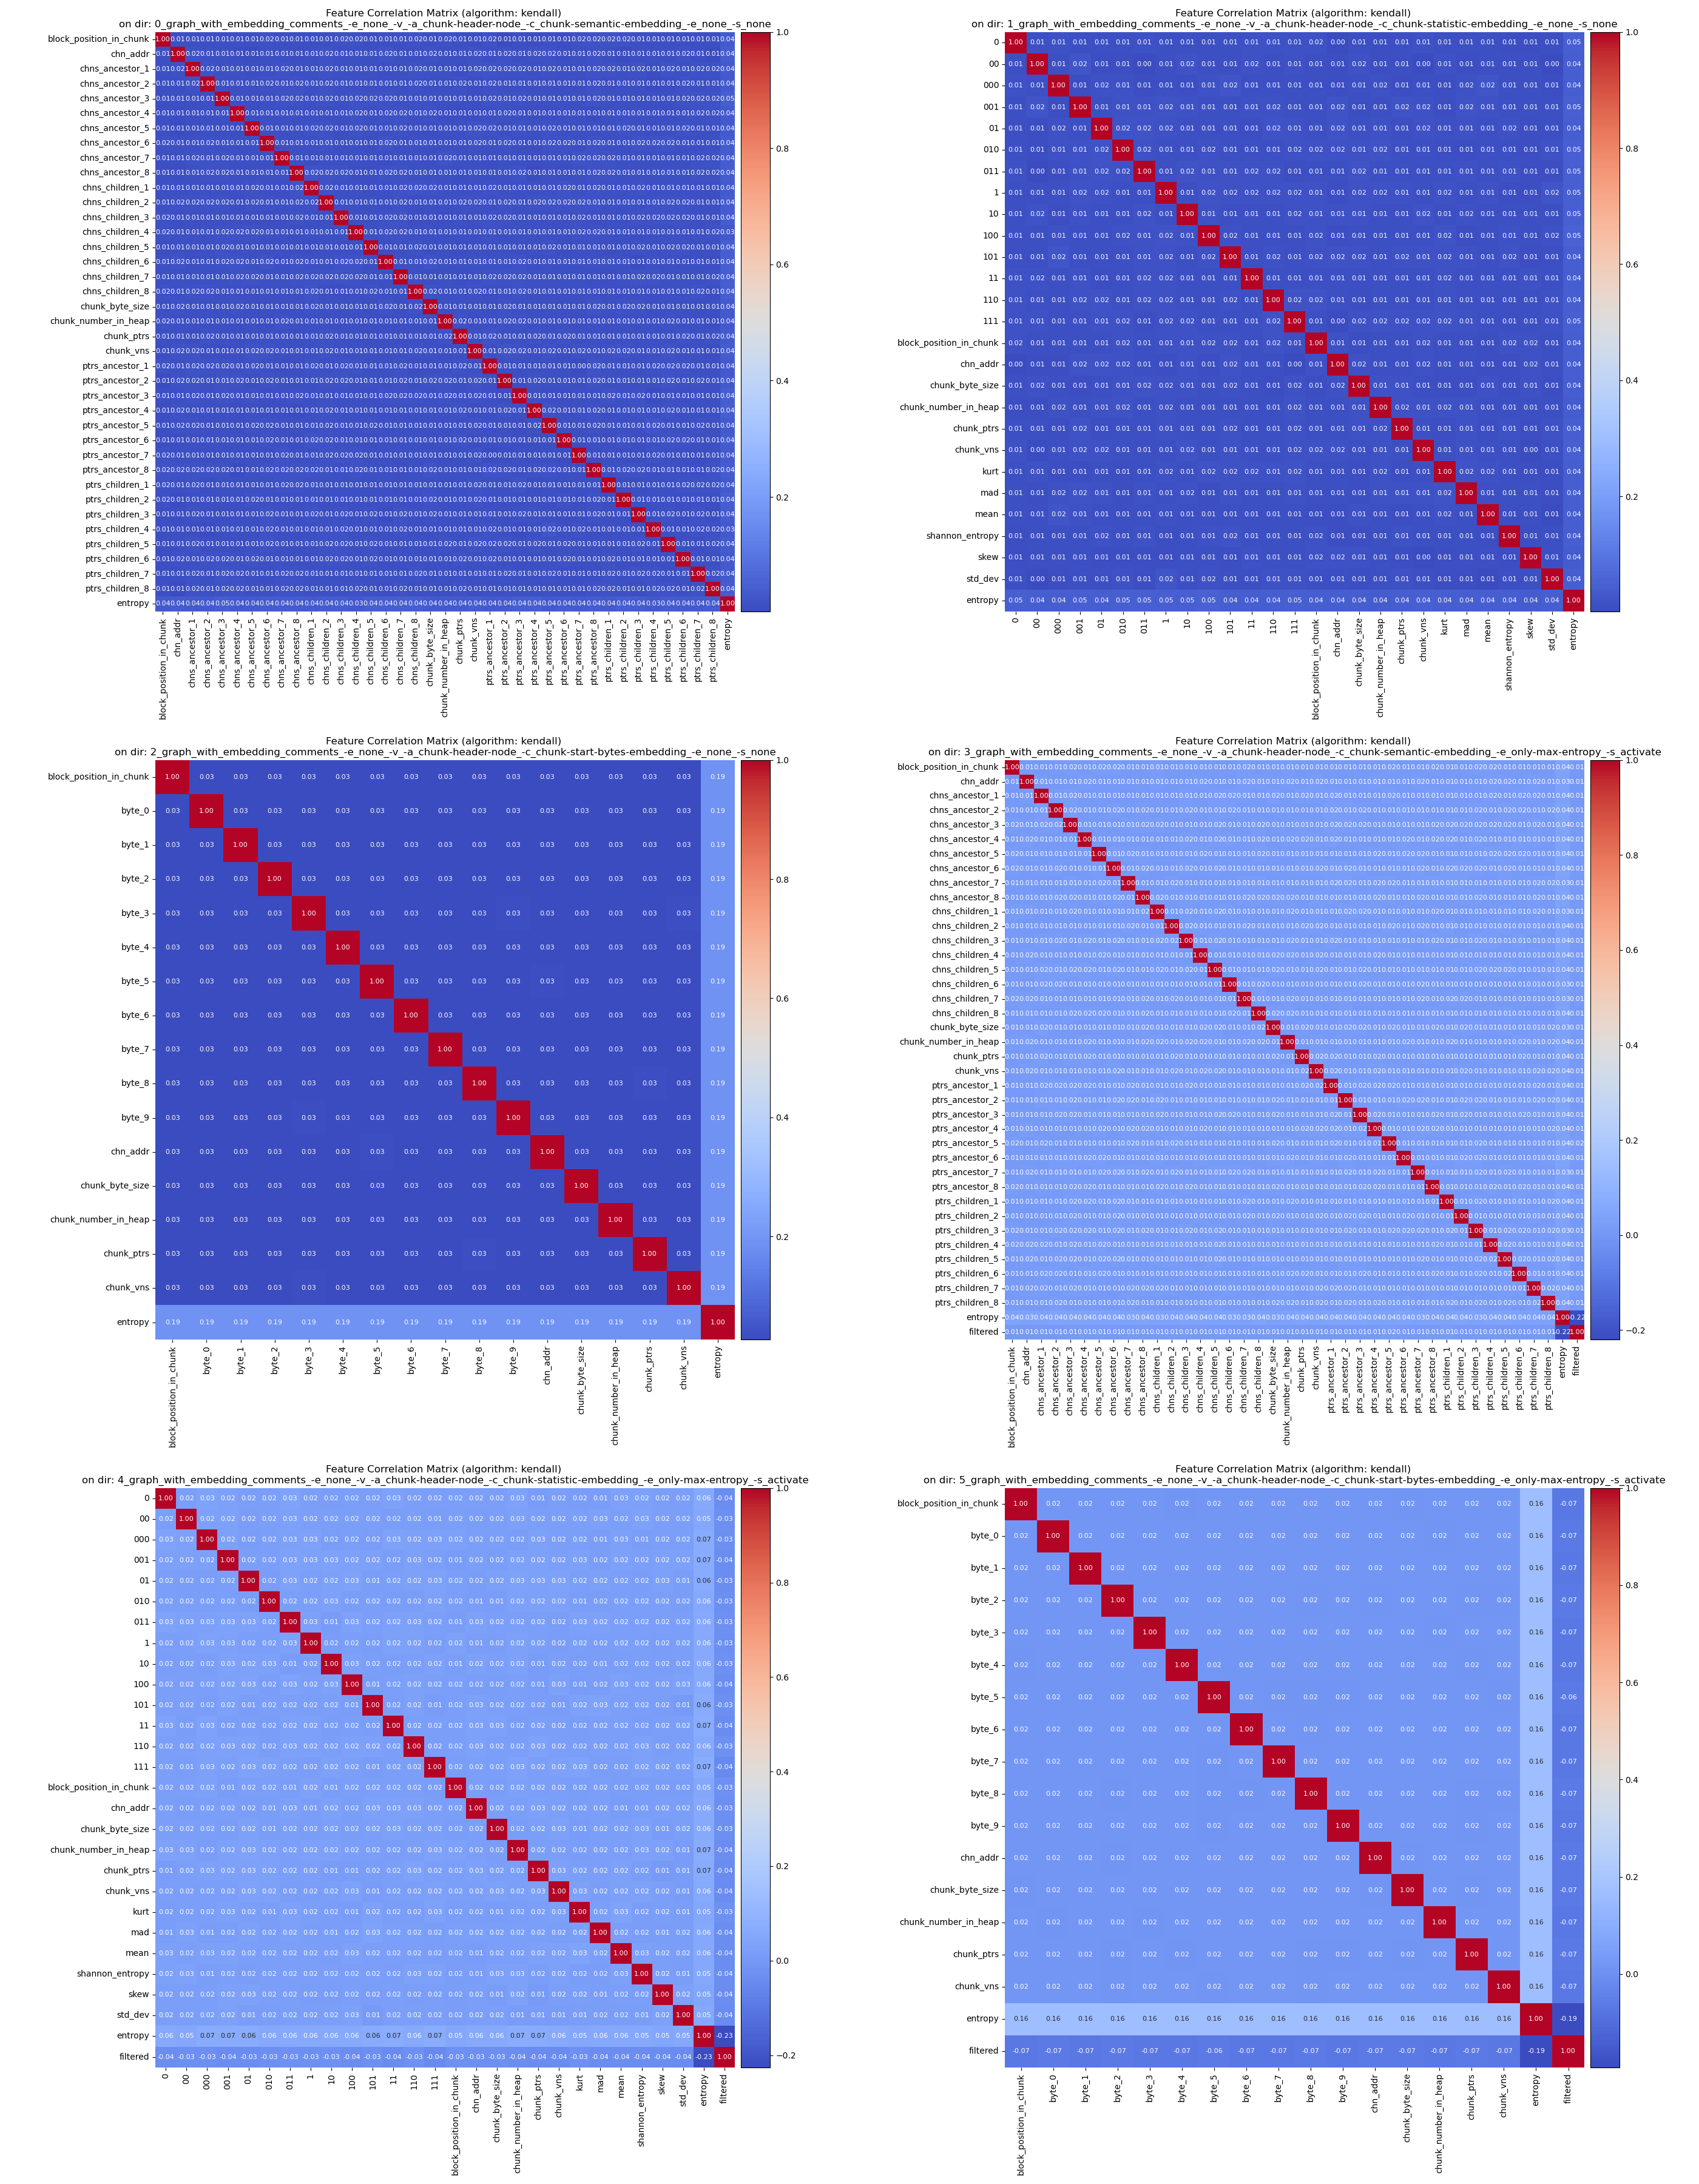
\includegraphics[width=16cm]{feature_engineering/concatenated_1_2023_10_24_kendall.png}
    \caption{Feature correlation matrices on the different Mem2Graph-generated datasets. Used algorithm: Kendall.}
\end{figure}

\begin{figure}[H]\label{results:corr_matrices:pearson}
    \centering
    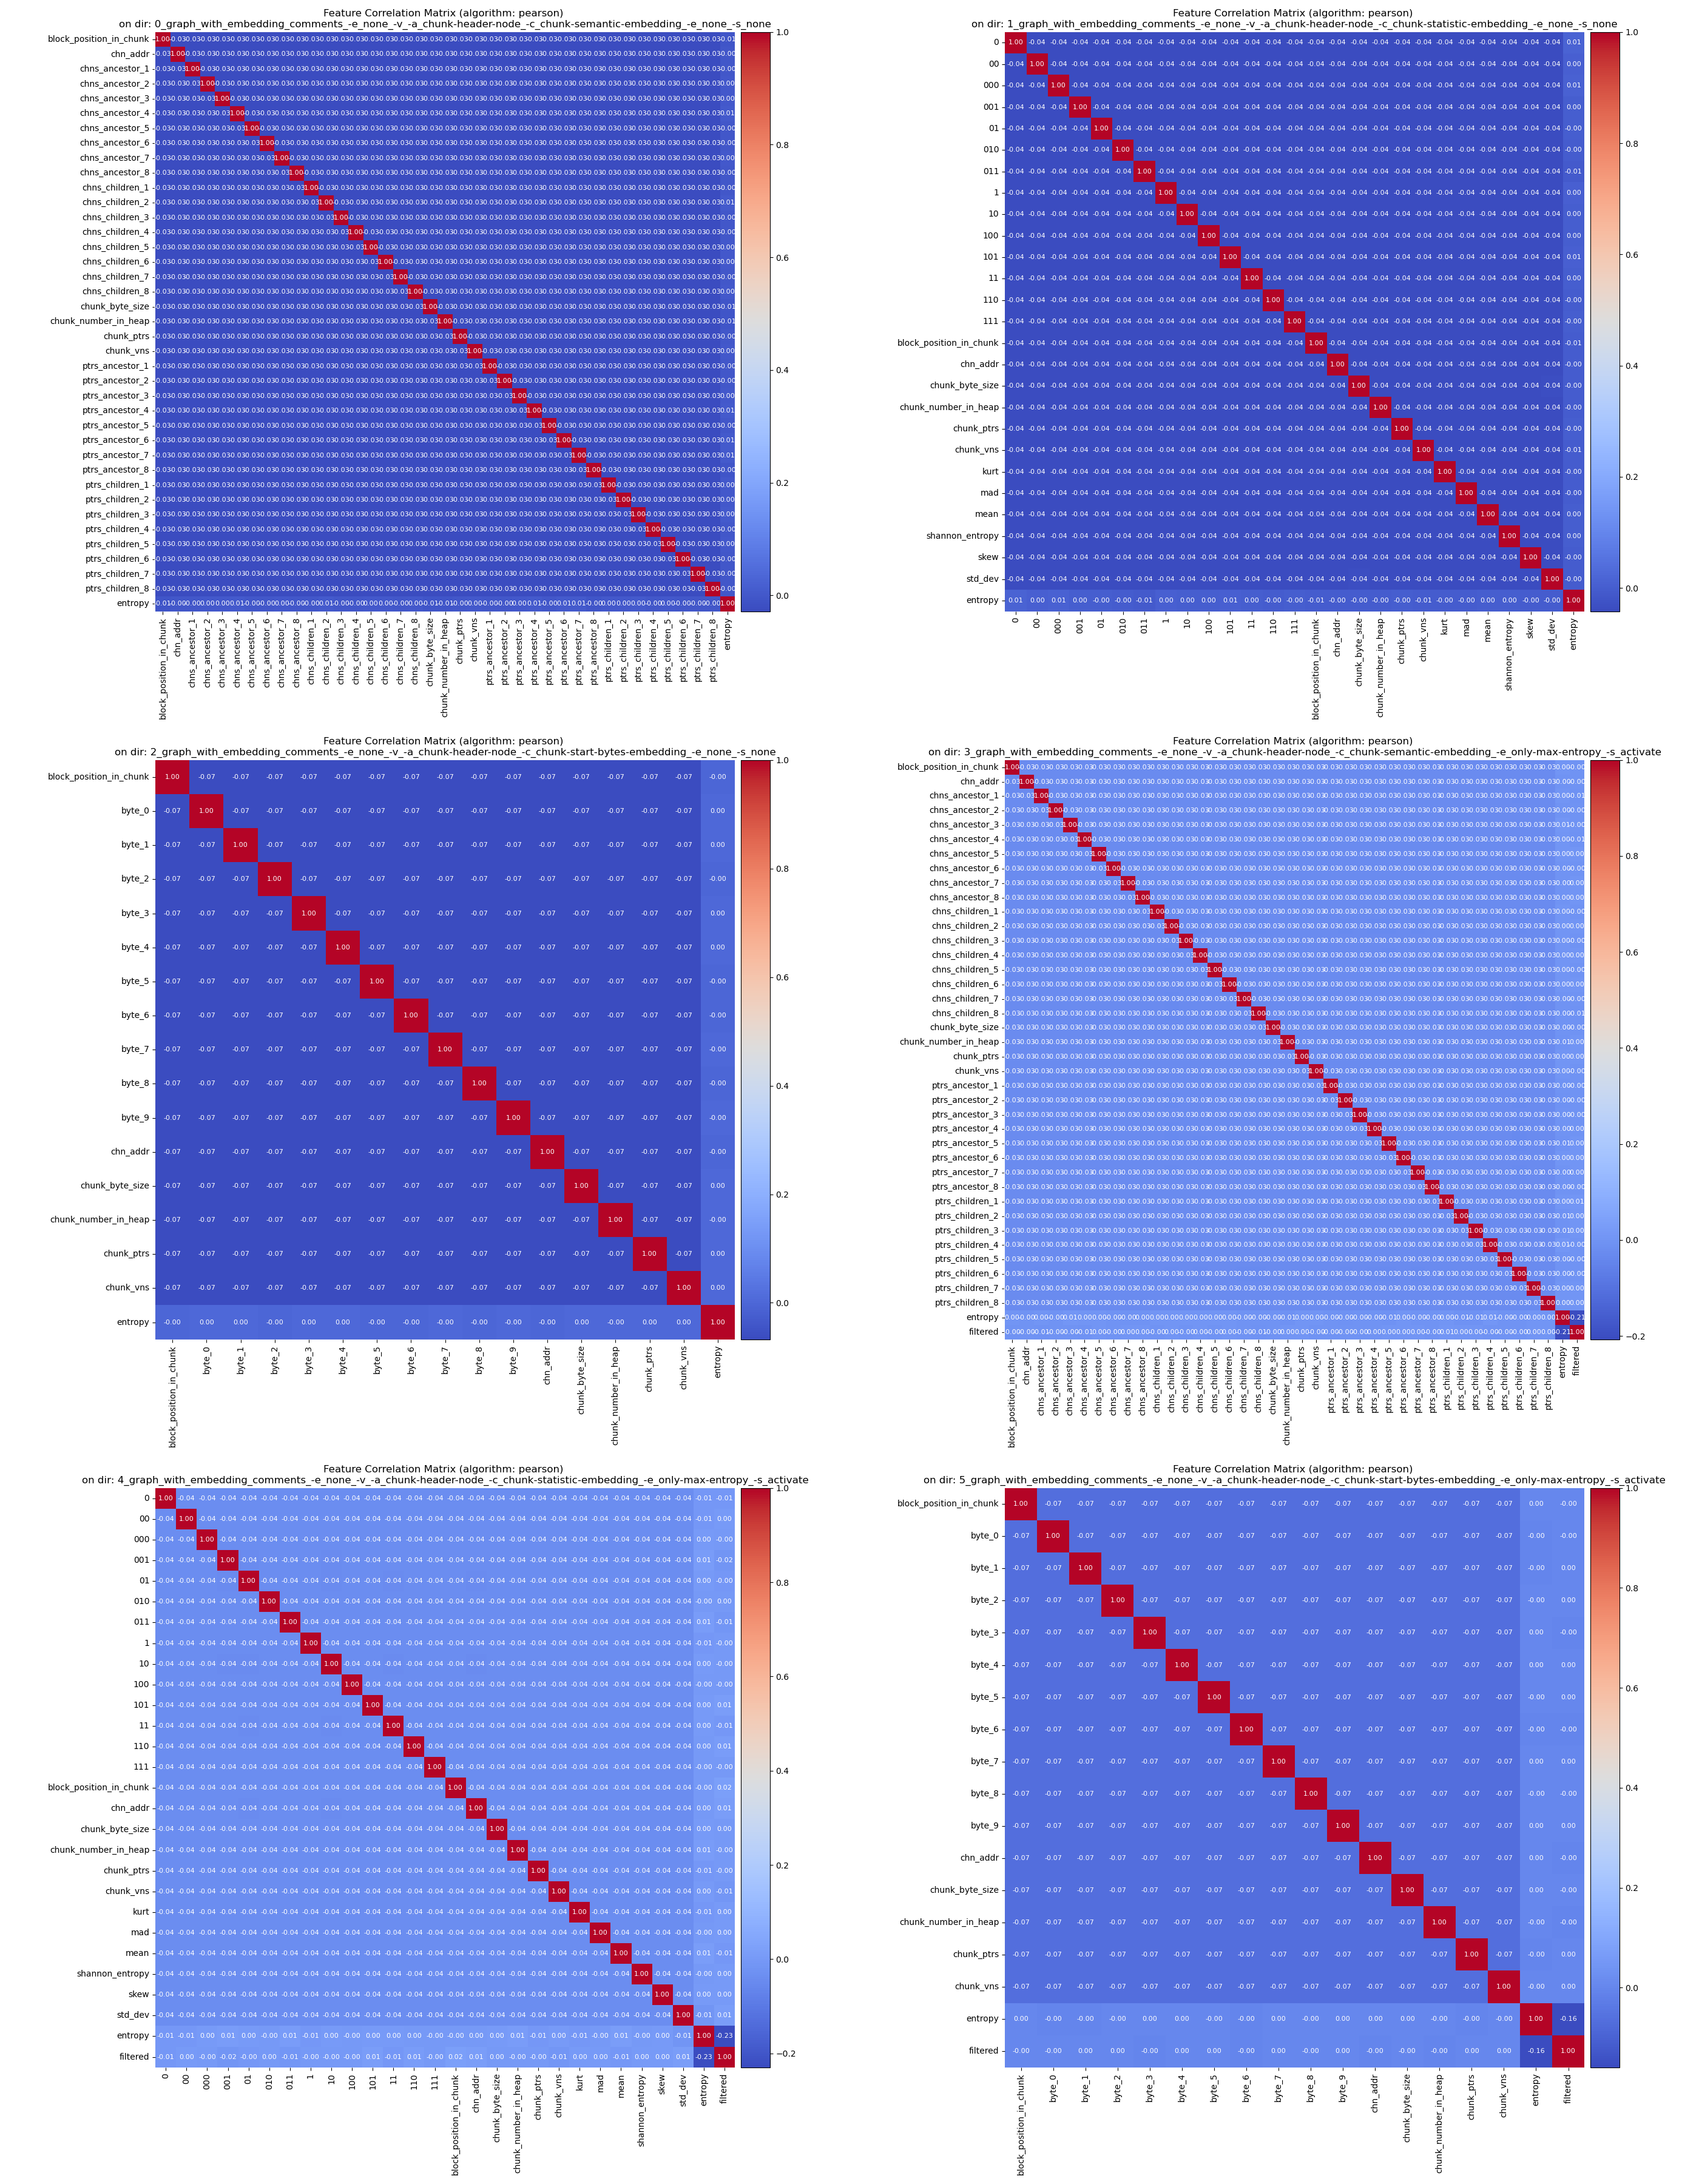
\includegraphics[width=16cm]{feature_engineering/concatenated_2_2023_10_24_pearson.png}
    \caption{Feature correlation matrices on the different Mem2Graph-generated datasets. Used algorithm: Pearson.}
\end{figure}

\begin{figure}[H]\label{results:corr_matrices:spearman}
    \centering
    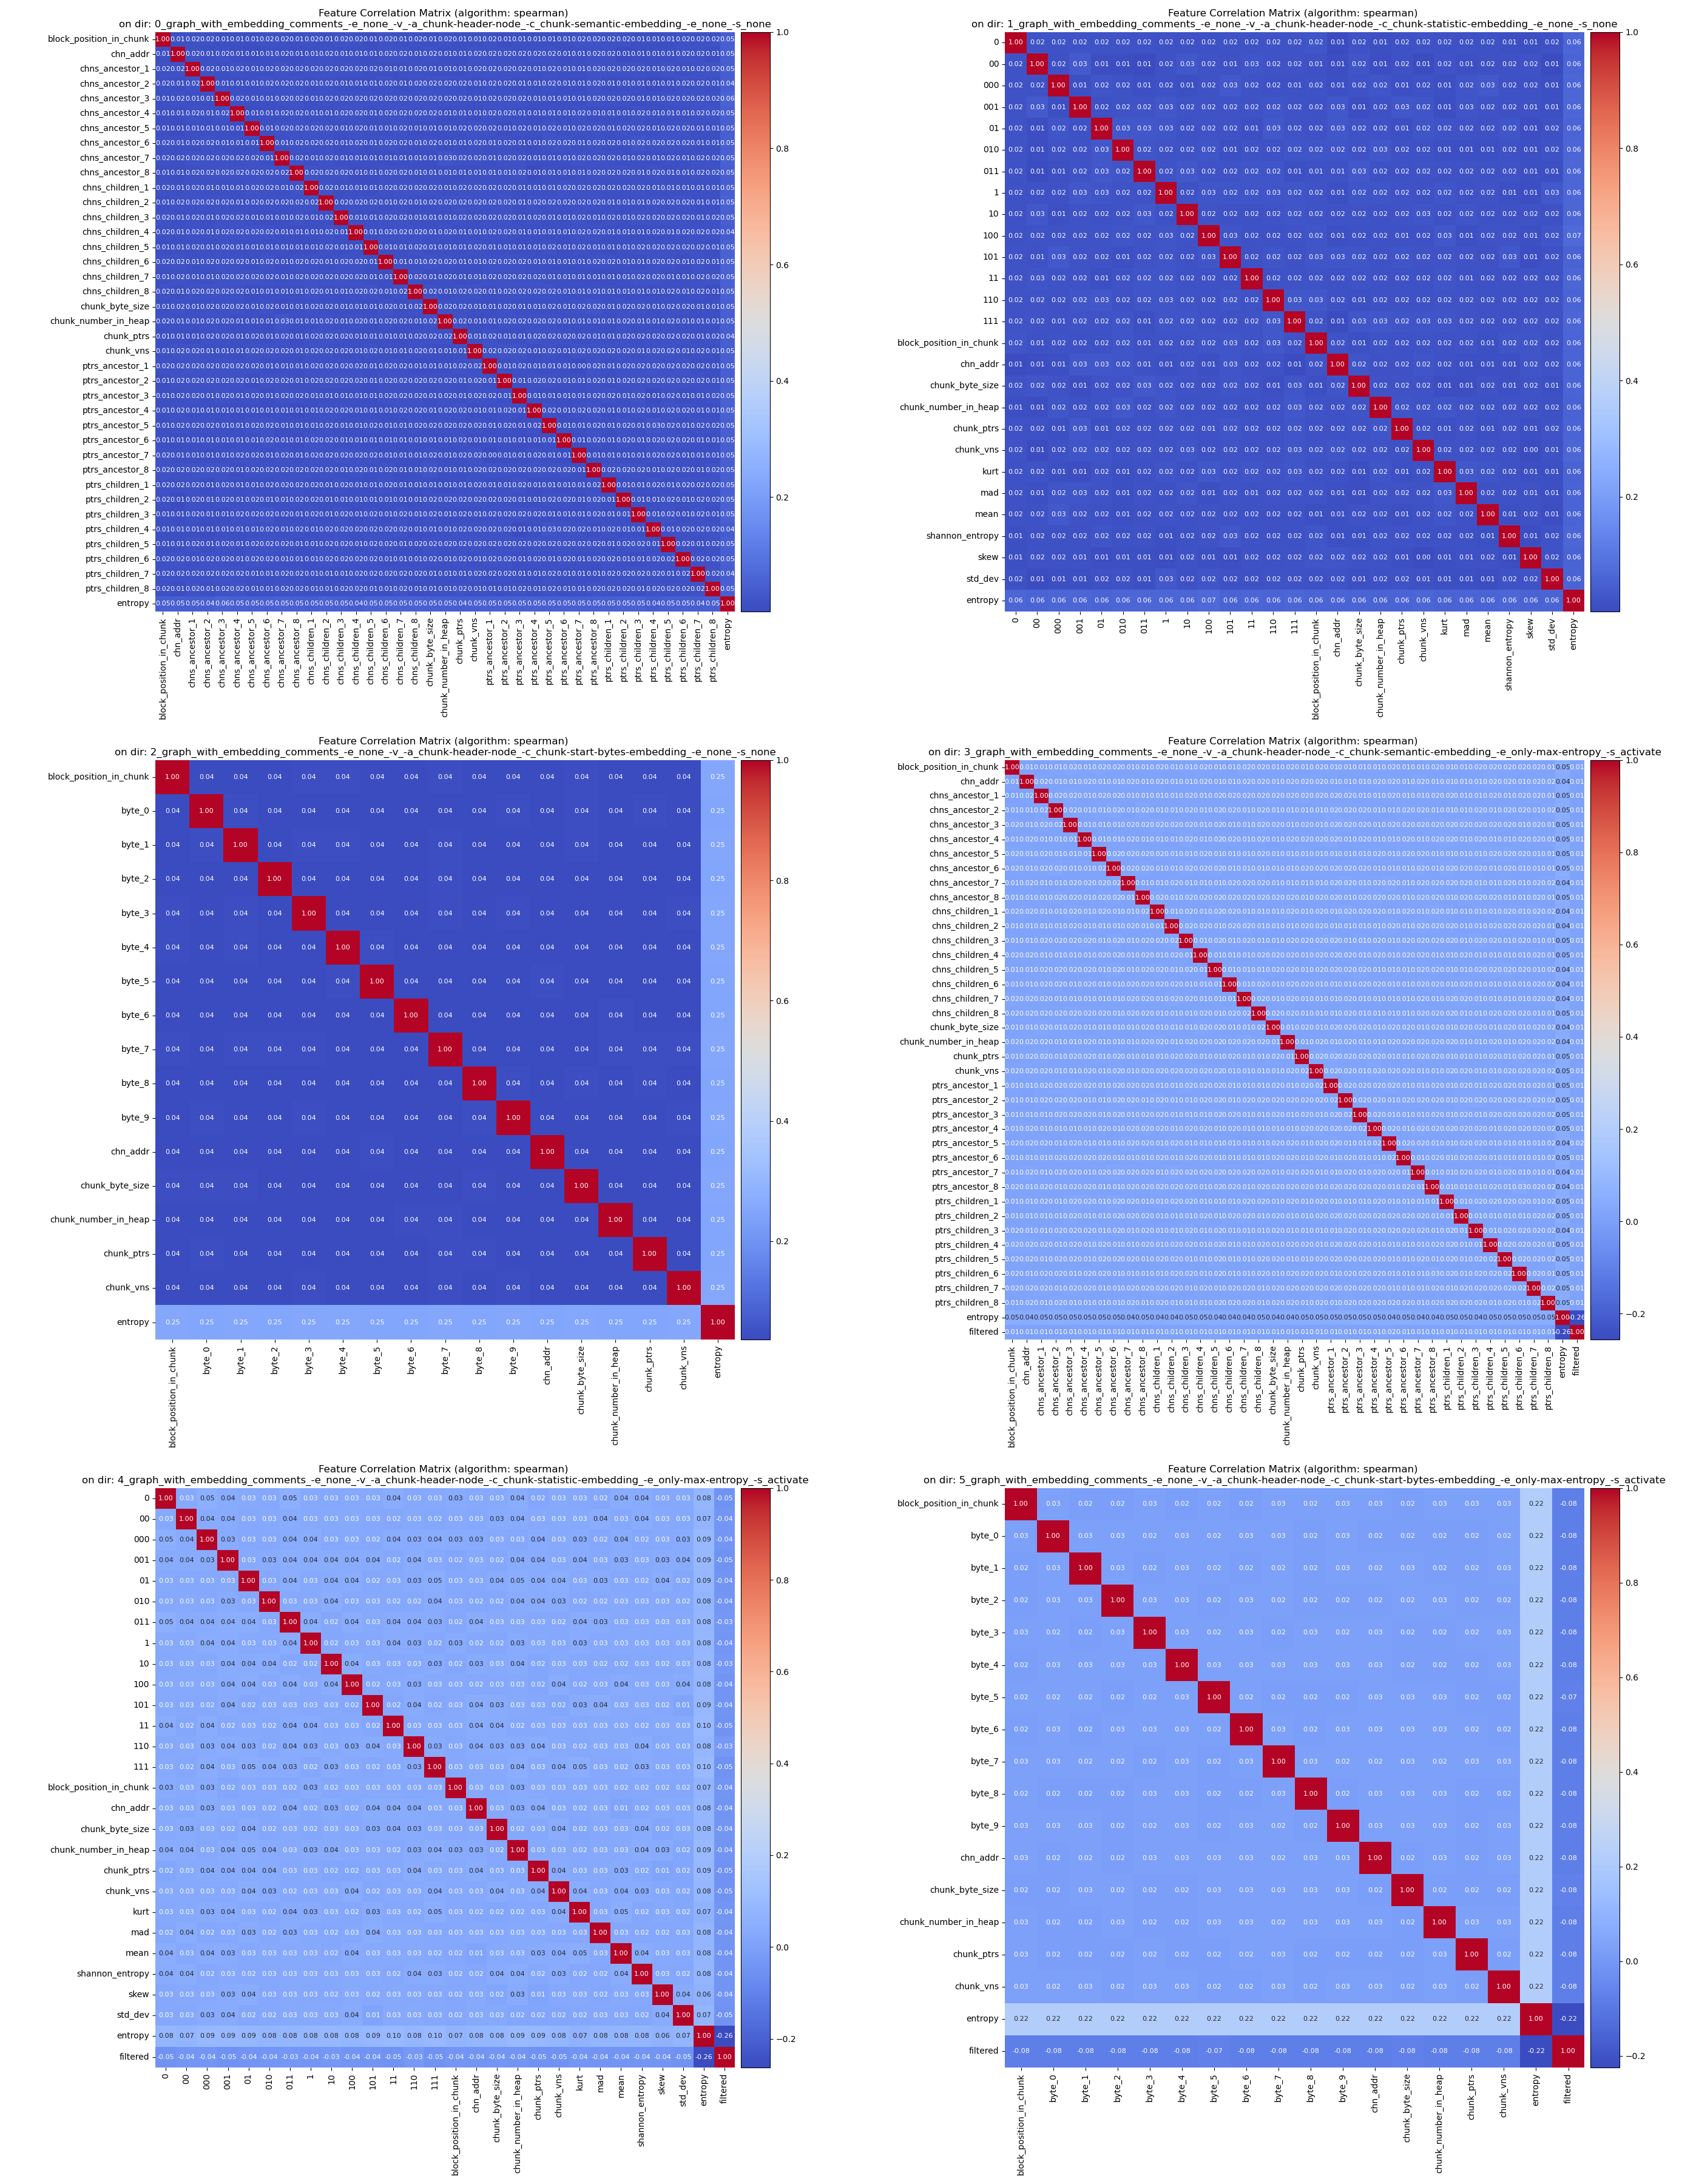
\includegraphics[width=16cm]{feature_engineering/concatenated_3__2023_10_24_spearman.png}
    \caption{Feature correlation matrices on the different Mem2Graph-generated datasets. Used algorithm: Spearman.}
\end{figure}

\section{Classic Model results}


\begin{table}[H]
    \centering
    \caption{Best instances of model: logistic-regression.}
    \begin{tabular}{lcccccc}
      \textbf{Best at}  & \textbf{Precision} & \textbf{Recall} & \textbf{F1 Score} & \textbf{AUC} \\
        precision & 1.0000 & 0.0417 & 0.0800 & 0.5208 \\
        recall & 0.3333 & 0.5000 & 0.4000 & 0.7471 \\
        f1 score & 0.3333 & 0.5000 & 0.4000 & 0.7471 \\
        AUC & 0.2449 & 0.5000 & 0.3288 & 0.7486 \\
    \end{tabular}
\end{table}


\begin{table}[H]
    \centering
    \caption{Best instances of model: random-forest.}
    \begin{tabular}{lcccccc}
      \textbf{Best at}  & \textbf{Precision} & \textbf{Recall} & \textbf{F1 Score} & \textbf{AUC} \\
        precision & 1.0000 & 0.0417 & 0.0800 & 0.5208 \\
        recall & 1.0000 & 0.0833 & 0.1538 & 0.5417 \\
        f1 score & 1.0000 & 0.0833 & 0.1538 & 0.5417 \\
        AUC & 1.0000 & 0.0833 & 0.1538 & 0.5417 \\
    \end{tabular}
\end{table}


\begin{table}[H]
    \centering
    \caption{Best instances of model: sgd-classifier.}
    \begin{tabular}{lcccccc}
      \textbf{Best at}  & \textbf{Precision} & \textbf{Recall} & \textbf{F1 Score} & \textbf{AUC} \\
        precision & 1.0000 & 0.0417 & 0.0800 & 0.5208 \\
        recall & 0.4615 & 1.0000 & 0.6316 & 0.9962 \\
        f1 score & 0.4615 & 1.0000 & 0.6316 & 0.9962 \\
        AUC & 0.4615 & 1.0000 & 0.6316 & 0.9962 \\
    \end{tabular}
\end{table}


\section{Deep Learning GCN Model results}
Best models obtained after the hyperparameter search, on a range of embeddings and models:

\begin{table}[H]
    \centering
    \caption{Best instances of model: very-simple-gcn.}
    \begin{tabular}{lcccccc}
      \textbf{Best at}  & \textbf{Precision} & \textbf{Recall} & \textbf{F1 Score} & \textbf{AUC} \\
        precision & 0.6000 & 0.5000 & 0.5455 & 0.7489 \\
        recall & 0.2609 & 1.0000 & 0.4138 & 0.9907 \\
        f1 score & 0.6000 & 0.5000 & 0.5455 & 0.7489 \\
        AUC & 0.2609 & 1.0000 & 0.4138 & 0.9907 \\
    \end{tabular}
\end{table}

\begin{table}[H]
    \centering
    \caption{Best instances of model: simple-gcn.}
    \begin{tabular}{lcccccc}
      \textbf{Best at}  & \textbf{Precision} & \textbf{Recall} & \textbf{F1 Score} & \textbf{AUC} \\
        precision & 0.5000 & 0.5000 & 0.5000 & 0.7484 \\
        recall & 0.2308 & 1.0000 & 0.3750 & 0.9891 \\
        f1 score & 0.5000 & 0.5000 & 0.5000 & 0.7484 \\
        AUC & 0.2609 & 1.0000 & 0.4138 & 0.9907 \\
    \end{tabular}
\end{table}

\begin{table}[H]
    \centering
    \caption{Best instances of model: first-gcn.}
    \begin{tabular}{lcccccc}
      \textbf{Best at}  & \textbf{Precision} & \textbf{Recall} & \textbf{F1 Score} & \textbf{AUC} \\
        precision & 0.5000 & 0.5000 & 0.5000 & 0.7484 \\
        recall & 0.2727 & 1.0000 & 0.4286 & 0.9913 \\
        f1 score & 0.5000 & 0.5000 & 0.5000 & 0.7484 \\
        AUC & 0.2727 & 1.0000 & 0.4286 & 0.9913 \\
    \end{tabular}
\end{table}

\begin{table}[H]
    \centering
    \caption{Best instances of model: gcn-with-dropout.}
    \begin{tabular}{lcccccc}
      \textbf{Best at}  & \textbf{Precision} & \textbf{Recall} & \textbf{F1 Score} & \textbf{AUC} \\
        precision & 0.3500 & 0.2333 & 0.2800 & 0.6152 \\
        recall & 0.0863 & 0.8000 & 0.1558 & 0.8810 \\
        f1 score & 0.2110 & 0.7667 & 0.3309 & 0.8767 \\
        AUC & 0.0863 & 0.8000 & 0.1558 & 0.8810 \\
    \end{tabular}
\end{table}

\begin{table}[H]
    \centering
    \caption{Best instances of model: advanced-gcn.}
    \begin{tabular}{lcccccc}
      \textbf{Best at}  & \textbf{Precision} & \textbf{Recall} & \textbf{F1 Score} & \textbf{AUC} \\
        precision & 0.2097 & 0.4333 & 0.2826 & 0.7129 \\
        recall & 0.0533 & 0.9000 & 0.1006 & 0.8943 \\
        f1 score & 0.2097 & 0.4333 & 0.2826 & 0.7129 \\
        AUC & 0.1552 & 0.9000 & 0.2647 & 0.9390 \\
    \end{tabular}
\end{table}

\section{Compared Performances of models and embeddings}
* Comparing all computed results, on a maximum number of input graph of 16, which is really low. This is due to the fact that we have so many hyperparameters, embeddings and models to compare.
* Results on 7976 machine learning pipelines, for a cumulated compute time of over 100h.

\begin{table}[H]
    \centering
    \caption{Results for the model very-simple-gcn}
    \begin{tabular}{lcccccc}
      \textbf{Model}  & \textbf{Best Precision} & \textbf{Best Recall} & \textbf{Best F1 Score} & \textbf{Best AUC} \\
        advanced-gcn & 0.2097 & 0.9000 & 0.2826 & 0.9390 \\
        first-gcn & 0.5000 & 1.0000 & 0.5000 & 0.9913 \\
        gcn-with-dropout & 0.3500 & 0.8000 & 0.3309 & 0.8810 \\
        logistic-regression & 1.0000 & 0.5000 & 0.4000 & 0.7486 \\
        random-forest & 1.0000 & 0.0833 & 0.1538 & 0.5417 \\
        sgd-classifier & 1.0000 & 1.0000 & 0.6316 & 0.9962 \\
        simple-gcn & 0.5000 & 1.0000 & 0.5000 & 0.9907 \\
        very-simple-gcn & 0.6000 & 1.0000 & 0.5455 & 0.9907 \\
    \end{tabular}
\end{table}

\begin{figure}[H]\label{results:compare:models:full}
    \centering
    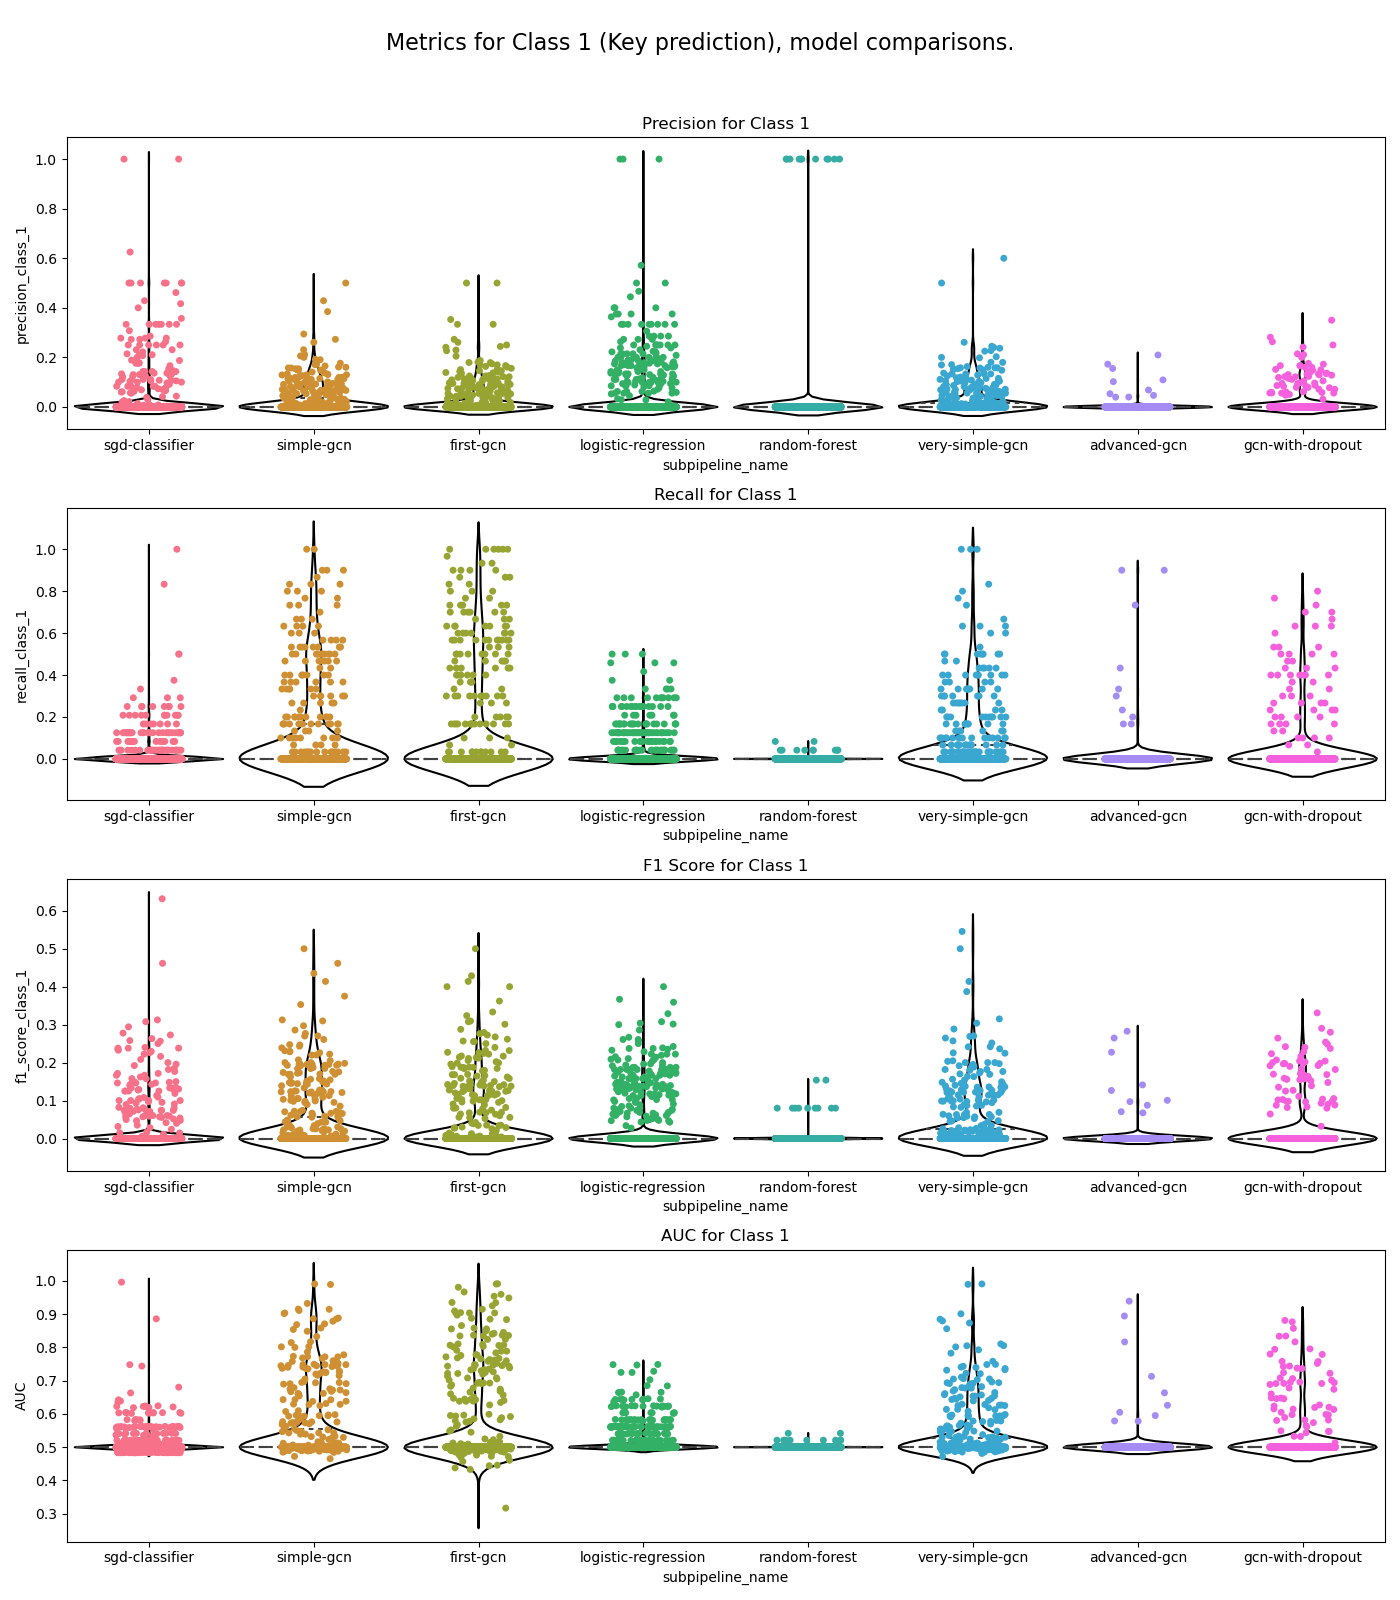
\includegraphics[width=16cm]{plots/models_comparison_metrics.png}
    \caption{Visualization of the result metrics use to compare model performance on memory graphs, for different embeddings and hyperparameters.}
\end{figure}

\begin{figure}[H]\label{results:compare:embeddings:full}
    \centering
    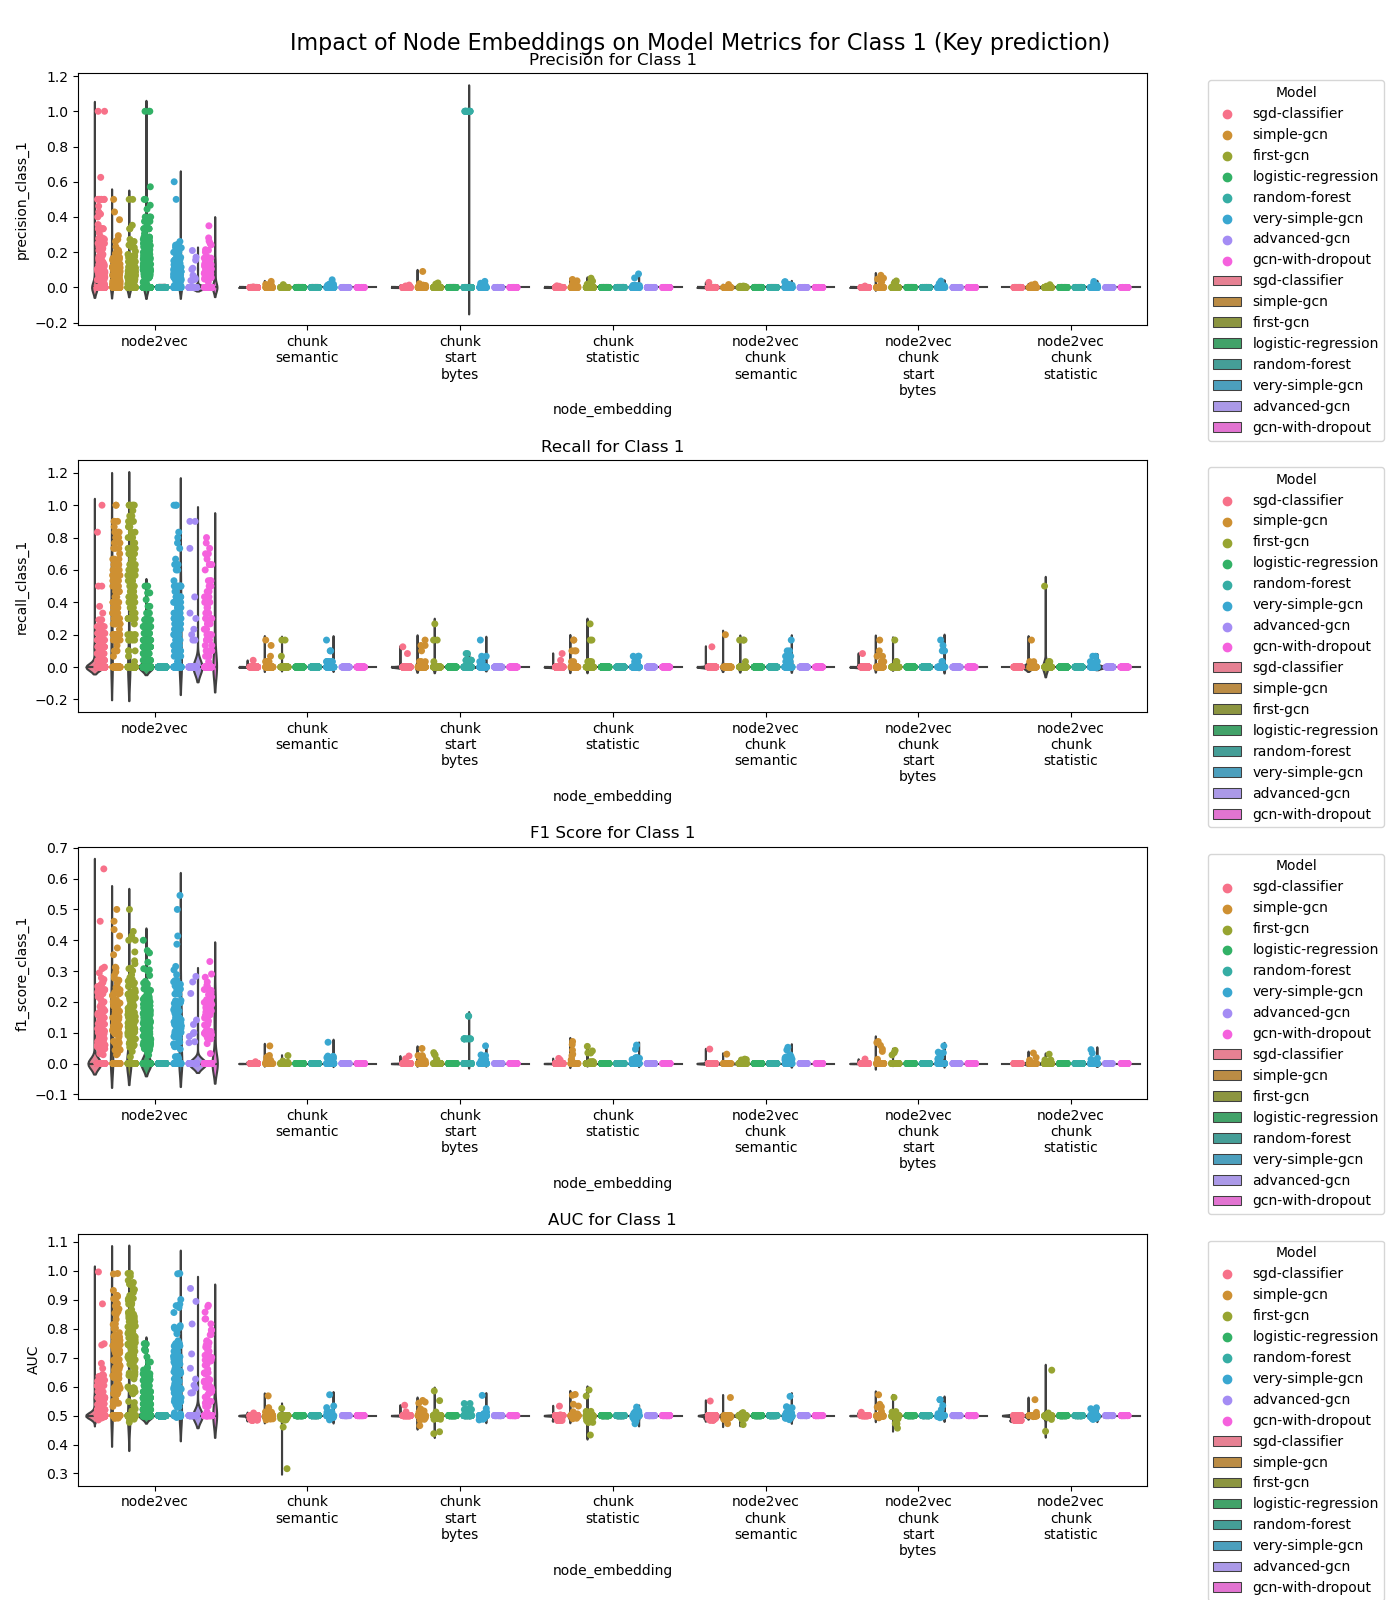
\includegraphics[width=16cm]{plots/embedding_comparison_metrics.png}
    \caption{Visualization of the result metrics use to compare model performance per memory graph node embedding strategies.}
\end{figure}



\chapter{Discussion}\label{chap:discussion}

Discuss the results. What is the outcome of your experiments?
\chapter{Conclusion}\label{chap:conclusion}

% Summarize the thesis and provide a outlook on future work.

The evolving landscape of cybersecurity necessitates robust techniques for safeguarding digital communications. OpenSSH, a pivotal element in this landscape, is a popular implementation of the Secure Shell (\acrshort{ssh}) protocol, which enables secure communication between two networked devices. The protocol is widely used in the industry, particularly in the context of remote access to servers. Using digital forensic techniques, it is possible to extract the SSH keys from memory dumps, which can then be used to decode encrypted communications thus allowing the monitoring of controlled systems. At the crux of this Masterarbeit is the development of algorithms and machine learning models to predict SSH keys within these heap dumps, focusing on using graph-like-structures and vectorization for custom embeddings. With an interdisciplinary approach that fuses traditional feature engineering with graph-based methods as well as memory modelization for inductive reasoning and learning inspired by recent developments in \acrfull{kg}s, this research not only leverages existing machine learning paradigms but also explores new avenues, such as \acrfull{gcn} applied to memory forensics. The present work also introduces a new memory forensics tool, \textit{mem2graph}, which is designed to be modular and extensible, and which can be used to generate memory graphs from memory dumps. 

\section{Summary of Results}
Below is a summary of the results achieved in the present work.

\subsection{Memory Graph Generation}
This masterarbeit has introduced a range of algorithms able to generate memory graphs from memory dumps. The algorithms are designed to be as generic as possible, and can be applied to any memory dump dataset. The algorithms are mostly implemented in the \textit{mem2graph} program.

With those algorithm, it is possble to parse a RAW heap dump file, and transform it into a memory graph. The memory graph is a graph-like structure, where each node represents a memory block with a precise address in the heap. Each edge represents either a pointer pointing to another block, or materialize the fact that a block belongs to a specific chunk. 

The memory graph can be used to extract features from the memory dump, and to apply machine learning algorithms to the memory dump. It can also be used for direct graph visualization.

\subsection{Feature Engineering and Embeddings}

\subsection{Classic Machine Learning Models}

\subsection{Deep Learning GCN Models}


\section{Outlook on Future Work}\label{conclusion:sec:future_work}

% What are the next steps? What are the open questions? What are the limitations of your work?

The current report, in conjunction with the associated Masterarbeit, has introduced numerous novel algorithms and implementations. These have been instrumental in addressing the initial research questions. However, as with most research endeavors, new queries and potential avenues for enhancement have emerged, paving the way towards further exploration.

The methodologies and algorithms introduced for the OpenSSH memory dump dataset are versatile and can be extended to other memory dump datasets utilizing the GLIBC library. Given that this library is the default for Linux, adapting the methods from this Masterarbeit to other applications requires minimal effort. The \textit{mem2graph} program is inherently modular and built for extensibility. Furthermore, this tool can be employed to produce memory graphs for diverse datasets. Thanks to the universal character of the generated embeddings and memory graphs, new datasets can be readily integrated into the \acrshort{ml} and \acrshort{dl} pipelines crafted in Python. While an extensive array of features and embedding techniques have been explored in this report, there remains ample opportunity for innovative experimentation.

For a seamless fusion of machine learning into the \textit{mem2graph} program, further effort is required. Embedding machine learning immediately post-memory graph creation can substantially boost efficiency, particularly when aiming to craft a real-time OpenSSH memory forensics utility. However, this integration is challenging due to the current limited \acrshort{ml} support within Rust.

Another avenue for enhancement involves analyzing the effects of different C libraries on allocated chunks and the layout of heap dump memory. Investigating various languages could also be insightful. Depending on the level of variation encountered, modifications to the algorithms might be required, especially concerning the architecture involved in generating or extracting heap dump configurations. Pursuing this direction could significantly advance the development of a universal machine learning-assisted memory forensics tool for key extraction.

While the background section underscores the vast array of \acrshort{ml} architectures available, it's clear that not all can be thoroughly explored. This research has primarily addressed the most common and promising ones, yet numerous others await investigation. The tools crafted to bolster \acrshort{ml} pipelines present a solid foundation for such endeavors. Another dimension to consider is hyperparameter optimization. Given the constraints of time and resources, only certain parameter ranges were tested. Expanding these tests, incorporating larger datasets, and harnessing increased computational capacity can directly enhance performance.




%%%%%%%%%%%%%%%%%%%%%%%%%%%%%%%%%%%%%%%%%%%%%%%%%%%%%%%%%%%%%%%%%%%%%%%%%%%%%%%%%%%%%%%%%
\newpage
% -- Appendix (optional)
\begin{appendices}
    % !TeX spellcheck = en_US
% !TeX encoding = UTF-8
\chapter*{Appendix}

\section{Code and files}

\begin{lstlisting}[style=text, caption={The DOT file of uncompressed block memgraph, here \textit{Training/basic/V\_7\_1\_P1/24/17016-1643962152-heap.raw}, with real addresses. Output is cropped.}, label={appendix:dot:17016-1643962152:cropped}]
    strict digraph "17016-1643962152" {
        "CHN(0x558343d21d40)" [label="CHN(1)" color="cyan" style=filled shape=square];
        "CHN(0x558343d1a448)" [label="CHN(2)" color="cyan" style=filled shape=square];
        "VN(0x558343d1a450)" [label="VN" color="grey" style=filled];
        "VN(0x558343d1a458)" [label="VN" color="grey" style=filled];
        "PN(0x558343d24ae8)" [label="PN" color="orange" style=filled shape=hexagon];
        "KN_KEY_A(0x558343d29460)" [label="KN(A)" color="green" style=filled];
        "KN_KEY_B(0x558343d2b960)" [label="KN(B)" color="green" style=filled];
        "CHN(0x558343d21d40)" -> "KN_KEY_A(0x558343d29460)" [label="dts" weight=1]
        "PN(0x558343d204e8)" -> "KN_KEY_A(0x558343d29460)" [label="ptr" weight=1]
        "CHN(0x558343d21d40)" -> "KN_KEY_B(0x558343d2b960)" [label="dts" weight=1]
        "PN(0x558343d2deb8)" -> "KN_KEY_B(0x558343d2b960)" [label="ptr" weight=1]
        "CHN(0x558343d21d40)" -> "KN_KEY_C(0x558343d29080)" [label="dts" weight=1]
        "PN(0x558343d204e0)" -> "KN_KEY_C(0x558343d29080)" [label="ptr" weight=1]
        "PN(0x558343d24ae8)" -> "VN(0x558343d1a010)" [label="ptr" weight=1]
        "PN(0x558343d1a240)" -> "VN(0x558343d20680)" [label="ptr" weight=1]
    }
\end{lstlisting}

\section{Memory Graphs}

\begin{figure}[H]\label{appendix:mem_graph:302-1644391327:full}
    \centering
    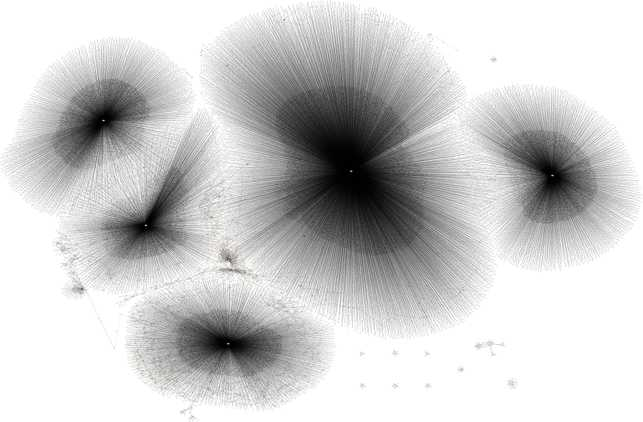
\includegraphics[width=16cm]{graphs/test_graph_from_302-1644391327_vn-sfdp.jpg}
    \caption{Visualization of the full memory graph generated from \textit{Training/scp/V\_7\_8\_P1/16/302-1644391327-heap.raw}.}
\end{figure}

\begin{figure}[H]\label{appendix:mem_graph:17016-1643962152:full}
    \centering
    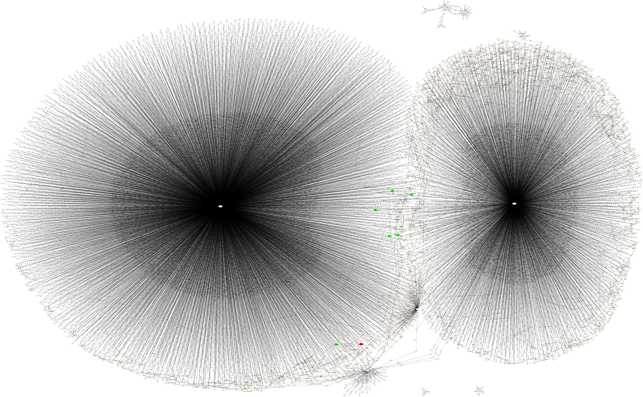
\includegraphics[width=16cm]{graphs/Training_basic_V_7_1_P1_24_17016-1643962152-heap.raw_dot_vn-sfdp.jpg}
    \caption{Visualization of the full memory graph generated from \textit{Training/basic/V\_7\_1\_P1/24/17016-1643962152-heap.raw}.}
\end{figure}

\begin{figure}[H]\label{appendix:mem_graph:17016-1643962152:truncated}
    \centering
    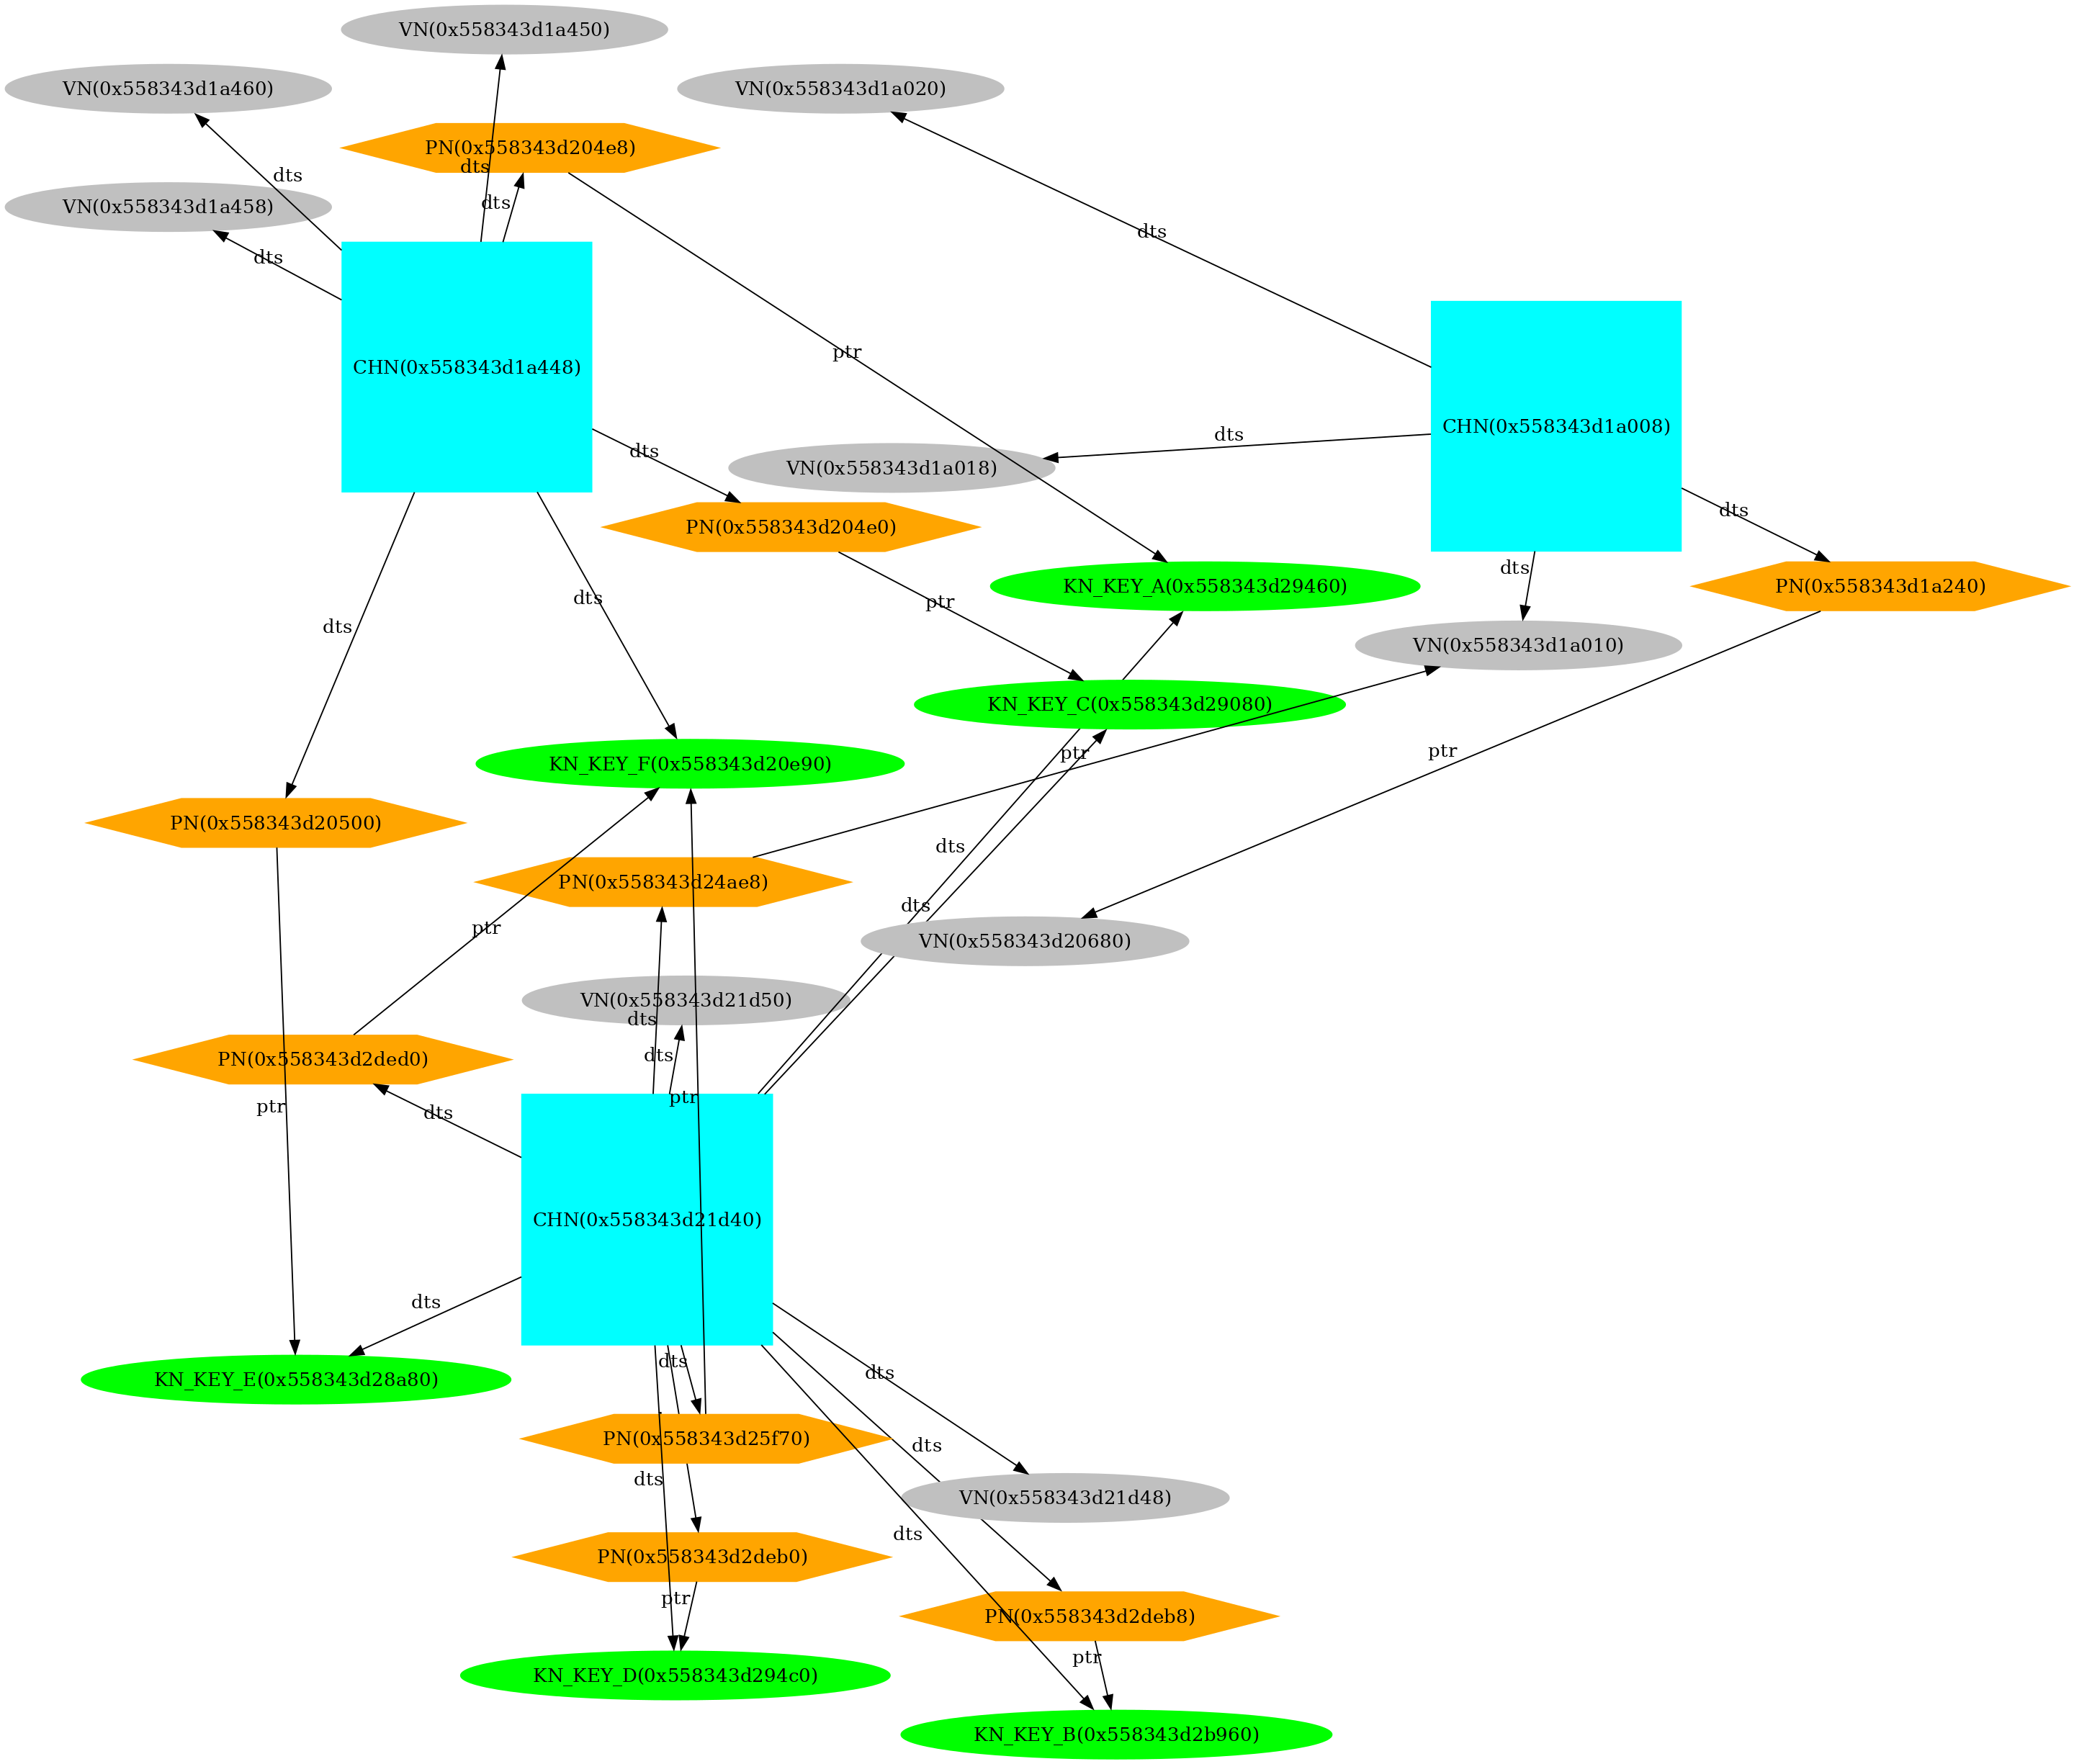
\includegraphics[width=16cm]{graphs/17016-1643962152_truncated.png}
    \caption{Visualization of a truncated memory graph generated from \textit{Training/basic/V\_7\_1\_P1/24/17016-1643962152-heap.raw}. Here with real addresses.}
\end{figure}

Generated using a slightly different command, for better layout of the nodes:

\begin{lstlisting}[language=bash, caption={Command used to generate the memory graph visualization of \textit{Training/basic/V\_7\_1\_P1/24/17016-1643962152-heap.raw} here using real addresses.}]
    sfdp -Gsize=30! -Goverlap=ortho -Tpng 17016-1643962152_truncated.gv > 17016-1643962152_truncated.png
\end{lstlisting}

\begin{figure}[H]
    \centering
    \includegraphics[width=16cm]{graphs/chunk_top_vn_semantic_home_onyr_code_phdtrack_phdtrack_data_clean_8708-1643979488-heap.raw_dot_no_vn_chn_annotation_no_vn-sfdp.png}
    \caption{Visualization of a chunk memory graph generated from \textit{Validation/Validation/basic/V\_7\_8\_P1/24/8708-1643979488-heap.raw}.}
\end{figure}

\begin{figure}[H]
    \centering
    \includegraphics[width=16cm]{graphs/chunk_top_vn_semantic_home_onyr_code_phdtrack_phdtrack_data_clean_28621-1643890740-heap.raw_dot_no_vn_chn_annotation_no_vn-sfdp.png}
    \caption{Visualization of a chunk memory graph generated from \textit{Training/Training/basic/V\_6\_8\_P1/24/28621-1643890740-heap.raw}.}
\end{figure}

\section{Latest ML Experiment results}
The following are the latest results for ML experiments. Those tables were generated after the submission of the thesis.

\begin{table}[H]
    \centering
    \caption{Best instance for each model, with respect to accuracy.}
    \begin{tabular}{|l|c|c|c|c|c|c|} \hline 
      \textbf{Model}  & \textbf{Accuracy} & \textbf{Precision} & \textbf{Recall} & \textbf{F1 Score} & \textbf{Embedding}  \\ \hline 
        random-forest & 0.9984 & 1.0000 & 0.0833 & 0.1538 & chunk-start-bytes \\ \hline 
        sgd-classifier & 0.9984 & 0.6250 & 0.2083 & 0.3125 & node2vec \\ \hline 
        logistic-regression & 0.9983 & 1.0000 & 0.0417 & 0.0800 & node2vec \\ \hline 
        advanced-gcn & 0.9969 & 0.0000 & 0.0000 & 0.0000 & node2vec \\ \hline 
        gcn-with-dropout & 0.9969 & 0.0000 & 0.0000 & 0.0000 & node2vec \\ \hline 
        first-gcn & 0.9963 & 0.0000 & 0.0000 & 0.0000 & node2vec-chunk-statistic \\ \hline 
        simple-gcn & 0.9962 & 0.0000 & 0.0000 & 0.0000 & chunk-statistic \\ \hline 
        very-simple-gcn & 0.9959 & 0.0000 & 0.0000 & 0.0000 & node2vec \\ \hline 
    \end{tabular}
\end{table}


\begin{table}[H]
    \centering
    \caption{Best instance for each model, with respect to precision.}
    \begin{tabular}{|l|c|c|c|c|c|c|} \hline 
      \textbf{Model}  & \textbf{Accuracy} & \textbf{Precision} & \textbf{Recall} & \textbf{F1 Score} & \textbf{Embedding}  \\ \hline 
        logistic-regression & 0.9944 & 1.0000 & 0.0417 & 0.0800 & node2vec \\ \hline 
        random-forest & 0.9983 & 1.0000 & 0.0417 & 0.0800 & chunk-start-bytes \\ \hline 
        sgd-classifier & 0.9983 & 1.0000 & 0.0417 & 0.0800 & node2vec \\ \hline 
        very-simple-gcn & 0.9946 & 0.6000 & 0.5000 & 0.5455 & node2vec \\ \hline 
        first-gcn & 0.9935 & 0.5000 & 0.5000 & 0.5000 & node2vec \\ \hline 
        simple-gcn & 0.9935 & 0.5000 & 0.5000 & 0.5000 & node2vec \\ \hline 
        gcn-with-dropout & 0.9920 & 0.3500 & 0.2333 & 0.2800 & node2vec \\ \hline 
        advanced-gcn & 0.9898 & 0.2097 & 0.4333 & 0.2826 & node2vec \\ \hline 
    \end{tabular}
\end{table}


\begin{table}[H]
    \centering
    \caption{Best instance for each model, with respect to recall.}
    \begin{tabular}{|l|c|c|c|c|c|c|} \hline 
      \textbf{Model}  & \textbf{Accuracy} & \textbf{Precision} & \textbf{Recall} & \textbf{F1 Score} & \textbf{Embedding}  \\ \hline 
        first-gcn & 0.9826 & 0.2727 & 1.0000 & 0.4286 & node2vec \\ \hline 
        sgd-classifier & 0.9924 & 0.4615 & 1.0000 & 0.6316 & node2vec \\ \hline 
        simple-gcn & 0.9783 & 0.2308 & 1.0000 & 0.3750 & node2vec \\ \hline 
        very-simple-gcn & 0.9815 & 0.2609 & 1.0000 & 0.4138 & node2vec \\ \hline 
        advanced-gcn & 0.8887 & 0.0533 & 0.9000 & 0.1006 & node2vec \\ \hline 
        gcn-with-dropout & 0.9613 & 0.0863 & 0.8000 & 0.1558 & node2vec \\ \hline 
        logistic-regression & 0.9912 & 0.3333 & 0.5000 & 0.4000 & node2vec \\ \hline 
        random-forest & 0.9984 & 1.0000 & 0.0833 & 0.1538 & chunk-start-bytes \\ \hline 
    \end{tabular}
\end{table}


\begin{table}[H]
    \centering
    \caption{Best instance for each model, with respect to f1 score.}
    \begin{tabular}{|l|c|c|c|c|c|c|} \hline 
      \textbf{Model}  & \textbf{Accuracy} & \textbf{Precision} & \textbf{Recall} & \textbf{F1 Score} & \textbf{Embedding}  \\ \hline 
        sgd-classifier & 0.9924 & 0.4615 & 1.0000 & 0.6316 & node2vec \\ \hline 
        very-simple-gcn & 0.9946 & 0.6000 & 0.5000 & 0.5455 & node2vec \\ \hline 
        first-gcn & 0.9935 & 0.5000 & 0.5000 & 0.5000 & node2vec \\ \hline 
        simple-gcn & 0.9935 & 0.5000 & 0.5000 & 0.5000 & node2vec \\ \hline 
        logistic-regression & 0.9912 & 0.3333 & 0.5000 & 0.4000 & node2vec \\ \hline 
        gcn-with-dropout & 0.9858 & 0.2110 & 0.7667 & 0.3309 & node2vec \\ \hline 
        advanced-gcn & 0.9898 & 0.2097 & 0.4333 & 0.2826 & node2vec \\ \hline 
        random-forest & 0.9984 & 1.0000 & 0.0833 & 0.1538 & chunk-start-bytes \\ \hline 
    \end{tabular}
\end{table}


\begin{table}
    \centering
    \caption{Best model instance for each metric.}
    \begin{tabular}{|l|c|c|c|c|c|c|} \hline 
      \textbf{Metric} & \textbf{Model}  & \textbf{Accuracy} & \textbf{Precision} & \textbf{Recall} & \textbf{F1 Score} & \textbf{Embedding}  \\ \hline 
        accuracy & random-forest & 0.9984 & 1.0000 & 0.0833 & 0.1538 & chunk-start-bytes \\ \hline 
        precision & logistic-regression & 0.9944 & 1.0000 & 0.0417 & 0.0800 & node2vec \\ \hline 
        recall & first-gcn & 0.9826 & 0.2727 & 1.0000 & 0.4286 & node2vec \\ \hline 
        f1 score & sgd-classifier & 0.9924 & 0.4615 & 1.0000 & 0.6316 & node2vec \\ \hline 
    \end{tabular}
\end{table}


\end{appendices}

% glossary and acronyms
\newpage
% \printglossary[type=\acronymtype, title=Acronymes]
% \printglossary[title=Glossaire]
\printglossary[type=\acronymtype]

\printglossary

% biblio
\newpage
\printbibliography[
    heading=bibintoc,
    category=cited,
    title={References}
]

% uncited references (bibliography)
% https://tex.stackexchange.com/questions/6967/how-to-split-bibliography-into-works-cited-and-works-not-cited
\printbibliography[
    notcategory=cited,
    heading=bibintoc,
    title={Additional bibliography},
]

% -- Eidesstattliche Erklärung (= Affadavit)
% !TeX spellcheck = de_DE
% !TeX encoding = UTF-8

\section*{Eidesstattliche Erkl\"arung}

	Hiermit versichere ich, dass ich diese Masterarbreit selbstst\"andig und ohne Benutzung anderer als der angegebenen Quellen und Hilfsmittel angefertigt habe und alle Ausf\"uhrungen, die w\"ortlich oder sinngem\"a\ss{} übernommen wurden, als solche gekennzeichnet sind, sowie, dass ich die Masterarbreit ~in gleicher oder \"ahnlicher Form noch keiner anderen Pr\"ufungsbeh\"orde vorgelegt habe.

	\vspace{3cm}

	Passau, \today

	\vspace{2cm}

	\parbox{8cm}{
		\hrule \strut \theauthor
	}



\restoregeometry
\end{document}